\documentclass[12pt,a3paper]{article}

%% -- Packages ----------------------------------------------------------
\usepackage{amsmath,amssymb}
\usepackage{geometry}
\usepackage{enumitem}
\usepackage{titlesec}
\usepackage[hidelinks,colorlinks=true,linkcolor=blue!70!black]{hyperref}
\usepackage{xcolor}
\usepackage{fancyhdr}
\usepackage{tcolorbox}
\usepackage{multicol}
\usepackage{needspace}
\usepackage[strings]{underscore}
\usepackage{array,booktabs}
\usepackage{multirow}
\usepackage{colortbl}
\usepackage{algorithm}
\usepackage{algpseudocode}
\usepackage{listings}
\usepackage{xcolor}
\usepackage{tabularx}
\usepackage{graphicx}       
\usepackage{tikz}

\usepackage{forest}
\usetikzlibrary{shapes.geometric}
\usetikzlibrary{arrows.meta}
\usetikzlibrary{positioning}
\usetikzlibrary{matrix, positioning}

\usepackage{booktabs}

\usetikzlibrary{positioning,arrows.meta}
\usepackage{nicefrac}

\tcbuselibrary{skins,breakable}
% Fix: answer boxes full-width inside enumerate
\tcbset{ansbox/.style={enlarge left by=-\leftmargin, width=\linewidth+\leftmargin}}
\geometry{margin=2.5cm,headheight=20pt,top=3cm,bottom=3cm}

\graphicspath{{images/}}
\tcbuselibrary{skins,breakable}
\geometry{margin=2.5cm,headheight=20pt,top=3cm,bottom=3cm}

%% -- Colors ------------------------------------------------------------
\definecolor{pblue}{RGB}{13,71,161}
\definecolor{dgray}{RGB}{66,66,66}
\definecolor{cA}{RGB}{183,28,28}
\definecolor{cB}{RGB}{1,87,155}
\definecolor{cC}{RGB}{27,94,32}
\definecolor{cD}{RGB}{106,27,154}
\definecolor{cE}{RGB}{230,81,0}
\definecolor{cF}{RGB}{0,96,100}
\definecolor{cG}{RGB}{136,14,79}
\definecolor{cH}{RGB}{62,39,35}

%% -- Section headings --------------------------------------------------
\titleformat{\section}{\large\bfseries\color{pblue}}{}{0em}{}[\titlerule]

%% -- Header / Footer ---------------------------------------------------
\pagestyle{fancy}\fancyhf{}
\renewcommand{\headrulewidth}{0.5pt}
\fancyhead[L]{\small\textcolor{pblue}{\textbf{BUET $|$ CSE 105 Question Bank}}}
\fancyhead[R]{\small\textcolor{dgray}{\textit{\nouppercase{\leftmark}}}}
\fancyfoot[C]{\small\thepage}

%% -- Utility macros ----------------------------------------------------
\newcommand{\yr}[1]{\hfill\textcolor{gray}{\small\textbf{[#1]}}}
\newcommand{\mk}[1]{\textcolor{orange!70!black}{\small\textbf{(#1 marks)}}}

%% -- Section divider page ----------------------------------------------
\newcommand{\secdivider}[4]{%
  \newpage\thispagestyle{empty}%
  \vspace*{\fill}%
  \begin{tcolorbox}[enhanced,colback=#4!7,colframe=#3,boxrule=1.5pt,arc=8pt,
    left=20pt,right=20pt,top=22pt,bottom=22pt,
    shadow={3pt}{-3pt}{0pt}{black!15}]
    \centering
    {\large\textcolor{gray}{\textbf{BUET $\cdot$ CSE 105}}}\\[8pt]
    {\fontsize{26}{32}\selectfont\bfseries\textcolor{#3}{DSA}}\\[6pt]
    {\fontsize{15}{19}\selectfont\textcolor{dgray}{#1}}\\[12pt]
    \textcolor{#3!60}{\rule{0.5\textwidth}{0.5pt}}\\[6pt]
    {\small\textcolor{gray}{#2}}
  \end{tcolorbox}%
  \vspace*{\fill}\newpage%
}

%% -- List styles -------------------------------------------------------
\setlist[enumerate,1]{label=\textbf{Q\arabic*.},leftmargin=*,itemsep=14pt,parsep=2pt}
\setlist[enumerate,2]{label=(\alph*),leftmargin=2em,itemsep=3pt}
\setlist[enumerate,3]{label=(\roman*),leftmargin=2.5em,itemsep=2pt}

\lstdefinestyle{cppstyle}{
  language=C++,
  basicstyle=\ttfamily\small,
  keywordstyle=\color{blue}\bfseries,
  commentstyle=\color{green!60!black}\itshape,
  stringstyle=\color{orange!80!black},
  numberstyle=\tiny\color{gray},
  numbers=left,
  stepnumber=1,
  breaklines=true,
  frame=single,
  tabsize=4,
  showstringspaces=false,
  xleftmargin=2em,
  framexleftmargin=1.5em,
rulecolor=\color{gray!60},
}

\lstdefinestyle{pseudostyle}{
  basicstyle=\ttfamily\small,
  keywordstyle=\color{pblue}\bfseries,
  commentstyle=\color{green!60!black}\itshape,
  stringstyle=\color{purple!80!black}, % Optional: for strings if you use them
  morekeywords={if, else, for, while, return, function,
                end, do, then, to},
  numbers=left,
  numberstyle=\tiny\color{gray!70}, % Fixes the "large numbers" issue
  numbersep=10pt, % Adds a nice gap between numbers and code
  stepnumber=1,
  breaklines=true,
  keepspaces=true,
  frame=none, % Removed the frame so it blends with the ansbox
  tabsize=4,
  showstringspaces=false,
  xleftmargin=1.5em, % Adjusted margin since there's no frame
  aboveskip=0.5em, % Adds a little padding at the top inside the box
  belowskip=0.5em  % Adds a little padding at the bottom inside the box
}

\lstdefinestyle{javastyle}{
  language=Java,
  basicstyle=\ttfamily\small,
  keywordstyle=\color{blue}\bfseries,
  commentstyle=\color{green!60!black}\itshape,
  stringstyle=\color{orange!80!black},
  numberstyle=\tiny\color{gray},
  numbers=left,
  stepnumber=1,
  breaklines=true,
  frame=single,
  tabsize=4,
  showstringspaces=false,
  xleftmargin=2em,
  framexleftmargin=1.5em,
rulecolor=\color{gray!60},
}

%% -- Answer Box Environment -------------------------------------------
\newenvironment{ans}{%
  \begin{tcolorbox}[
    enhanced,
    breakable,
    colback=blue!3,
    colframe=pblue!70,
    boxrule=0.8pt,
    arc=4pt,
    left=10pt, right=10pt, top=8pt, bottom=8pt,
    before skip=6pt, after skip=10pt,
    title={\small\bfseries\textcolor{white}{Answer}},
    fonttitle=\small,
    attach boxed title to top left={yshift=-2mm, xshift=6pt},
    boxed title style={colback=pblue!70, arc=3pt, boxrule=0pt}
  ]\small
}{\end{tcolorbox}}

%% -- Complexity note box ----------------------------------------------
\newenvironment{complexity}{%
  \begin{tcolorbox}[
    colback=cC!5, colframe=cC!70,
    boxrule=0.6pt, arc=4pt,
    left=8pt, right=8pt, top=5pt, bottom=5pt,
    before skip=4pt, after skip=4pt
  ]\small\textbf{\textcolor{cC}{Complexity Analysis.}}\;
}{\end{tcolorbox}}

%% -- Remark box -------------------------------------------------------
\newenvironment{remark}{%
  \begin{tcolorbox}[
    colback=orange!5, colframe=orange!70!black,
    boxrule=0.6pt, arc=4pt,
    left=8pt, right=8pt, top=5pt, bottom=5pt,
    before skip=4pt, after skip=4pt
  ]\small\textbf{\textcolor{orange!70!black}{Remark.}}\;
}{\end{tcolorbox}}

%% ══════════════════════════════════════════════════════════════════════
\begin{document}

%% -- COVER -------------------------------------------------------------
\thispagestyle{empty}
\begin{tcolorbox}[enhanced,colback=cB!5,colframe=cB,boxrule=1.5pt,arc=6pt,
  top=28pt,bottom=28pt,left=22pt,right=22pt,
  shadow={4pt}{-4pt}{0pt}{black!20}]
  \centering


    
\includegraphics[height=2.5cm]{images/buet_logo.png}\\[8pt]

  {\Large\bfseries\textcolor{cB}{Bangladesh University of Engineering and Technology}}\\[4pt]
  {\normalsize\textcolor{dgray}{Department of Computer Science \& Engineering}}\\[18pt]
  \textcolor{cB}{\rule{\textwidth}{1pt}}\\[14pt]
  {\fontsize{22}{28}\selectfont\bfseries\textcolor{cB}{CSE 105 Question Bank }}\\[8pt]
  {\fontsize{14}{18}\selectfont\textcolor{dgray}{Data Structures \& Algorithms}}\\[4pt]
  {\normalsize\textcolor{dgray}{CSE 105 (L-1/T-2) \\CSE 203 (L-2/T-1) \& CSE 207 (L-2/T-2)}}\\[18pt]
  \textcolor{cB}{\rule{\textwidth}{0.5pt}}\\[14pt]
  {\small\textcolor{dgray}{Topics:\;Asymptotic Analysis, Data Structures, Graph Traversals, Divide \& Conquer, Greedy, Dynamic Programming, Sorting \& more}}\\[16pt]
  \begin{center}
    {\small\bfseries\textcolor{dgray}{Authors \& Contributors}}\\[6pt]
    \begin{tabular}{rl}
      \textbf{Md Ratul Hasan} \textcolor{dgray}{\small(2405009)} & --- Question Curation \& Organisation\\
      & --- \LaTeX\ Typesetting\\[3pt]
      \textbf{NotebookLM} & --- Research \& Extraction\\[3pt]
      \textbf{Claude AI}  & --- \LaTeX\ Typesetting\\[3pt]
      \textbf{ChatGPT}    & --- Prompt\\
    \end{tabular}
  \end{center}
\end{tcolorbox}
\newpage

%% -- TABLE OF CONTENTS -------------------------------------------------
\thispagestyle{fancy}\markboth{Table of Contents}{}
\begin{center}
  {\LARGE\bfseries\textcolor{pblue}{Table of Contents}}\\[6pt]
  \textcolor{pblue}{\rule{0.6\textwidth}{0.8pt}}
\end{center}
\vspace{10pt}

\begin{tcolorbox}[colback=cA!5,colframe=cA,boxrule=1pt,arc=5pt,
  left=8pt,right=8pt,top=8pt,bottom=8pt,before skip=4pt]
  {\large\bfseries\textcolor{cA}{Part I --- Foundations}}\\[5pt]
  \textcolor{cA!40}{\rule{\textwidth}{0.4pt}}\\[3pt]
  \small\begin{itemize}[leftmargin=1.2em,itemsep=1pt,label={\textcolor{cA}{$\triangleright$}}]
    \item \hyperref[sec:T1]{\textbf{T1.} Introduction to Algorithms} \textcolor{gray}{\small(12~questions)}
    \item \hyperref[sec:T2]{\textbf{T2.} Asymptotic Notations: $\mathcal{O},\,\Omega,\,\Theta,\,o,\,\omega$} \textcolor{gray}{\small(22~questions)}
    \item \hyperref[sec:T3]{\textbf{T3.} Correctness Proof \& Algorithm Analysis} \textcolor{gray}{\small(14~questions)}
  \end{itemize}
\end{tcolorbox}

\begin{tcolorbox}[colback=cB!5,colframe=cB,boxrule=1pt,arc=5pt,
  left=8pt,right=8pt,top=8pt,bottom=8pt,before skip=4pt]
  {\large\bfseries\textcolor{cB}{Part II --- Elementary Data Structures}}\\[5pt]
  \textcolor{cB!40}{\rule{\textwidth}{0.4pt}}\\[3pt]
  \small\begin{itemize}[leftmargin=1.2em,itemsep=1pt,label={\textcolor{cB}{$\triangleright$}}]
    \item \hyperref[sec:T4]{\textbf{T4.} Arrays, Linked Lists, Stacks \& Queues} \textcolor{gray}{\small(56~questions)}
    \item \hyperref[sec:T5]{\textbf{T5.} Trees \& Tree Traversals} \textcolor{gray}{\small(11~questions)}
    \item \hyperref[sec:T6]{\textbf{T6.} Heaps \& Binary Search Trees} \textcolor{gray}{\small(42~questions)}
    \item \hyperref[sec:T7]{\textbf{T7.} Graphs \& Graph Representations} \textcolor{gray}{\small(12~questions)}
  \end{itemize}
\end{tcolorbox}

\begin{tcolorbox}[colback=cC!5,colframe=cC,boxrule=1pt,arc=5pt,
  left=8pt,right=8pt,top=8pt,bottom=8pt,before skip=4pt]
  {\large\bfseries\textcolor{cC}{Part III --- Graph Algorithms}}\\[5pt]
  \textcolor{cC!40}{\rule{\textwidth}{0.4pt}}\\[3pt]
  \small\begin{itemize}[leftmargin=1.2em,itemsep=1pt,label={\textcolor{cC}{$\triangleright$}}]
    \item \hyperref[sec:T8]{\textbf{T8.} Graph Traversals: DFS \& BFS} \textcolor{gray}{\small(18~questions)}
    \item \hyperref[sec:T8a]{\textbf{T8a.} Applications of DFS \& BFS} \textcolor{gray}{\small(34~questions)}
  \end{itemize}
\end{tcolorbox}

\begin{tcolorbox}[colback=cD!5,colframe=cD,boxrule=1pt,arc=5pt,
  left=8pt,right=8pt,top=8pt,bottom=8pt,before skip=4pt]
  {\large\bfseries\textcolor{cD}{Part IV --- Algorithm Design}}\\[5pt]
  \textcolor{cD!40}{\rule{\textwidth}{0.4pt}}\\[3pt]
  \small\begin{itemize}[leftmargin=1.2em,itemsep=1pt,label={\textcolor{cD}{$\triangleright$}}]
    \item \hyperref[sec:T9]{\textbf{T9.} Divide \& Conquer} \textcolor{gray}{\small(19~questions)}
    \item \hyperref[sec:T10]{\textbf{T10.} Greedy Methods} \textcolor{gray}{\small(58~questions)}
    \item \hyperref[sec:T11]{\textbf{T11.} Dynamic Programming} \textcolor{gray}{\small(58~questions)}
  \end{itemize}
\end{tcolorbox}

\begin{tcolorbox}[colback=cE!5,colframe=cE,boxrule=1pt,arc=5pt,
  left=8pt,right=8pt,top=8pt,bottom=8pt,before skip=4pt]
  {\large\bfseries\textcolor{cE}{Part V --- Sorting \& Lower Bounds}}\\[5pt]
  \textcolor{cE!40}{\rule{\textwidth}{0.4pt}}\\[3pt]
  \small\begin{itemize}[leftmargin=1.2em,itemsep=1pt,label={\textcolor{cE}{$\triangleright$}}]
    \item \hyperref[sec:T12]{\textbf{T12.} Comparison-Based Sorting} \textcolor{gray}{\small(19~questions)}
    \item \hyperref[sec:T13]{\textbf{T13.} Sorting in Linear Time} \textcolor{gray}{\small(7~questions)}
    \item \hyperref[sec:T14]{\textbf{T14.} Lower Bound Theory} \textcolor{gray}{\small(2~questions)}
  \end{itemize}
\end{tcolorbox}

\begin{tcolorbox}[colback=cF!5,colframe=cF,boxrule=1pt,arc=5pt,
  left=8pt,right=8pt,top=8pt,bottom=8pt,before skip=4pt]
  {\large\bfseries\textcolor{cF}{Part VI --- Set Operations}}\\[5pt]
  \textcolor{cF!40}{\rule{\textwidth}{0.4pt}}\\[3pt]
  \small\begin{itemize}[leftmargin=1.2em,itemsep=1pt,label={\textcolor{cF}{$\triangleright$}}]
    \item \hyperref[sec:T15]{\textbf{T15.} Data Structures for Set Operations} \textcolor{gray}{\small(5~questions)}
  \end{itemize}
\end{tcolorbox}

\newpage

\secdivider{Introduction to Algorithms}{Intro, Basic Search, Array Mapping}{cA}{cA}
\markboth{T1 --- Introduction to Algorithms}{}
\label{sec:T1}
\section{T1 --- Introduction to Algorithms}

\begin{enumerate}

  
\item Consider the code snippet for a binary search, where you are searching for
an item $\mathbf{x}$ from an array $\mathbf{a}$ of size $\mathbf{n}$. If all
primitive operations (addition/subtraction, comparison, assignment, etc.) take
one unit of time each to execute, what will be the time complexity of the above
algorithm by counting all the primitive operations performed. Can you show the
worst-case time complexity of the above algorithm using big-Oh notation? \mk{5}
\yr{CSE 203 | 2019--20}

\begin{algorithm}[H]
\caption{\textsc{BinarySearch}($a, x$)}
\begin{algorithmic}[1]
\State left $\gets$ 0
\State right $\gets$ a.size()
\While{left $<$ right}
  \State middle $\gets$ (left + right) / 2
  \If{a[middle] $\le$ x}
    \State left $\gets$ middle + 1
  \Else
    \State right $\gets$ middle
  \EndIf
\EndWhile
\If{left $>$ 0 \textbf{and} a[left - 1] == x}
  \State \Return \textbf{true}
\Else
  \State \Return \textbf{false}
\EndIf
\end{algorithmic}
\end{algorithm}

\item Write down two algorithms for determining whether a year is a leap year. Deduce in detail the average-case complexity of both algorithms. \mk{5+5}
\yr{CSE 207 | 2006--07, 2013--14}

\item Write down two versions of the binary search algorithm. Deduce the average-case complexity of both. \mk{5+5}
\yr{CSE 207 | 2013--14}

\item Write down traditional algorithms for finding the minimum and maximum of an array, and a recursive algorithm. Compare their complexities. \mk{10}
\yr{CSE 207 | 2013--14}

\item What is a data structure? When is a data structure called a linear data structure? Write 4 (four) properties of a linear data structure. \mk{1.5+1.5+4=7}
\yr{CSE 203 | 2013--14}

\item Let \texttt{a : array[$l_1$\,..\,$u_1$, $l_2$\,..\,$u_2$]} be a 2D integer array. Assume $b$ is the base address of the array \texttt{a}. Write the Array Mapping Function to calculate \texttt{address(a[i,j])} in:
\begin{enumerate}
  \item Column-major order
  \item Row-major order
\end{enumerate}
\mk{5+5=10}
\yr{CSE 203 | 2013--14}

\item What is a data structure? Write the properties of a linear data structure. \mk{1+4=5}
\yr{CSE 203 | 2012--13}

\item Let \texttt{a : array[$l_1$\,..\,$u_1$, $l_2$\,..\,$u_2$, $l_3$\,..\,$u_3$]} be a 3-dimensional array. Assume that $b$ and $c$ are the base address and component length of the array \texttt{a} respectively. Write the Array Mapping Function to calculate $\text{addr}(a[i, j, k])$. \mk{10}
\yr{CSE 203 | 2012--13}

\item Write down the algorithm for binary search. Analyze its best-case, average-case, and worst-case complexities. Simulate the search of elements 2 and 10 in the array $[1, 2, 4, 7, 9, 11, 12, 13, 14]$ by showing the values of \texttt{low}, \texttt{high}, \texttt{mid}, and \texttt{found}. \mk{5+5+5=15}
\yr{CSE 207 | 2008--09}

\item Write down an algorithm for finding the minimum and maximum of an array. Deduce its complexity. \mk{10}
\yr{CSE 207 | 2007--08}

\item Deduce the best-case, worst-case, and average-case complexity of sequential search in both successful and unsuccessful cases. \mk{10}
\yr{CSE 207 | 2007--08}

\item Write down an algorithm for binary search that delays the finding until the end. Deduce its average-case complexity. \mk{5+10}
\yr{CSE 207 | 2006--07}

\end{enumerate}
\newpage

\secdivider{Asymptotic Notations: $\mathcal{O},\,\Omega,\,\Theta,\,o,\,\omega$}{Growth of Functions, Notations, Code Complexity}{cB}{cB}
\markboth{T2 --- Asymptotic Notations: $\mathcal{O},\,\Omega,\,\Theta,\,o,\,\omega$}{}
\label{sec:T2}
\section{T2 --- Asymptotic Notations: $\mathcal{O},\,\Omega,\,\Theta,\,o,\,\omega$}

\begin{enumerate}
\item Analyze and compare the growth rate of $n^{\log \log n}$ and $(\log n)^n$. \mk{10}
\yr{CSE 105 | 2022--23}

\item Derive the time complexity of the following code fragments:
\begin{enumerate}
  \item \begin{verbatim}
for(int i=0; i<n; ++i)
  for(int j=0; j<i; ++j)
    sum += i+j;
\end{verbatim}
  \item \begin{verbatim}
for(int i=0; i<n; ++i)
  for(int j=0; j<i*i; j++)
    sum += i+j;
\end{verbatim}
  \item \begin{verbatim}
for(int i=0; i<n*n; i++)
  for(int j=0; j<i; j++)
    sum += i+j;
\end{verbatim}
  \item \begin{verbatim}
for(int k=1; k<=n; k*=2)
  for(int j=1; j<=k; j++)
    sum++;
\end{verbatim}
\end{enumerate}
\mk{4$\times$4=16}
\yr{CSE 105 | 2021--22}

\item In an array-based implementation of a stack, when the array space runs out, the array capacity is increased. Analyze and explain the following scenarios through an amortized analysis of the \texttt{push()} function:
\begin{enumerate}
  \item Increasing the capacity of the array by 1
  \item Doubling the capacity of the array
\end{enumerate}
\mk{2$\times$7=14}
\yr{CSE 105 | 2021--22}

\item  Explain what the three figures (Figure 1(i)--(iii)) signify with respect to asymptotic notations. \mk{--}
\yr{CSE 105 | 2021--22}

\begin{center}
% Adjust the scale to fit comfortably side-by-side on an A4 page
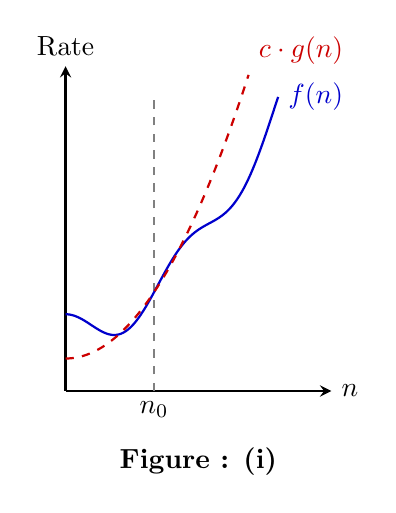
\begin{tikzpicture}[scale=0.75, >=stealth]
  % ===== Figure 1(i): Big-O =====
  % Axes
  \draw[->, thick] (0,0) -- (4.5,0) node[right] {$n$};
  \draw[->, thick] (0,0) -- (0,5.5) node[above] {Rate};
  
  % n0 line
  \draw[dashed, gray, thick] (1.5,0) node[below, text=black] {$n_0$} -- (1.5,5);
  
  % f(n) with slight oscillation that passes exactly through the intersection
  \draw[thick, blue!80!black] 
    plot[domain=0:3.6, samples=100, smooth] 
    (\x, {0.3*\x*\x + 1 + 0.3*sin(180 * (\x - 1.5))}) node[right] {$f(n)$};
    
  % cg(n) Upper bound
  \draw[thick, dashed, red!80!black] 
    plot[domain=0:3.1, samples=80, smooth] 
    (\x, {0.5*\x*\x + 0.55}) node[above right] {$c \cdot g(n)$};

  \node[font=\bfseries] at (2.25,-1.2) {Figure : (i)};
\end{tikzpicture}
\hfill
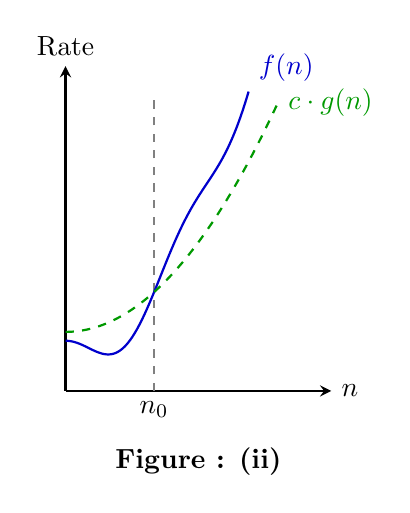
\begin{tikzpicture}[scale=0.75, >=stealth]
  % ===== Figure 1(ii): Omega =====
  % Axes
  \draw[->, thick] (0,0) -- (4.5,0) node[right] {$n$};
  \draw[->, thick] (0,0) -- (0,5.5) node[above] {Rate};
  
  % n0 line
  \draw[dashed, gray, thick] (1.5,0) node[below, text=black] {$n_0$} -- (1.5,5);
  
  % f(n) Upper curve with slight oscillation
  \draw[thick, blue!80!black] 
    plot[domain=0:3.1, samples=100, smooth] 
    (\x, {0.5*\x*\x + 0.55 + 0.3*sin(180 * (\x - 1.5))}) node[above right] {$f(n)$};
    
  % cg(n) Lower bound
  \draw[thick, dashed, green!60!black] 
    plot[domain=0:3.6, samples=80, smooth] 
    (\x, {0.3*\x*\x + 1}) node[right] {$c \cdot g(n)$};

  \node[font=\bfseries] at (2.25,-1.2) {Figure : (ii)};
\end{tikzpicture}
\hfill
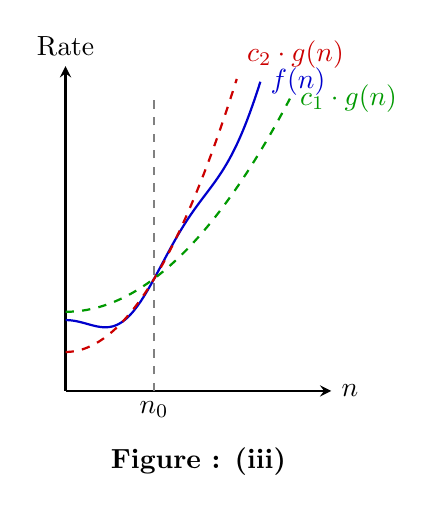
\begin{tikzpicture}[scale=0.75, >=stealth]
  % ===== Figure 1(iii): Theta =====
  % Axes
  \draw[->, thick] (0,0) -- (4.5,0) node[right] {$n$};
  \draw[->, thick] (0,0) -- (0,5.5) node[above] {Rate};
  
  % n0 line
  \draw[dashed, gray, thick] (1.5,0) node[below, text=black] {$n_0$} -- (1.5,5);
  
  % f(n) Middle curve with oscillation
  \draw[thick, blue!80!black] 
    plot[domain=0:3.3, samples=100, smooth] 
    (\x, {0.4*\x*\x + 1 + 0.2*sin(180 * (\x - 1.5))}) node[right] {$f(n)$};
    
  % c2g(n) Upper bound
  \draw[thick, dashed, red!80!black] 
    plot[domain=0:2.9, samples=80, smooth] 
    (\x, {0.55*\x*\x + 0.66}) node[above right] {$c_2 \cdot g(n)$};
    
  % c1g(n) Lower bound
  \draw[thick, dashed, green!60!black] 
    plot[domain=0:3.8, samples=80, smooth] 
    (\x, {0.25*\x*\x + 1.34}) node[right] {$c_1 \cdot g(n)$};

  \node[font=\bfseries] at (2.25,-1.2) {Figure : (iii)};
\end{tikzpicture}
\end{center}

\vspace{0.5cm}

\item Find a tight upper bound on the complexity of the following code segments:
\begin{enumerate}
  \item \begin{verbatim}
void function(int n) {
    int count = 0;
    for (int i=n/2; i<=n; i++)
        for (int j=1; j+n/2<=n; j++)
            for (int k=1; k<=n; k = k*2)
                count++;
}
\end{verbatim}
  \item \begin{verbatim}
void function(int n) {
    int count = 0;
    for (int i=n/2; i<=n; i++)
        for (int j=1; j<=n; j = 2*j)
            for (int k=1; k<=n; k = k*2)
                count++;
}
\end{verbatim}
\end{enumerate}
\mk{10}
\yr{CSE 203 | 2021--22}

\item Deduce the time complexity of the following code fragments:
\begin{enumerate}
  \item \begin{verbatim}
k = 1;
while (n > 1) {
    n = n/2;
    k++;
}
\end{verbatim}
  \item \begin{verbatim}
sum = 0;
for (k=1; k<=n; k*=2)
    for (j=1; j<=k; j++)
        sum++;
\end{verbatim}
\end{enumerate}
\mk{2$\times$6=12}
\yr{CSE 203 | 2020--21}

\item Identify whether the following statements are true or false, clearly justifying your answer:
\begin{enumerate}
  \item If an algorithm has time complexity $O(n^2)$, then it always makes $n^2$ steps.
  \item An algorithm with time complexity $O(n)$ is always slower than an algorithm with time complexity $O(\log n)$, for any input.
  \item An algorithm that makes $c_1 \log_2 n$ steps and an algorithm that makes $c_2 \log_{10} n$ steps are in the same complexity class ($c_1, c_2$ are constants).
  \item An $O(2^n)$ algorithm can never be faster than an $O(n)$ algorithm.
\end{enumerate}
\mk{12}
\yr{CSE 203 | 2020--21}

\item What does the term \textit{asymptotic} mean in complexity analysis? Can we show the worst-case and average-case time complexity using Big-$\Theta$ notation? If yes, how and when? \mk{5+5+5}
\yr{CSE 203 | 2019--20}

\item Derive the time complexity of the following code snippet and write down the asymptotic complexity using Big-$O$ notation. Can we show the complexity using Big-$\Theta$ notation as well? What is the difference in meaning?
\begin{verbatim}
int i, j, k = 0;
for (i = n/2; i <= n; i++) {
    for (j = 2; j <= n; j = j*2) {
        k = k + n/2;
    }
}
\end{verbatim}
\mk{10}
\yr{CSE 203 | 2019--20}

\item Express the following function in $\Theta$ notation with proper explanation:
\[ f(n) = 5n - 2n^2 \]
\mk{8}
\yr{CSE 203 | 2019--20}

\item Suppose that you observe that a program takes 30 seconds to complete on inputs of size 600, 4.5 minutes on inputs of size 1800, and 20 minutes on inputs of size 2000. Develop a reasonable assumption for the order of growth of the running time. \mk{10}
\yr{CSE 203 | 2018--19}

\item What is the difference between Big-$O$ ($O$) and Little-$o$ ($o$) asymptotic notations? Find appropriate $f(n)$ and $g(n)$ (if any) for each of the following cases:
\begin{enumerate}
  \item $f(n) = O(g(n))$, but $g(n) \neq O(f(n))$
  \item $f(n) = O(g(n))$, and $f(n) = \Omega(g(n))$
  \item $f(n) = \Omega(g(n))$, and $f(n) = \omega(g(n))$
  \item $f(n) = \Theta(g(n))$, and $f(n) = o(g(n))$
\end{enumerate}
\mk{5+10}
\yr{CSE 203 | 2017--18}

\item Define Big-$O$, $\Omega$, and $\Theta$ notations. Arrange the following functions in ascending order of growth rate (i.e., if $f(n)$ precedes $g(n)$, then $f(n) = O(g(n))$). Provide justifications.
\[ f_1 = n, \quad f_2 = \log_2 n, \quad f_3 = 2^{\sqrt{\log_2 n}}, \quad f_4 = n \ln n, \quad f_5 = 2^n \]
\mk{6+9}
\yr{CSE 203 | 2016--17}

\item Prove that $15n^4 + 13n^2 + 11n = O(n^4)$, but $15n^4 + 13n^2 + 11n \neq O(n^2)$. \mk{10}
\yr{CSE 203 | 2015--16}

\item  For each of the following pairs indicate whether $f(n)$ is $O(g(n))$, $\Omega(g(n))$ or both \\
(i.e. $\Theta(g(n))$). Provide brief justifications
\begin{center}
\begin{tabular}{|c|c|}
\hline
$f(n)$ & $g(n)$ \\
\hline
$\sqrt{n}$ & $\log_2 n$ \\
\hline
$n^{1.01}$ & $n \log_2^2 n$ \\
\hline
$2^n$ & $2^{n+1}$ \\
\hline
$n!$ & $2^n$ \\
\hline
$n^{100}$ & $1.01^n$ \\
\hline
$\sum_{i=1}^{n} i^k$ & $n^{k+1}$ \\
\hline
\end{tabular}
\end{center}
\mk{6+9=15}
\yr{CSE 207 | 2015--16}

\item What is asymptotic analysis of algorithms? Define Big-$O$, $\Omega$, and $\Theta$ notations. For the functions $f(n) = n\log n$ and $g(n) = 10n\log_{10} n$, show whether $f$ is $O(g)$, or $f$ is $\Omega(g)$, or $f$ is $\Theta(g)$. \mk{3+6+8}
\yr{CSE 207 | 2014--15}

\item Prove that $5n^3 + 3n = O(n^4)$, but $5n^3 + 3n \neq O(n^2)$. \mk{5+5=10}
\yr{CSE 203 | 2012--13}

\item Prove that $O(n^3) \cdot O(n) = O(n^4)$. \mk{5}
\yr{CSE 203 | 2011--12}

\item Write the main three reasons why we usually concentrate on finding the worst-case running time of an algorithm. \mk{5}
\yr{CSE 203 | 2011--12}

\item Why is $n/2 \neq o(n)$? \mk{5}
\yr{CSE 207 | 2009--10}

\item Write down an algorithm for searching $z$ sequentially in array $A$ with $n$ elements. Discuss its average-case, worst-case, and best-case complexities. How can this algorithm be improved? \mk{5+10+5=20}
\yr{CSE 207 | 2008--09}

\item  Define big O-notation, $\Omega$-notation and $\Theta$-notation.

\end{enumerate}
\newpage

\secdivider{Correctness Proof \& Algorithm Analysis}{Master Theorem, Recurrence, Substitution, Loop Invariant}{cC}{cC}
\markboth{T3 --- Correctness Proof \& Algorithm Analysis}{}
\label{sec:T3}
\section{T3 --- Correctness Proof \& Algorithm Analysis}

\begin{enumerate}
\item Analyze the following recurrences using the Master Theorem:
\begin{enumerate}
  \item $T(n) = 2T(n/2) + n\log n$
  \item $T(n) = 2T(n/2) + n^2$
\end{enumerate}
\mk{5+5=10}
\yr{CSE 105 | 2023--24}

\item Using the Master Theorem, prove that Strassen's algorithm improves the runtime of multiplying two $n \times n$ matrices compared to the naive approach with time complexity $O(n^3)$. \mk{10}
\yr{CSE 105 | 2023--24}

\item State the correctness theorem of Breadth-First Search (BFS). Use this theorem to judge whether the value $u.d$ assigned to a vertex $u$ in BFS depends on the order of appearance of the vertices in the corresponding adjacency list. Demonstrate with an example graph whether the breadth-first tree produced by BFS depends on the ordering of vertices in the adjacency lists if the same source vertex is used in every ordering. \mk{17}
\yr{CSE 105 | 2022--23}

\begin{center}
  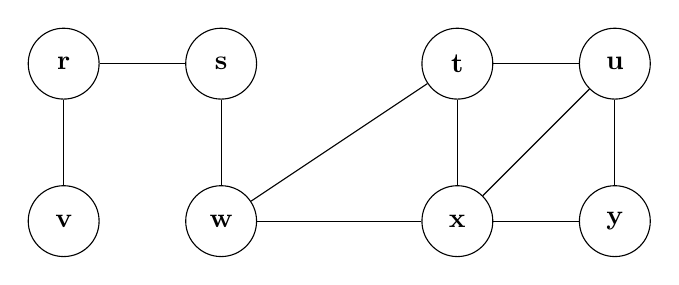
\begin{tikzpicture}[
    every node/.style={circle, draw, minimum size=0.9cm, font=\bfseries},
  ]

  \node (r) at (0, 0)   {r};
  \node (v) at (0, -2)  {v};
  \node (s) at (2, 0)   {s};
  \node (w) at (2, -2)  {w};
  \node (t) at (5, 0)   {t};
  \node (x) at (5, -2)  {x};
  \node (u) at (7, 0)   {u};
  \node (y) at (7, -2)  {y};

  \draw (t) -- (x);
  \draw (r) -- (v);
  \draw (r) -- (s);
  \draw (s) -- (w);
  \draw (w) -- (t);  % cross
  \draw (w) -- (x);
  \draw (t) -- (u);
  \draw (x) -- (u);  % cross
  \draw (x) -- (y);
  \draw (u) -- (y);

  \end{tikzpicture}

\end{center}

\item ``It is asymptotically faster to square an $n$-bit integer than to multiply two $n$-bit integers.'' Do you agree with this statement? Justify your answer. \mk{10}
\yr{CSE 203 | 2021--22}

\item Using the substitution method, solve the following recurrence:
\[ T(n) = 4T\!\left(\frac{n}{2}\right) + 100n^2 \]
\mk{11}
\yr{CSE 203 | 2020--21}

\item Explain whether we can apply the Master Method to any recurrence of the form $T(n) = aT(n/b) + f(n)$. If not, explain a case where the theorem cannot be applied. \mk{8}
\yr{CSE 203 | 2019--20}

\item Traditional insertion sort uses a linear search to scan (backward) through the sorted subarray $A[1\ldots j-1]$, where $A[j]$ is the element to be inserted. Prove or disprove the claim that we can use binary search instead to improve the overall worst-case running time of insertion sort to $\Theta(n \log n)$. \mk{8}
\yr{CSE 203 | 2019--20}

\item Prove or disprove the following: if we choose the element at the middle index as pivot during partition in Quicksort, the algorithm will never have a runtime of $\Theta(n^2)$. \mk{10+8}
\yr{CSE 203 | 2019--20}

\item Consider a divide-and-conquer algorithm: if the problem size is $\leq 5$, it solves the problem in constant time; otherwise, it divides the problem of size $n$ into 4 subproblems each of size $n/3$, solves them recursively, and merges in $O(n)$ time. The division itself takes $O(\sqrt{n} \log n)$ time. Write the recurrence relation for $T(n)$ and solve the following recurrences using the Master Theorem:
\begin{enumerate}
  \item $T(n) = 9T(n/3) + 5n + n^2 + 8\log n$
  \item $T(n) = 3T(n/4) + 3n^2 + 4n + 5$
  \item $T(n) = 4T(n/2) + 5n^3 + 7n$
\end{enumerate}
\mk{10}
\yr{CSE 203 | 2018--19}

\item Suppose you are choosing among three algorithms for multiplying two $n \times n$ matrices:
\begin{enumerate}
  \item Algorithm A (Strassen's) divides each $n \times n$ matrix into four $n/2 \times n/2$ matrices, makes seven recursive calls, and combines them in $\Theta(n^2)$ time.
  \item Algorithm B divides each matrix into twelve $n/3 \times n/3$ matrices, makes nine recursive calls, and combines them in $\Theta(n^2)$ time.
  \item Algorithm C first multiplies two $(n-1) \times (n-1)$ matrices, then combines the result with two vectors of size $n$ in $\Theta(n^2)$ time.
\end{enumerate}
Determine the asymptotic running time of each algorithm (use the Master Theorem where applicable) and determine which algorithm you would choose. \mk{15}
\yr{CSE 203 | 2016--17}

\item Suppose you are choosing among three algorithms for multiplying two $n \times n$ matrices:
\begin{enumerate}
  \item Algorithm A divides each $n \times n$ matrix into four $n/2 \times n/2$ matrices, makes 8 recursive calls, and combines in $\Theta(n^2)$ time.
  \item Algorithm B (Strassen's) divides each $n \times n$ matrix into four $n/2 \times n/2$ matrices, makes 7 recursive calls, and combines in $\Theta(n^2)$ time.
  \item Algorithm C divides each $n \times n$ matrix into nine $n/3 \times n/3$ matrices, makes 9 recursive calls, and combines in $\Theta(n^2)$ time.
\end{enumerate}
Use the Master Theorem to determine asymptotic running times of all three algorithms and choose the best one. \mk{15}
\yr{CSE 207 | 2015--16}

\item State the Master Theorem. Explain why the Master Method cannot be used to solve the recurrence $T(n) = 2T(n/2) + n\log n$. Using the substitution method, prove that $T(n)$ is $O(n\log^2 n)$. \mk{6+6+6}
\yr{CSE 207 | 2014--15}

\item Using the Master Method, prove that the recurrence $T(n) = 3T(n/4) + n\lg n$ solves to $T(n) = \Theta(n\lg n)$. \mk{12}
\yr{CSE 207 | 2009--10}

\item Write the pseudocode of Strassen's algorithm for multiplying two $n \times n$ matrices. Derive the running time. \mk{8+10=18}
\yr{CSE 207 | 2009--10}

\end{enumerate}
\newpage

\secdivider{Arrays, Linked Lists, Stacks \& Queues}{Linear Data Structures, Implementation, Operations}{cD}{cD}
\markboth{T4 --- Arrays, Linked Lists, Stacks \& Queues}{}
\label{sec:T4}
\section{T4 --- Arrays, Linked Lists, Stacks \& Queues}

\begin{enumerate}
\item You are asked to merge two singly linked lists whose elements are sorted in ascending order. The output list will also be sorted in ascending order. Sketch an algorithm to solve the problem. Analyze that your algorithm runs in linear time on the number of elements of the output list. \mk{15}
\yr{CSE 105 | 2023--24}

%% ---------------------------------------------------------------------
%% Q1. Merge two sorted singly linked lists
%% ---------------------------------------------------------------------

\item You are given two linked lists of unsorted elements. Investigate whether you can develop a constant time algorithm to concatenate them if both of the lists are (i) singly linked lists (SLL), (ii) doubly linked list (DLL), (iii) circular SLL, (iv) circular DLL. If yes, sketch the algorithm and examine its correctness; otherwise demonstrate why a constant time algorithm is not possible. \mk{20}
\yr{CSE 105 | 2023--24}

\item Assume that a string contains only left and right parentheses which may or may not be balanced and properly nested. For example, the string \texttt{``((()())()''} contains properly nested pairs of parentheses, but the string \texttt{``)()(''} does not, and the string \texttt{``())''} does not contain properly matching parentheses. Using a stack, construct an algorithm that returns \texttt{true} if a string contains properly nested and balanced parentheses, and \texttt{false} otherwise. Modify the algorithm so that it returns the position in the string of the first offending parenthesis if the string is not properly nested and balanced --- if an excess right parenthesis is found, return its position; if there are too many left parentheses, return the position of the first excess left parenthesis. Return $-1$ if the string is properly balanced and nested. Assume indices start from 0. \mk{25}
\yr{CSE 105 | 2023--24}

%% ---------------------------------------------------------------------
%% Q3. Parenthesis balancing using a stack
%% ---------------------------------------------------------------------

%% ---------------------------------------------------------------------
\item Given an integer $k$ and a queue of integers, how do you reverse the order of the first $k$ elements of the queue, leaving the other elements in the same relative order? For example, if $k = 4$ and the queue has the elements $[10, 20, 30, 40, 50, 60, 70, 80, 90]$, the output should be $[40, 30, 20, 10, 50, 60, 70, 80, 90]$. \mk{10}
\yr{CSE 105 | 2023--24}

%%---------------------------------------------------------------------
%% Q2: Circular Queue using array
%%---------------------------------------------------------------------
\item Implement a Circular Queue using an array. Include: \texttt{enqueue(x)},
\texttt{dequeue()}, \texttt{is\_empty()}, \texttt{is\_full()}, \texttt{front()}.
\mk{15}
\yr{CSE 105 | 2022--23}

%%---------------------------------------------------------------------
%% Q3: Delete node from doubly linked list
%%---------------------------------------------------------------------
\item Write a function to delete a node with a given key from a doubly linked
list (unique keys, access to both \texttt{head} and \texttt{tail}). \mk{10}
\yr{CSE 105 | 2022--23}

%%---------------------------------------------------------------------
%% Q4: Reverse a singly linked list (pseudocode)
%%---------------------------------------------------------------------
\item How would you reverse a singly linked list (without duplicating the list)?
Write the steps (pseudocode) conceptually. \mk{4}
\yr{CSE 105 | 2022--23}

%%---------------------------------------------------------------------
%% Q5: Remove duplicates from sorted singly linked list
%%---------------------------------------------------------------------
\item How can you remove duplicate values from a sorted singly linked list?
\mk{5}
\yr{CSE 105 | 2022--23}

%%---------------------------------------------------------------------
%% Q6: Check if singly linked list is a palindrome
%%---------------------------------------------------------------------
\item How can you check if a singly linked list is a palindrome? Write the steps
involved conceptually. \mk{10}
\yr{CSE 105 | 2022--23}

%%---------------------------------------------------------------------
%% Q7: Advantages/Disadvantages of Arrays vs Linked Lists
%%---------------------------------------------------------------------
\item Given an array of integers (with both negative and positive numbers), write a program to find the $K$-th largest sum of a contiguous subarray within the array. \mk{10}
\yr{CSE 203 | 2021--22}

\item Suppose the numbers $0, 1, 2, \ldots, 9$ were pushed onto a stack in that order, but pops occurred at random points between the various pushes. Determine which of the following two sequences is a valid pop sequence and explain why:
\[S_1: 3,2,6,5,7,4,1,0,9,8\]
\[S_2: 3,2,6,4,7,5,1,0,9,8\]
\mk{3}
\yr{CSE 105 | 2021--22}

\item  A stack is being used to parse matching parentheses, brackets, and braces --- \texttt{(}, \texttt{[}, and \texttt{\{}. Show the state of the stack at the end of the given code fragment. \mk{10}
\yr{CSE 105 | 2021--22}

\begin{lstlisting}[style=cppstyle]
#include <iostream>
using namespace std;

int main()
{
    const int M = 30;
    int N = 1024;
    int parent[N], height[N], depth[N];
    int maxheights[100];
    for (int i = 0; 1 < 100; ++i)
    {
        maxheights[i] = 0;
    }
    double minmeandepth = 1e300;
    double meandepths = 0;
    double maxmeandepth = 0;
    for (int j = 0; j < M; ++j)
    {
    for (int i = 0; i < N; ++i)
    {
        parent[i] = -1;
        height[i] = 0;
    }
    for (int i = 0; i < N - 1; ++i)
    while (true)
    {
    int pl = rand() & (N - 1);
    int p2 = rand() & (N - 1);

    int s1 = pi1;
    int s2 = p2;

    while ( parent[
\end{lstlisting}

\item You are given access to the following functions of a list data structure:
\begin{itemize}
  \item \texttt{init(n)} --- Initialize an array $L[0..n-1]$ of length $n$ for integers. Current position `points to' $L[0]$. All the functions below are applied on this array which is not accessible directly.
  \item \texttt{insert(item)} --- Inserts an element at the current position and current position is `incremented' (so if current position pointed to $L[k]$ before the call, after the call it points to $L[k+1]$). Here, \textit{item} is the element to be inserted. In case the list is full, it returns ERR (a large negative constant).
  \item \texttt{remove()} --- Removes the element at the current position and current position is `decremented' (so if current position pointed to $L[k]$ before the call, after the call it points to $L[k-1]$). In case the list is empty, it returns ERR (a large negative constant).
  \item \texttt{value()} --- Returns the value of the element at the current position. Current position remains unchanged. In case the list is empty, it returns ERR (a large negative constant).
  \item \texttt{moveToStart()} --- Sets the current position to $L[0]$.
  \item \texttt{moveToEnd()} --- Sets the current position to $L[n-1]$.
  \item \texttt{next()} --- Increments the current position (so if current position pointed to $L[k]$ before the call, after the call it points to $L[k+1]$). If $k = n-1$, it returns ERR (a large negative constant).
  \item \texttt{prev()} --- Decrements the current position (so if current position pointed to $L[k]$ before the call, after the call it points to $L[k-1]$). If $k = 0$, it returns ERR (a large negative constant).
\end{itemize}
Now you have to build one queue and one stack in one List data structure as defined above. The queue should grow from the beginning of the list (i.e., first element of the queue should be at $L[0]$) and the stack should grow from the end of the list (i.e., the first element of the stack should be at $L[n-1]$). You have no access to the code of the above implementation and can only call these functions in your code. You need to write appropriate codes (no specific programming language is required; pseudo code is fine) for implementing the queue and stack simultaneously as described above. Please explain your code by giving appropriate comments. In particular, you need to implement the following four functions:
\begin{itemize}
  \item \texttt{push(item)} --- push a positive integer, \textit{item} in the stack. If there is an error (e.g., no more space available for growing the stack in the list), it should output an appropriate error message and return with $-1$.
  \item \texttt{pop()} --- pop an element from the stack. If there is an error, it should output an appropriate error message and return with $-1$.
  \item \texttt{enqueue(item)} --- enqueue a positive integer, \textit{item} in the queue. If there is an error (e.g., no more space available for growing the queue in the list), it should output an appropriate error message and return with $-1$.
  \item \texttt{dequeue()} --- dequeue an element from the queue. If there is an error, it should output an appropriate error message and return with $-1$.
\end{itemize}
\mk{25}
\yr{CSE 105 | 2021--22}

\item Convert a Binary Tree to a Circular Doubly Linked List using inorder
traversal (left/right pointers become prev/next). \mk{15}
\yr{CSE 203 | 2021--22}

%%═══════════════════════════════════════════════════════════════════
%% Q13  KStacks --- two stacks in one array
%%═══════════════════════════════════════════════════════════════════
\item Create \texttt{KStacks}: two stacks in a single array efficiently. Implement push1,pop1,\\push2,pop2. \mk{10}
\yr{CSE 203 | 2021--22, 2016--17}

%%═══════════════════════════════════════════════════════════════════
%% Q14  Longest valid parentheses substring
%%═══════════════════════════════════════════════════════════════════

\item Given a string consisting of opening and closing parentheses, find the length of the longest valid parenthesis substring. \mk{10}
\yr{CSE 203 | 2021--22}

%%═══════════════════════════════════════════════════════════════════
%% Q15  Stack using Queue(s)
%%═══════════════════════════════════════════════════════════════════
\item Given a Queue data structure that supports \texttt{enqueue()} and \texttt{dequeue()}, implement a Stack using only instances of Queue and Queue operations. \mk{10}
\yr{CSE 203 | 2021--22}

%%═══════════════════════════════════════════════════════════════════
%% Q16  Flatten multilevel linked list (BFS / level-by-level)
%%═══════════════════════════════════════════════════════════════════

\item Given a linked list where in addition to the next pointer, each node has a
child pointer, which may or may not point to a separate list. These child lists
may have one or more children of their own, and so on, to produce a multilevel
data structure, as shown in Figure . You are given the head of the
first level of the list. Flatten the list so that all the nodes appear in a
single-level linked list. You need to flatten the list in a way that all nodes
at the first level should come first, then nodes of second level, and so on.

\begin{center}
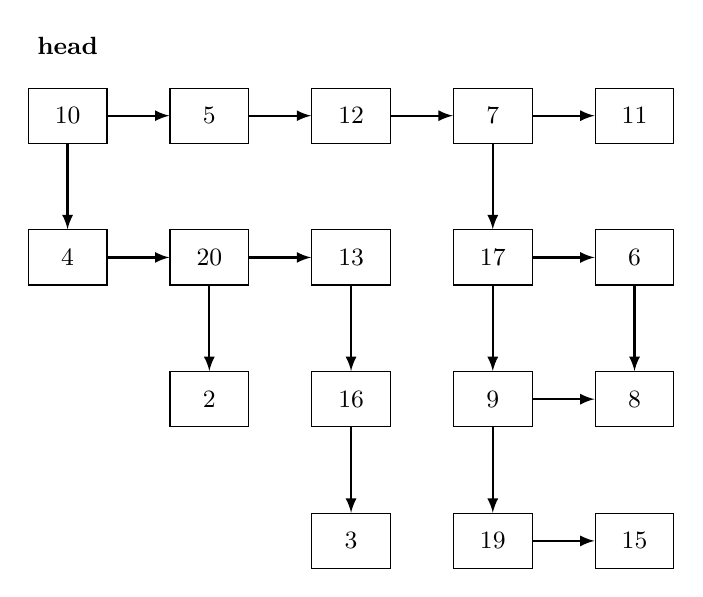
\begin{tikzpicture}[
  box/.style={draw, minimum width=10mm, minimum height=7mm, font=\small},
  arr/.style={->, >=latex, thick},
  carr/.style={->, >=latex, thick},
  node distance=0mm
]
%% Level 1
\node[box] (n10) at (0,    0)  {10};
\node[box] (n5)  at (1.8,  0)  {5};
\node[box] (n12) at (3.6,  0)  {12};
\node[box] (n7)  at (5.4,  0)  {7};
\node[box] (n11) at (7.2,  0)  {11};
\node[font=\small, above=3mm of n10] {\textbf{head}};

\draw[arr] (n10)--(n5);
\draw[arr] (n5)--(n12);
\draw[arr] (n12)--(n7);
\draw[arr] (n7)--(n11);

%% Level 2 left: 4$\rightarrow$20$\rightarrow$13
\node[box] (n4)  at (0,   -1.8) {4};
\node[box] (n20) at (1.8, -1.8) {20};
\node[box] (n13) at (3.6, -1.8) {13};

\draw[arr] (n4)--(n20);
\draw[arr] (n20)--(n13);

%% Level 2 right: 17$\rightarrow$6
\node[box] (n17) at (5.4, -1.8) {17};
\node[box] (n6)  at (7.2, -1.8) {6};

\draw[arr] (n17)--(n6);

%% Child arrows level1 $\rightarrow$ level2
\draw[carr] (n10.south)--(n4.north);
\draw[carr] (n7.south)--(n17.north);

%% Level 3: 2, 16, 9$\rightarrow$8
\node[box] (n2)  at (1.8, -3.6) {2};
\node[box] (n16) at (3.6, -3.6) {16};
\node[box] (n9)  at (5.4, -3.6) {9};
\node[box] (n8)  at (7.2, -3.6) {8};

\draw[arr] (n9)--(n8);

%% Child arrows level2 $\rightarrow$ level3
\draw[carr] (n20.south)--(n2.north);
\draw[carr] (n13.south)--(n16.north);
\draw[carr] (n17.south)--(n9.north);
\draw[carr] (n6.south)--(n8.north);

%% Level 4: 3, 19$\rightarrow$15
\node[box] (n3)  at (3.6, -5.4) {3};
\node[box] (n19) at (5.4, -5.4) {19};
\node[box] (n15) at (7.2, -5.4) {15};

\draw[arr] (n19)--(n15);

%% Child arrows level3 $\rightarrow$ level4
\draw[carr] (n16.south)--(n3.north);
\draw[carr] (n9.south)--(n19.north);

\end{tikzpicture}

\smallskip
\end{center}

The above list should be converted to
$10 \to 5 \to 12 \to 7 \to 11 \to 4 \to 20 \to 13 \to 17
\to 6 \to 2 \to 16 \to 9 \to 8 \to 3 \to 19 \to 15$. \mk{15}\yr{CSE 203 | 2021--22}

%%═══════════════════════════════════════════════════════════════════
%% Q17  Reverse a stack using recursion (no loops)
%%═══════════════════════════════════════════════════════════════════
\item Write a program to reverse a stack using recursion, without using any loop. \mk{10}
\yr{CSE 203 | 2021--22}

\item Why is Binary Search preferred over Ternary Search? \mk{10}
\yr{CSE 203 | 2021--22}

\item Write a code snippet to implement a queue using a circular array, where
each element contains ID, name, and department of a student. \mk{13}
\yr{CSE 203 | 2019--20}

%%═══════════════════════════════════════════════════════════════════
%% Q8  File system DFS hierarchy print
%%═══════════════════════════════════════════════════════════════════
\item Consider the following hierarchical structure of a file system. Write a
program to print the directory hierarchy of the file system, where all children
of a parent will be placed one tab-space right from the parent. Use depth-first
tree traversal technique to perform the above task.

\begin{center}
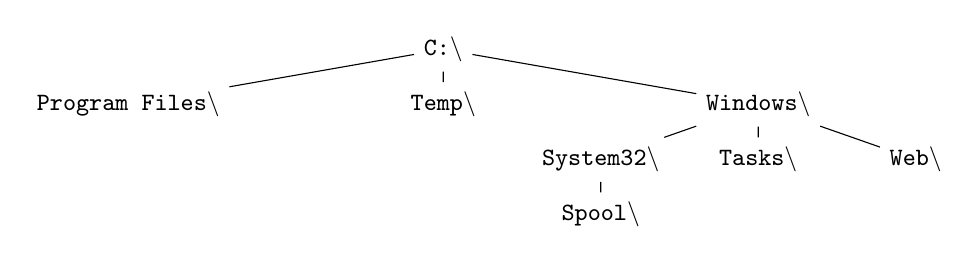
\begin{tikzpicture}[
  every node/.style={font=\small},
  edge from parent/.style={draw},
  level distance=7mm,
  level 1/.style={sibling distance=40mm},
  level 2/.style={sibling distance=20mm},
  level 3/.style={sibling distance=18mm}
]
\node {\texttt{C:\textbackslash}}
  child { node {\texttt{Program Files\textbackslash}} }
  child { node {\texttt{Temp\textbackslash}} }
  child { node {\texttt{Windows\textbackslash}}
    child { node {\texttt{System32\textbackslash}}
      child { node {\texttt{Spool\textbackslash}} }
    }
    child { node {\texttt{Tasks\textbackslash}} }
    child { node {\texttt{Web\textbackslash}} }
  };
\end{tikzpicture}
\end{center}
\mk{12}\yr{CSE 203 | 2019--20}

%%═══════════════════════════════════════════════════════════════════
%% Q9  Stack using List ADT (with max())
%%═══════════════════════════════════════════════════════════════════
\item Give the algorithm for converting an infix expression to postfix, and
for evaluating a postfix expression using a stack. \mk{10}
\yr{CSE 203 | 2018--19}

%%═══════════════════════════════════════════════════════════════════
%% Q5  Ternary Search
%%═══════════════════════════════════════════════════════════════════
\item Ternary search, like binary search, is a divide-and-conquer algorithm. It is
mandatory for the array (in which you will search for an element) to be sorted
before you begin the search. In this search, after each iteration it neglects
$\frac{2}{3}$ part of the array and repeats the same operations on the remaining
$\frac{1}{3}$. Write an algorithm for ternary search and show its complexity.
\mk{12}\yr{CSE 203 | 2018--19}

%%═══════════════════════════════════════════════════════════════════
%% Q6  Array better than linked list --- scenario
%%═══════════════════════════════════════════════════════════════════
\item Describe a situation where storing items in an array is clearly better
than storing items in a linked list. \mk{8}
\yr{CSE 203 | 2018--19}

%%═══════════════════════════════════════════════════════════════════
%% Q7  Circular Queue with struct (Student: ID, name, dept)
%%═══════════════════════════════════════════════════════════════════
\item Write two versions of binary search. Simulate on $[23,56,8,10,12,15,
20,21,23]$ for keys $1, 6, 23, 24$. \mk{10+10=20}
\yr{CSE 203 | 2017--18}

%%═══════════════════════════════════════════════════════════════════
%% Q4  Infix -> Postfix + evaluate postfix
%%═══════════════════════════════════════════════════════════════════
\item How do we cope with hard problems? Discuss. \mk{10}
\yr{CSE 207 | 2017--18}

\item Given a singly linked list and integers $m$ and $k$, find the node with
value $m$ then delete the next $k$ nodes. \mk{10}
\yr{CSE 203 | 2016--17}

%%---------------------------------------------------------------------
%% Q22: Two stacks in a single array
%%---------------------------------------------------------------------

\item Write \texttt{enqueue} and \texttt{dequeue} functions for a FIFO queue
implemented using a singly linked list. \mk{10}
\yr{CSE 203 | 2016--17}

%%═══════════════════════════════════════════════════════════════════
%% Q3  Binary Search (two versions + simulation)
%%═══════════════════════════════════════════════════════════════════
\item Deduce the condition under which an array-based implementation of a list
would be better in space utilisation than a linked-based implementation. \mk{10}
\yr{CSE 203 | 2015--16}

%%---------------------------------------------------------------------
%% Q17: w#w' check using a stack
%%---------------------------------------------------------------------
\item Given input string $x$, check whether $x$ is of the form $w\#w'$, where
$w'$ is the reverse of $w$. Suggest a data structure and show how to solve it
efficiently. \mk{10}
\yr{CSE 203 | 2015--16}

%%---------------------------------------------------------------------
%% Q18: n-th node before the one containing key k
%%---------------------------------------------------------------------
\item Given input $k$ and $n$, return the key of the $n$-th node before the
one containing $k$. (All keys distinct.) \mk{15}
\yr{CSE 203 | 2015--16}

%%---------------------------------------------------------------------
%% Q19: Array-based stack: beginning as top --- efficient?
%%---------------------------------------------------------------------
\item Your group proposes that the beginning (index 0) of the array be the top
of the stack. A friend claims this is inefficient. Do you agree? Justify. \mk{8}
\yr{CSE 203 | 2015--16}

%%---------------------------------------------------------------------
%% Q20: Drifting Queue Problem
%%---------------------------------------------------------------------
\item Discuss the Drifting Queue Problem with an illustrative example. Propose
a solution. Address empty/full recognition. \mk{5+5+5+4=19}
\yr{CSE 203 | 2015--16}

%%---------------------------------------------------------------------
%% Q21: Delete next k nodes after node with value m
%%---------------------------------------------------------------------
\item What is an application of prefix sums? What are prefix sums of an array
$A[i]$, $1 \leq i \leq n$? Write a parallel algorithm that finds prefix sums of
the array $A$. Illustrate for $[15,35,40,25,20,50,10,30]$ showing bottom-up and
top-down traversals. \mk{15}
\yr{CSE 207 | 2015--16}

%%---------------------------------------------------------------------
\item Implement \texttt{void delete(int N)} that deletes all $M$th nodes such
that $M \bmod N = 0$ from the doubly linked list (head is the 1st node). \mk{15}
\yr{CSE 203 | 2014--15}

%%---------------------------------------------------------------------
%% Q11: ArrayList vs LinkedList complexity comparison
%%---------------------------------------------------------------------
\item Compare worst-case run times of ArrayList and LinkedList (doubly, with
head and tail) for the listed operations. \mk{4$\times$3=12}
\yr{CSE 203 | 2014--15}

%%---------------------------------------------------------------------
%% Q12: Two advantages/disadvantages of array-based lists over linked lists
%%---------------------------------------------------------------------
\item Give two advantages and disadvantages of using array-based lists over
linked lists. \mk{8}
\yr{CSE 203 | 2014--15}

%%---------------------------------------------------------------------
%% Q13: Stack using singly linked list (push, pop, size)
%%---------------------------------------------------------------------
\item Implement a \textbf{stack} using a singly linked list (\texttt{push},
\texttt{pop}, \texttt{size}). Only \texttt{head} and \texttt{tail} pointers;
no other global/static variables. \mk{15}
\yr{CSE 203 | 2014--15}

%%---------------------------------------------------------------------
%% Q14: Amortised O(1) per insertion with doubling
%%---------------------------------------------------------------------
\item Suppose we double the memory of an array-based list every time it is full
during insertion. Show the average time per insertion for copying is constant.
\mk{12}
\yr{CSE 203 | 2014--15}

%%---------------------------------------------------------------------
%% Q15: Reasons to use restrictive data structures
%%---------------------------------------------------------------------
\item Give two reasons why we should use restrictive data structures (e.g.,
Stack, Queue) instead of general-purpose ones (e.g., List). \mk{4}
\yr{CSE 203 | 2014--15}

%%---------------------------------------------------------------------
%% Q16: Array vs linked list space utilisation
%%---------------------------------------------------------------------
\item Given a doubly linked list and an integer $n$, write a function \texttt{deleteLastNElements()} that deletes the last $n$ nodes from the given linked list. \mk{8}
\yr{CSE 203 | 2013--14}

\item How do you implement a Queue using a Stack? What are the running times of \texttt{enqueue} and \texttt{dequeue} operations of such an implementation? \mk{8+2=10}
\yr{CSE 203 | 2013--14}

\item Which type of traversal will traverse the binary tree \texttt{BUETCSE12} (as shown in figure)? Write an algorithm for such traversal of a binary tree using a Stack or Queue. \mk{2+10=12}
\yr{CSE 203 | 2013--14}

\begin{center}
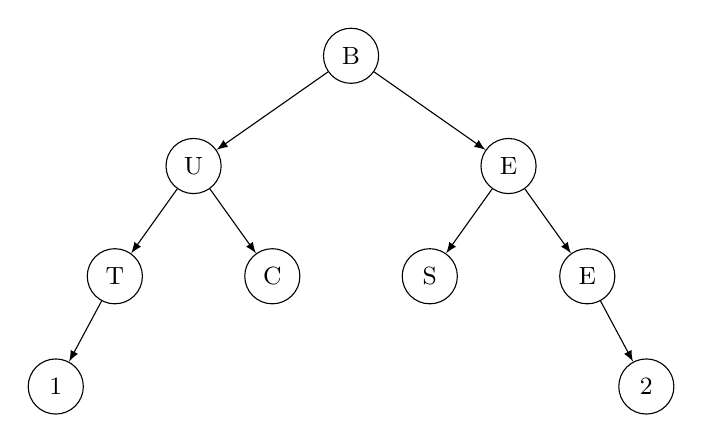
\begin{tikzpicture}[
  every node/.style={circle, draw, minimum size=7mm, font=\small},
  level distance=14mm,
  level 1/.style={sibling distance=40mm},
  level 2/.style={sibling distance=20mm},
  level 3/.style={sibling distance=15mm},
  edge from parent/.style={draw, -latex}
]
\node {B}
  child { node {U}
    child { node {T}
      child { node {1} }
      child[missing] {}
    }
    child { node {C} }
  }
  child { node {E}
    child { node {S} }
    child { node {E}
      child[missing] {}
      child { node {2} }
    }
  };
\end{tikzpicture}
\end{center}

\item Give 2 (two) real-life applications each for: (i) Stack, (ii) Queue, (iii) Priority Queue. \mk{2+2+2=6}
\yr{CSE 203 | 2013--14}

\item Write pseudocodes for \texttt{enqueue} and \texttt{dequeue} operations for the array implementation of a circular queue. \mk{7}
\yr{CSE 203 | 2013--14}

\item Give a comparison of array and linked list. \mk{6}
\yr{CSE 203 | 2013--14}

%%---------------------------------------------------------------------
\item Write down a linear-time algorithm for finding the maximum sum of a
consecutive subsequence of an array. \mk{15}
\yr{CSE 207 | 2013--14}

%%---------------------------------------------------------------------
\item Write two functions for the insertion and deletion operations in a
circular linked list. \mk{5+5=10}
\yr{CSE 203 | 2012--13}

%%---------------------------------------------------------------------
%% Q10: Delete every Nth node from doubly linked list
%%---------------------------------------------------------------------
\item Explain the advantages and disadvantages of arrays and linked lists. \mk{5}
\yr{CSE 203 | 2011--12}

%%---------------------------------------------------------------------
%% Q8: Insert and Delete for Circular Queue (pseudocode)
%%---------------------------------------------------------------------
\item Write pseudocodes for the \texttt{Insert} and \texttt{Delete} operations
of a circular queue. \mk{6}
\yr{CSE 203 | 2011--12}

%%---------------------------------------------------------------------
%% Q9: Insert and Delete for Circular Linked List
%%---------------------------------------------------------------------
\item Write down a linear-time algorithm for computing the maximum sum of a
consecutive subsequence. Simulate the algorithm on the following array, showing
values of \texttt{maxsum} and \texttt{suffixmax}:
\[ 2, -1, 3, 1, 2, -4, 5, 2, -3, 7, 2, 4, -1, 2, -3 \]
\mk{15}
\yr{CSE 207 | 2007--08}

%%---------------------------------------------------------------------

\item Suppose you are given an implementation of a list Abstract Data Type (ADT)
which has the functions listed in Table~A. Implement a stack which has the
functionality shown in Table~B. In your implementation, you can only use the list
implementation of Table~A. Assume that the elements are integers.\mk{15}

%%═══════════════════════════════════════════════════════════════════
%% Q10  Independent max() using only the stack (no list ADT)
%%═══════════════════════════════════════════════════════════════════
\item Your friend uses your above stack implementation regularly. A bug has been
reported for the \texttt{max()} function of your stack implementation. Now your
friend needs to implement a separate independent \texttt{max()} function which uses
the stack data structure (avoiding its own \texttt{max()} function). He does not
have access to the list data structure of Table~A. How will he implement the
\texttt{max()} function? He cannot use any data structure other than your stack
implementation. \mk{10}

%%═══════════════════════════════════════════════════════════════════
%% Q11  addBook into publisher-grouped DLL
%%═══════════════════════════════════════════════════════════════════

\item We use a doubly linked list (DLL) to keep records of some books. In the list,
all the books that belong to the same publisher are placed in consecutive nodes.
Now, write a function \texttt{addBook(title, publisher)} that inserts a book into
the DLL as the first book for its publisher. So, if the list already has three books
for a particular publisher, the 4\textsuperscript{th} book will be inserted in
front of the three books already in the DLL. For a new publisher, the book should
be inserted at the end of the DLL. Assume that each DLL node has `prev' and `next'
pointers and stores the title and publisher of a book as Strings. \mk{10}

%%═══════════════════════════════════════════════════════════════════
%% Q12  Binary Tree -> Circular Doubly Linked List (inorder)
%%═══════════════════════════════════════════════════════════════════
\item Suppose Figure~8.b-I gives a snapshot of the memory at one point. You are
running your program for a linked list based list implementation. In your
implementation each node has two variables: an integer \textit{key} and a pointer
\textit{ptr}. The current situation of the list is illustrated in Figure~8.b-II. You
have further implemented the concept of freelist so as to minimize the number of
calls to `new' and `delete'. The first, second, third and fourth (i.e., last) node
correspond to address 1, 2, 3 and 4 in the memory respectively. Suppose at this
point a delete operation is done for the node containing 29 followed by two append
operations of two nodes containing values 1111 and 2222 respectively.

\begin{center}
\begin{tabular}{@{}|c|c|@{}}
\hline
\textbf{Address} & \textbf{Values at Memory Location} \\
\hline
0  & $-31$ \\
1  & 12 \\
2  & 14 \\
3  & 29 \\
4  & 100 \\
5  & 112 \\
6  & 4 \\
$\ldots$ & $\ldots$ \\
\hline
\end{tabular}
\end{center}

\begin{center}
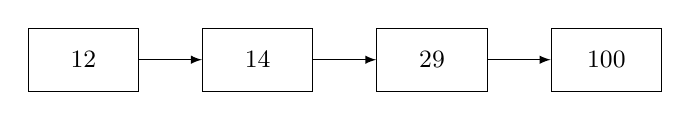
\begin{tikzpicture}[
  node distance=0mm,
  box/.style={draw, minimum width=14mm, minimum height=8mm, font=\small}
]
\node[box] (n1) {12};
\node[box, right=8mm of n1] (n2) {14};
\node[box, right=8mm of n2] (n3) {29};
\node[box, right=8mm of n3] (n4) {100};

\draw[->, >=latex] (n1.east) -- (n2.west);
\draw[->, >=latex] (n2.east) -- (n3.west);
\draw[->, >=latex] (n3.east) -- (n4.west);
\end{tikzpicture}

\smallskip
\textit{Figure 8.b-II}
\end{center}

\begin{enumerate}[label=(\roman*)]
  \item Draw the updated list after each operation.
  \item Provide the value of \textit{ptr} variable for each node in Figure~8.b-II
  before and after the delete operation. If a node remains in the memory after
  your deletion operation, you would need to provide the value of the \textit{ptr}
  variable of that node as well.
  \item Provide the updated values of each memory cell after the two operations
  (delete and append) are complete.
\end{enumerate}

You can assume that the next call of C\texttt{++} `new' operator will return the
address 5. \mk{5+10+10=25}

%%═══════════════════════════════════════════════════════════════════
%% Q2  Enqueue / Dequeue with singly linked list
%%═══════════════════════════════════════════════════════════════════
\end{enumerate}
\newpage

\secdivider{Trees \& Tree Traversals}{Binary Trees, General Trees, Traversal Algorithms}{cE}{cE}
\markboth{T5 --- Trees \& Tree Traversals}{}
\label{sec:T5}
\section{T5 --- Trees \& Tree Traversals}

\begin{enumerate}
\item Analyze the maximum and minimum number of nodes in a binary tree of height $h$. \mk{10}
\yr{CSE 105 | 2023--24}

%% ---------------------------------------------------------------------
%% Q: Analyze the maximum and minimum number of nodes in a binary tree
%%    of height h.  [CSE 105 | 2023--24]
%% ---------------------------------------------------------------------

\item Prove the following theorems that describe the properties of perfect binary trees:
\begin{enumerate}
  \item A perfect tree has $2^{h+1} - 1$ nodes.
  \item The average depth of a node is $\Theta(\ln n)$.
\end{enumerate}
\mk{4+6=10}
\yr{CSE 105 | 2022--23}
%% ---------------------------------------------------------------------
%% Q: Prove properties of perfect binary trees (2 parts).
%%    [CSE 105 | 2022--23]
%% ---------------------------------------------------------------------

\item You are given a tree of size $n$ as an array \texttt{parent[0..n-1]}, where every index $i$ represents a node and \texttt{parent[i]} is its immediate parent ($-1$ for the root). Write an algorithm to find the height of the generic tree.
\begin{center}
\texttt{Input: parent[] = \{-1, 0, 0, 0, 3, 1, 1, 2\} \quad Output: 2}
\end{center}
\mk{15}
\yr{CSE 203 | 2021--22}
%% ---------------------------------------------------------------------
%% Q: Height of generic tree stored as parent[] array.
%%    parent[] = {-1,0,0,0,3,1,1,2}  Output: 2
%%    [CSE 203 | 2021--22]
%% ---------------------------------------------------------------------

\item Write two procedures for finding the successor element and the predecessor element in a binary search tree. Write the preorder, inorder, and postorder traversal sequences of the binary tree whose Euler tour traversal sequence is \texttt{a e h i h e a c b f b g b c d j d c a}. Also draw the binary tree. \mk{10+15}
\yr{CSE 203 | 2016--17}
%% ---------------------------------------------------------------------
%% Q: Successor & Predecessor in BST; Euler-tour to pre/in/post-order.
%%    Euler tour: a e h i h e a c b f b g b c d j d c a
%%    [CSE 203 | 2016--17]
%% ---------------------------------------------------------------------

\item Suppose the tree is an unordered tree (i.e., the order of children is not relevant). Determine whether each of the following breadth-first traversals is valid or not, with justification:
\begin{enumerate}
  \item \texttt{G F B K E C A I N J D H M L O}
  \item \texttt{G F B K E C A I N J D H M L O}
  \item \texttt{G K F B I J N E A C O M L H D}
  \item \texttt{G F B K E C A I N J O M L H D}
\end{enumerate}
\mk{16}
\yr{CSE 203 | 2015--16}
\begin{center}
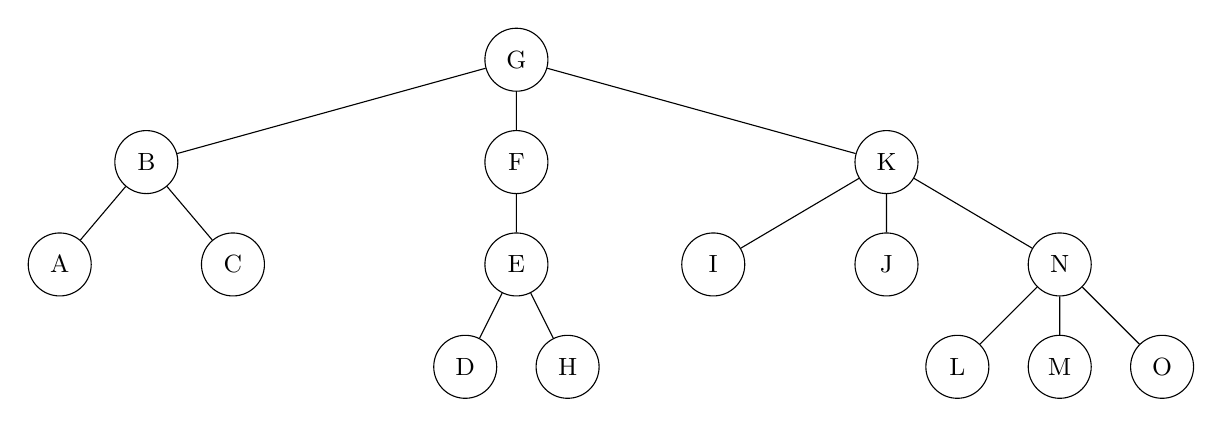
\begin{tikzpicture}[
  every node/.style={circle, draw, minimum size=8mm, font=\small},
  level distance=13mm,
  level 1/.style={sibling distance=47mm},
  level 2/.style={sibling distance=22mm},
  level 3/.style={sibling distance=13mm}
]
\node {G}
  child { node {B}
    child { node {A} }
    child { node {C} }
  }
  child { node {F}
    child { node {E}
      child { node {D} }
      child { node {H} }
    }
  }
  child { node {K}
    child { node {I} }
    child { node {J} }
    child { node {N}
      child { node {L} }
      child { node {M} }
      child { node {O} }
    }
  };
\end{tikzpicture}
\end{center}

\item Suppose that we are given the following definition of a rooted binary tree
(\textbf{not binary search tree}):
\begin{verbatim}
struct treeNode
{
    int item ;               //stores the value
    struct treeNode * left ; //points to left child
    struct treeNode * right ;//points to right child
} ;
struct treeNode * root ; //global variable to store tree root node
\end{verbatim}
Implement the following function \textit{clone} (\textbf{must be recursive}) that
makes a copy of a binary tree (keeping the original tree intact). The function will
be called using the original root pointer as input argument. The function should
return the root node of the new copy. For example calling $x = clone(root)$ will
return the new root (of the tree copy) into variable $x$.
\begin{verbatim}
struct treeNode * clone(struct treeNode * node);
\end{verbatim}
\mk{12}
\yr{CSE 203 | 2014--15}

%% ---------------------------------------------------------------------
%% Q: clone() --- recursive copy of binary tree.  [CSE 203 | 2014--15]
%% ---------------------------------------------------------------------

\item What is a proper binary tree? Construct the proper binary tree whose inorder and postorder traversals are given as:
\begin{itemize}
  \item \textbf{Inorder:} \texttt{BUETCSE12}
  \item \textbf{Postorder:} \texttt{BEUCTES21}
\end{itemize}
\mk{2+8=10}
\yr{CSE 203 | 2013--14}
%% ---------------------------------------------------------------------
%% Q: Proper binary tree from inorder + postorder.
%%    Inorder:   B U E T C S E 1 2
%%    Postorder: B E U C T E S 2 1
%%    [CSE 203 | 2013--14]
%% ---------------------------------------------------------------------

\item Draw a binary tree whose preorder and inorder traversals both yield \texttt{BUETCSE12}. \mk{7}
\yr{CSE 203 | 2013--14}
%% ---------------------------------------------------------------------
%% Q: Draw a binary tree whose preorder and inorder are both
%%    BUETCSE12.   [CSE 203 | 2013--14]
%% ---------------------------------------------------------------------

\item What is a tree? Write a linear-time algorithm for finding the height of a tree. Analyze the time complexity of the algorithm. \mk{1+4+4=9}
\yr{CSE 203 | 2012--13 , 2011--12}
%% ---------------------------------------------------------------------
%% Q: Linear-time height algorithm.  [CSE 203 | 2012--13]
%% ---------------------------------------------------------------------

\item Let $T$ be a proper binary tree with height $h$. Prove that the number of internal nodes in $T$ is at least $h$ and at most $2^h - 1$. \mk{4+4=8}
\yr{CSE 203 | 2012--13 , 2011--12}
%% ---------------------------------------------------------------------
%% Q: Proper binary tree, height h. Prove internal nodes >= h
%%    and <= 2^h - 1.   [CSE 203 | 2012--13]
%% ---------------------------------------------------------------------

\item Construct the binary tree whose in-order and post-order traversals are given as:
\begin{itemize}
  \item \textbf{Inorder:} \texttt{i f d j g c a b k h m e}
  \item \textbf{Postorder:} \texttt{i j g d f k m h e b a c}
\end{itemize}
Draw the linked structure for the resulting binary tree. \mk{10+6=16}
\yr{CSE 203 | 2012--13}
%% ---------------------------------------------------------------------
%% Q: Construct binary tree from inorder + postorder traversals.
%%    Inorder:   i f d j g c a b k h m e
%%    Postorder: i j g d f k m h e b a c
%%    [CSE 203 | 2012--13]
%% ---------------------------------------------------------------------

\end{enumerate}
\newpage

\secdivider{Heaps \& Binary Search Trees}{BST Operations, Max/Min Heap, Priority Queue, Build-Heap}{cF}{cF}
\markboth{T6 --- Heaps \& Binary Search Trees}{}
\label{sec:T6}
\section{T6 --- Heaps \& Binary Search Trees}

\begin{enumerate}
\item Show the binary search tree (BST) that results from inserting the values 15, 20, 25, 18, 16, 5, and 7 (in that order). Write the enumerations of the tree that result from pre-order, in-order, and post-order traversal of the tree. Write a recursive algorithm that takes as input the pointer to the root of a BST and a value $X$, and returns \texttt{true} if the value $X$ appears in the tree and \texttt{false} otherwise. Modify the algorithm if the tree is a generalized binary tree. In both cases, analyze the time complexity of your algorithms. \mk{25}
\yr{CSE 105 | 2023--24}

%% ---------------------------------------------------------------------
%% Q1. BST insertion: 15,20,25,18,16,5,7 --- traversals + search algorithm
%% ---------------------------------------------------------------------

\item Assume you are given a set of integer numbers. Design a data structure and associated algorithms that support finding the minimum and maximum of the numbers in constant time, and insertion, deletion of maximum, and deletion of minimum in $O(\log n)$ time. \textit{Hint: use two different heaps on the same set of numbers; however, remember their mutual dependencies.} \mk{15}
\yr{CSE 105 | 2023--24}

%% ---------------------------------------------------------------------
%% Q2. Min + Max data structure using two heaps
%% ---------------------------------------------------------------------

\item The key at index 6 of the following max priority queue has been increased to 32. Re-establish the max-heap property of the queue and illustrate the steps using the array only. Justify whether you can use the \texttt{max\_heapify} algorithm to re-establish the heap property.
\begin{center}
\begin{tabular}{c|c|c|c|c|c|c|c|c|c|c|c|c}
\toprule
1 & 2 & 3 & 4 & 5 & 6 & 7 & 8 & 9 & 10 & 11 & 12 & 13 \\
\midrule
25 & 23 & 20 & 15 & 18 & 16 & 12 & 14 & 7 & 8 & 11 & 4 & 14 \\
\bottomrule
\end{tabular}
\end{center}
\mk{12}
\yr{CSE 105 | 2022--23}

%% ---------------------------------------------------------------------
%% Q9. Max-heap increase key at index 6
%% ---------------------------------------------------------------------

%%---------------------------------------------------------------------
%% Q1: Merge two max-priority queues
%%---------------------------------------------------------------------
\item Given two max-priority queues represented by two arrays, write an efficient
algorithm to merge them into a single max-priority queue. Analyse the time
complexity of your algorithm. \mk{17}
\yr{CSE 105 | 2022--23}

\item Write a code snippet to traverse the binary tree in an order so that you can store it in an array. Show the placement of the node numbers of the given tree in an array. Write a code to access the parent of a given node. What will be the index no of the array for node 12?\mk{10+3+8+4=25}
\yr{CSE 105 | 2022--23}

\begin{center}
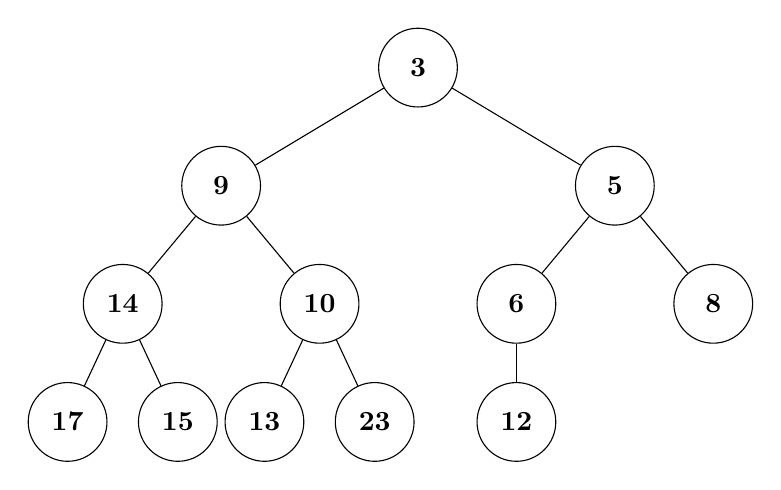
\begin{tikzpicture}[
  every node/.style={
    circle, draw, minimum size=1cm,
    font=\bfseries, inner sep=2pt
  },
  level 1/.style={sibling distance=5cm},
  level 2/.style={sibling distance=2.5cm},
  level 3/.style={sibling distance=1.4cm},
  edge from parent/.style={draw, -}
]

\node {3}
  child { node {9}
    child { node {14}
      child { node {17} }
      child { node {15} }
    }
    child { node {10}
      child { node {13} }
      child { node {23} }
    }
  }
  child { node {5}
    child { node {6}
      child { node {12} }
    }
    child { node {8} }
  };

\end{tikzpicture}
\end{center}

\item You are given the following numbers to insert into an empty Binary Search Tree (BST): $5, 7, 8, 12, 15, 27$. Determine which insertion order below would yield the tree with the least height:
\begin{enumerate}
  \item $15, 5, 27, 8, 7, 12$
  \item $12, 7, 15, 27, 5, 8$
  \item $8, 27, 7, 5, 15, 12$
  \item $7, 5, 12, 8, 15, 27$
\end{enumerate}
\mk{10}
\yr{CSE 105 | 2021--22}

%% ---------------------------------------------------------------------
%% Q3. Which insertion order gives minimum height BST?
%% ---------------------------------------------------------------------

\item A perfect balanced BST requires all interior nodes to contain two children and all leaf nodes to be on the same level. A perfect balanced BST of $h = 0$ would have $n = 1$ node, $h = 1$ would have $n = 3$ nodes, $h = 2$ would have $n = 7$ nodes, and so on. Providing appropriate arguments, derive the worst-case running time, in terms of $n$, for successfully searching for an element in a perfect balanced BST. \mk{10}
\yr{CSE 105 | 2021--22}

%% ---------------------------------------------------------------------
%% Q4. Worst-case search time in a perfect balanced BST
%% ---------------------------------------------------------------------

\item Present a recursive method \texttt{countInRange(root, low, high)}, without any helper functions, to count in a BST all keys that are within a given range. Assume keys in the BST are unique (no duplicates). For example, if the keys in a BST are $4, 7, 10, 14, 15, 17, 20, 30$, then \texttt{countInRange(root, 8, 17)} returns $4$ and \\\texttt{countInRange(root, 21, 29)} returns $0$.
For your convenience a code snippet in C++is given below , but you need not follow any particular programming language . \mk{10}
\yr{CSE 105 | 2021--22}

\begin{lstlisting}[style=javastyle]
public class BSTNode {
    int key;
    Value value;
    BSTNode left;
    BSTNode right;
    ...
}
// counts number of keys in BST that are in the range low to high, inclusive
// i.e. all keys k such that low <= k <= high
public static int countInRange(BSTNode root, int low, int high) {
    // COMPLETE THIS METHOD
}
\end{lstlisting}

%% ---------------------------------------------------------------------
%% Q5. countInRange(root, low, high) --- recursive BST method
%% ---------------------------------------------------------------------

\item Present an algorithm to delete a full node in a binary search tree. Explain how it works with illustrative examples. \mk{10}
\yr{CSE 105 | 2021--22}
%% ---------------------------------------------------------------------
%% Q6. Delete a full node from BST (node with two children)
%% ---------------------------------------------------------------------

\item Consider the following array $A$ of integers:(index start from 1)
\[ A = [16,\ 4,\ 10,\ 7,\ 14,\ 9, \ 3, \ 2,\ 8,\ 1] \]
Verify whether the array is a max heap. Derive the complexity of your verification algorithm. Justify whether the algorithm \texttt{max\_heapify(A, i)} will establish the max heap property of the array if applied with index $i = 2$. Analyze the time complexity of the \texttt{max\_heapify} algorithm. \mk{20}
\yr{CSE 105 | 2021--22}
%% ---------------------------------------------------------------------
%% Q7. A=[16,4,10,7,14,9,3,2,8,1]: verify max-heap; max_heapify(A,2)
%% ---------------------------------------------------------------------

\item Calculate the number of swap operations (data interchanges) required if you apply the \texttt{Build\_Max\_Heap} algorithm on the array $A = \{5, 3, 17, 10, 84, 19, 6, 22, 9\}$. Justify whether the max heap produced can be used as a priority queue. Show that \texttt{Heap\_Extract\_Max} algorithm is essentially a part of Heapsort. Derive and compare the time complexities of Heapsort and \texttt{Heap\_Extract\_Max}. \mk{17}
\yr{CSE 105 | 2021--22}
%% ---------------------------------------------------------------------
%% Q8. Build_Max_Heap on {5,3,17,10,84,19,6,22,9} --- swap count,
%%     priority queue justification, Heapsort, complexity comparison
%% ---------------------------------------------------------------------

\item You are given two balanced binary search trees with $m$ and $n$ elements respectively. Write a function that merges them into a balanced BST in $O(m+n)$ time. \mk{15}
\yr{CSE 203 | 2021--22}

\item Calculate for the min heap shown in the given figure. Show the resulting min heap after deleting the minimum element (10), including intermediate steps. \mk{10}
\yr{CSE 203 | 2021--22}

\begin{center}
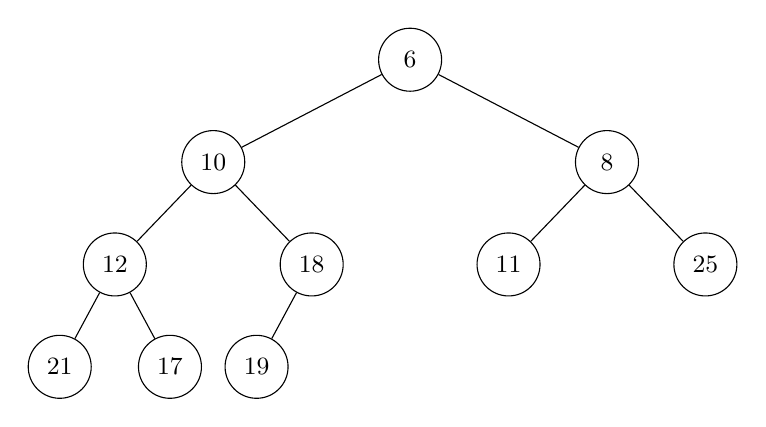
\begin{tikzpicture}[
  every node/.style={circle, draw, minimum size=8mm, font=\small},
  level distance=13mm,
  level 1/.style={sibling distance=50mm},
  level 2/.style={sibling distance=25mm},
  level 3/.style={sibling distance=14mm}
]
\node {6}
  child { node {10}
    child { node {12}
      child { node {21} }
      child { node {17} }
    }
    child { node {18}
      child { node {19} }
      child[missing] {}
    }
  }
  child { node {8}
    child { node {11} }
    child { node {25} }
  };
\end{tikzpicture}
\end{center}
%% ---------------------------------------------------------------------
%% Q: Delete min (6) from given min-heap; show steps.
%%    [CSE 203 | 2021--22]  ← Python verified \checkmark{}
%% ---------------------------------------------------------------------

\item While preparing for this exam, you have found an interesting question in a
very old book with missing pages. It talks about a Binary Search Tree (BST) that
stores integers in the range from 1 to 100 and proposes to search 22 and print
the values encountered on the search path through the BST. Then it provides the
following sequences of numbers (Sequences 1--3) and asks the following question:
``Are these sequences possible search paths through the BST?''
\begin{itemize}
  \item[] Sequence 1 : $100,\ 40,\ 20,\ 30,\ 23,\ 35,\ 22$
  \item[] Sequence 2 : $100,\ 35,\ 15,\ 32,\ 20,\ 22$
  \item[] Sequence 3 : $50,\ 60,\ 90,\ 40,\ 75$
\end{itemize}
You have to answer the above question. If your answer is `yes', please show the
path (with branches); if `no', explain why.

\textit{[Hint: you were thinking whether there was a missing page with a figure
showing the BST, but your genius little brother smiled and hinted that no need to
check for a figure as the answer lied already within the sequences provided.]}
\mk{9}
\yr{CSE 203 | 2020--21}

%% ---------------------------------------------------------------------
%% Q: BST search path validity --- Sequences 1, 2, 3
%% ---------------------------------------------------------------------

\item In a Binary Search Tree (BST), the successor of a node $N$ is defined as
the node $N_{suc}$ with the smallest key greater than the key of $N$. Similarly,
the predecessor of $N$ is defined as the node $N_{pre}$ with the largest key
smaller than the key of $N$. Now answer the following questions~(i)--(iii):
\begin{enumerate}[label=(\roman*)]
  \item Write an efficient algorithm that will store the keys of the successor
  and predecessor of each node. Assume that you have two variables, \texttt{suc}
  and \texttt{pre}, respectively in the node class/data structure for that
  purpose. \mk{7}

  \item Discuss an efficient implementation strategy of
  \texttt{removeFullNode($N$, $N_{suc}$)} (as defined below) with the help of
  appropriate illustrative examples. Analyze the time complexity of your
  strategy.
  \begin{center}
  \begin{tabular}{|p{4cm}|p{7cm}|}
  \hline
  \texttt{removeFullNode($N$, $N_{suc}$)} & $N$ is a full node that has to be
  removed from the BST. $N_{suc}$ is the successor of $N$. \\
  \hline
  \end{tabular}
  \end{center}
  \mk{12}

  \item Your genius little brother suggests that an equivalent strategy is
  available if we use $N_{pre}$ instead of $N_{suc}$. Do you agree with him?
  Justify your answer using the same illustrative example you showed in
  part~2.b(ii). \mk{7}
\end{enumerate}
\yr{CSE 203 | 2020--21}

\item Assume that a binary heap is stored in an array called \texttt{treeNodes},
which has a capacity of 100 array elements, with array index 0 not being used.
If the binary heap currently contains 86 keys, answer the following questions
with proper explanation:
\begin{enumerate}[label=(\roman*)]
  \item Is \texttt{treeNodes[44]} a leaf node?
  \item How many children does \texttt{treeNodes[43]} have?
  \item Is the subtree rooted at \texttt{treeNodes[8]} a full binary tree?
  \item How many levels are there in the subtree rooted at \texttt{treeNodes[8]}
  including \texttt{treeNodes[8]}?
  \item Including the root node (\texttt{treeNodes[1]}), how many levels are
  there in the binary heap?
  \item How many leaf nodes are there?
\end{enumerate}
\mk{12}
\yr{CSE 203 | 2020--21}

%% ---------------------------------------------------------------------
%% Q: Heap array index questions (n=86, 1-indexed).
%%    Python verified \checkmark{}
%% ---------------------------------------------------------------------

\item Show the steps of building a max-heap by inserting the numbers $45, 36, 27, 14, 86, 19, 69, 10$ one by one. Show the memory representation of the heap. Then write down the steps of sorting these numbers using heap sort. Show the analysis of how \texttt{Build-Max-Heap} can be done in $\Theta(n)$ time. \mk{10+5+10+10}
\yr{CSE 203 | 2019--20}
%% ---------------------------------------------------------------------
%% Q: Build max-heap for 45,36,27,14,86,19,69,10; heap sort.
%%    [CSE 203 | 2019--20]  ← Python verified \checkmark{}
%% ---------------------------------------------------------------------

\item Assume you are given a Max Priority Queue of $n$ elements. Write a function that first finds and then deletes the minimum element of the priority queue. \mk{10}
\yr{CSE 203 | 2018--19}

\item Consider the following max-heap of letters:

\begin{center}
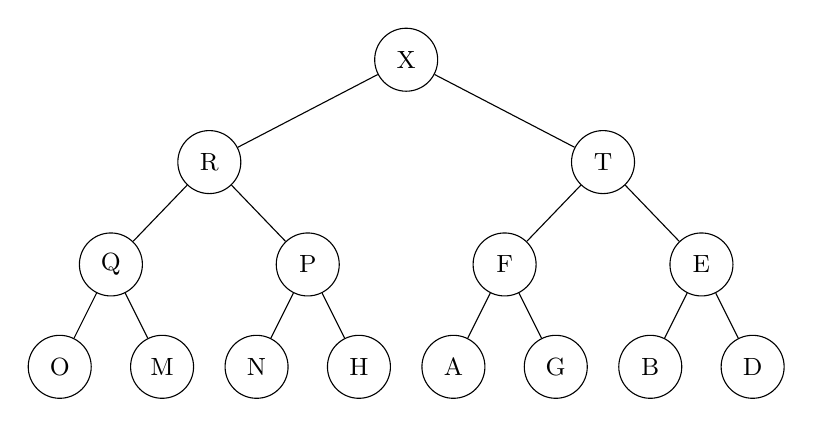
\begin{tikzpicture}[
  every node/.style={circle, draw, minimum size=8mm, font=\small},
  level distance=13mm,
  level 1/.style={sibling distance=50mm},
  level 2/.style={sibling distance=25mm},
  level 3/.style={sibling distance=13mm}
]
\node {X}
  child { node {R}
    child { node {Q}
      child { node {O} }
      child { node {M} }
    }
    child { node {P}
      child { node {N} }
      child { node {H} }
    }
  }
  child { node {T}
    child { node {F}
      child { node {A} }
      child { node {G} }
    }
    child { node {E}
      child { node {B} }
      child { node {D} }
    }
  };
\end{tikzpicture}
\end{center}

Draw the results of inserting $S$ into the above max-heap. \mk{7}
\yr{CSE 203 | 2018--19}

%% ---------------------------------------------------------------------
%% Q: Insert S into max-heap.  <- CORRECTED
%% ---------------------------------------------------------------------

\item Suppose you have a set of numbers where you do a constant number of insertions and a linear number of lookups of the maximum over some time period. Compare using a heap vs.\ a binary search tree for maintaining this set:
\begin{enumerate}
  \item What is the asymptotic upper bound on the \emph{average-case} runtime for each, and which structure should you choose?
  \item What is the asymptotic upper bound on the \emph{worst-case} runtime for each, and which structure should you choose?
\end{enumerate}
\mk{12}
\yr{CSE 203 | 2018--19}
%% ---------------------------------------------------------------------
%% Q: Heap vs BST --- constant inserts, linear max lookups.
%%    [CSE 203 | 2018--19]
%% ---------------------------------------------------------------------

\item Write a function \texttt{int treeHeight()} for a Binary Search Tree that computes the height of the tree. Give a worst-case Big-$O$ running time in terms of $n$. \mk{8}
\yr{CSE 203 | 2018--19}

\item Write a function \texttt{void deleteMax()} for a Binary Search Tree that deletes the maximum element (or does nothing if the tree is empty). Give a worst-case Big-$O$ running time in terms of $n$. Do not assume the tree is balanced. \mk{7}
\yr{CSE 203 | 2018--19}

\item Write a method \texttt{isHeap()} that determines whether a particular binary tree is a heap. What is the Big-$O$ bound on the running time of this algorithm? \mk{8}
\yr{CSE 203 | 2018--19}
%% ---------------------------------------------------------------------
%% Q: treeHeight(); deleteMax(); isHeap().  [CSE 203 | 2018--19]
%% ---------------------------------------------------------------------

\item Construct a max-heap with the data $[6, 1, 7, 2, 8, 3, 9, 4, 10, 5, 11, 17, 4, 5]$ by insertion and adjustment. Show the changes in values at each step. Carry out complexity analysis for both algorithms. \mk{5+5+10}
\yr{CSE 203 | 2017--18}

%% ---------------------------------------------------------------------
%% Q: Build max-heap from [6,1,7,2,8,3,9,4,10,5,11,17,4,5].
%%    [CSE 203 | 2017--18]  ← Python verified \checkmark{}
%% ---------------------------------------------------------------------

\item By writing a procedure, explain the three cases that may arise for deleting a node from a binary search tree. \mk{15}
\yr{CSE 203 | 2016--17, 2015--16}
%% ---------------------------------------------------------------------
%% Q: Three cases of BST deletion.  [CSE 203 | 2015--16 & 2016--17]
%% ---------------------------------------------------------------------

\item Write a function to find the smallest element in a max binary heap. \mk{8}
\yr{CSE 203 | 2016--17}

\item Write the differences between a standard queue and a priority queue. Write two functions that implement the \textsc{Decrease-Key} and \textsc{Increase-Key} operations in a max-heap. \mk{10}
\yr{CSE 203 | 2016--17}
%% ---------------------------------------------------------------------
%% Q: Queue vs PQ; Decrease-Key & Increase-Key.  [CSE 203 | 2016--17]
%% ---------------------------------------------------------------------

\item Write an algorithm that sorts the keys of a binary search tree. Draw the BST that results after inserting the keys $43, 34, 48, 59, 65, 73, 88, 81, 92, 79$ (in that order) into an initially empty BST. Also draw a BST of height three using these keys. \mk{10}
\yr{CSE 203 | 2016--17}

\item Write a function to find the largest element in a min binary heap. Assume the array representing a min binary heap contains the values $2, 8, 3, 10, 16, 7, 18, 13, 15$. Show the contents of the array after deleting the minimum element. \mk{10}
\yr{CSE 203 | 2015--16}

\item Prove that a min binary heap can be built in linear time. \mk{10}
\yr{CSE 203 | 2015--16}
%% ---------------------------------------------------------------------
%% Q: Prove min-heap built in linear time.  [CSE 203 | 2015--16]
%% ---------------------------------------------------------------------

\item Write two procedures for finding the successor element and the predecessor element in a binary search tree. \mk{10}
\yr{CSE 203 | 2015--16}
%% ---------------------------------------------------------------------
%% Q: Successor and predecessor in BST.  [CSE 203 | 2015--16]
%% ---------------------------------------------------------------------

\item What are the main operations of a priority queue? Explain how one can implement these operations using a heap. \mk{15}
\yr{CSE 203 | 2014--15, 2011--12}
%% ---------------------------------------------------------------------
%% Q: Main operations of a priority queue; implement using a heap.
%%    [CSE 203 | 2011--12]
%% ---------------------------------------------------------------------

\item Write an algorithm for building a heap. Show that an $n$-element heap can be built in $O(n)$ time. \mk{10}
\yr{CSE 203 | 2014--15}
%% ---------------------------------------------------------------------
%% Q: Build heap; show O(n).  [CSE 203 | 2014--15]
%% ---------------------------------------------------------------------

\item Draw the binary search tree that results after successively inserting the keys $15, 8, 24,\\ 12, 40, 18, 20, 23$ into an initially empty BST. Then, by using necessary rotations, redraw the BST so that it becomes an AVL tree. \mk{10}
\yr{CSE 203 | 2014--15}
%% ---------------------------------------------------------------------
%% Q: Build BST for 15,8,24,12,40,18,20,23; convert to AVL.
%%    [CSE 203 | 2014--15]
%% ---------------------------------------------------------------------

\item Suppose we create a binary search tree by inserting the following values in the given order: $50, 10, 13, 45, 55, 110, 5, 31, 64, 47$. Answer the following questions:
\begin{enumerate}
  \item Draw the binary search tree.
  \item Show the output values if we visit the tree using pre-order traversal.
  \item Show the output values if we visit the tree using post-order traversal.
  \item Show the resulting trees after deleting $47$, $110$, and $50$ (each deletion applied on the original tree).
\end{enumerate}
\mk{5+4+4+6=19}
\yr{CSE 203 | 2014--15}

%% ---------------------------------------------------------------------
%% Q: BST for 50,10,13,45,55,110,5,31,64,47; traversals; deletions.
%%    [CSE 203 | 2014--15] 
%% ---------------------------------------------------------------------

\item Give the idea of a data structure that can be used to implement a general tree where nodes can have more than two children. Re-draw the following binary search tree using your proposed data structure:
\begin{center}
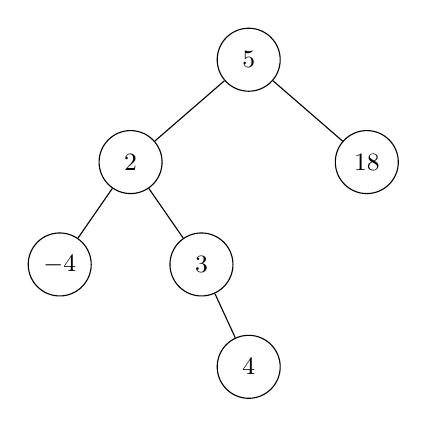
\begin{tikzpicture}[
  every node/.style={circle, draw, minimum size=8mm, font=\small},
  level distance=13mm,
  level 1/.style={sibling distance=30mm},
  level 2/.style={sibling distance=18mm},
  level 3/.style={sibling distance=12mm}
]
\node {5}
  child { node {2}
    child { node {$-4$} }
    child { node {3}
      child[missing] {}
      child { node {4} }
    }
  }
  child { node {18} };
\end{tikzpicture}
\end{center}
\mk{8}
\yr{CSE 203 | 2014--15}

\item Assume an object which has two elements \{key, element\}. An array of such objects is given. Then:
\begin{enumerate}
  \item Convert the array into a Max-heap.
  \item Insert $(36, B)$ in the resultant Max-heap.
  \item Show each step of Heap Sort over the resultant Max-heap.
\end{enumerate}
Array: $[14/U,\ 11/E,\ 13/T,\ 12/C,\ 26/S,\ 19/E,\ 20/W,\ 24/P,\ 18/O,\ 17/L,\ 7/A,\ 8/S,\\\ 9/H,\ 10/I]$
\mk{8+8+6=22}
\yr{CSE 203 | 2013--14}

\item Write down two algorithms for constructing a max-heap and deduce their complexities. Discuss how Carlsson reduces the leading coefficient in the complexity of the Heapsort algorithm. \mk{10}
\yr{CSE 207 | 2013--14}

\item Write the differences between a standard queue and a priority queue. Write the property of a Max-Heap. Write an algorithm for building a Max-Heap. Analyze the time complexity of the algorithm. \mk{3+3+7+7=20}
\yr{CSE 203 | 2012--13}
%% ---------------------------------------------------------------------
%% Q: Queue vs priority queue; Max-Heap property; Build-Max-Heap.
%%    [CSE 203 | 2012--13]
%% ---------------------------------------------------------------------

%% ---------------------------------------------------------------------
\item Sort the array $[15, 13, 9, 5, 12, 8, 7, 4, 10, 6, 2, 1, 26, 23]$ using Heapsort, showing the values at the right of the nodes at each step. \mk{8}
\yr{CSE 203 | 2011--12}

\item What is a priority queue? Write three applications of a priority queue. \mk{2+3=5}
\yr{CSE 203 | 2011--12}

%% ---------------------------------------------------------------------
%% Q10. Priority queue: definition + 3 applications
%% ---------------------------------------------------------------------

\item Explain the insertion and deletion operations in a binary search tree with illustrative examples. \mk{14}
\yr{CSE 203 | 2011--12}
%% ---------------------------------------------------------------------
%% Q: BST insertion and deletion with examples.  [CSE 203 | 2011--12]
%% ---------------------------------------------------------------------

\end{enumerate}
\newpage

\secdivider{Graphs \& Graph Representations}{Adjacency Matrix, Adjacency List, Graph Properties}{cG}{cG}
\markboth{T7 --- Graphs \& Graph Representations}{}
\label{sec:T7}
\section{T7 --- Graphs \& Graph Representations}

\begin{enumerate}
\item Given a graph $G = (V, E)$ with unique edge weights, let $(S, V-S)$ be a cut in $G$ such that $S$ is non-empty and $S \neq V$. Show that the minimum weighted crossing edge between any such cut in $G$ is included in every minimum spanning tree. \mk{15}
\yr{CSE 105 | 2023--24}
%% ---------------------------------------------------------------------
%% Q: Prove minimum crossing edge of any cut is in every MST.
%%    [CSE 105 | 2023--24]
%% ---------------------------------------------------------------------

\item Given an adjacency list representation of a directed graph $G = (V, E)$, sketch an efficient algorithm to find its transpose graph $G^T = (V, E^T)$ where $E^T = \{(v, u) \in V \times V : (u, v) \in E\}$. Analyze the time complexity of your algorithm. Also evaluate how long it takes to compute the in-degree and out-degree of every vertex of $G$. \mk{18}
\yr{CSE 105 | 2022--23}
%% ---------------------------------------------------------------------
%% Q: Transpose graph algorithm; in-degree and out-degree.
%%    [CSE 105 | 2022--23]
%% ---------------------------------------------------------------------

\item A DAG is given to you. Find the maximum number of edges that can be added to this DAG such that the resulting graph is still a DAG (i.e., adding even one more edge would create a cycle). \mk{10}
\yr{CSE 203 | 2021--22}
%% ---------------------------------------------------------------------
%% Q: Max edges addable to a DAG keeping it acyclic.
%%    [CSE 203 | 2021--22]
%% ---------------------------------------------------------------------

\item Consider the adjacency matrix representation of a directed graph $G$. Draw the graph and find its adjacency list representation considering the vertices in ascending order. Find the shortest path distance of every vertex from vertex 1 using BFS. Show the queue status when vertex 10 is just enqueued. Prove that the distance of the most recent vertex (tail in the queue) is at most one larger than the distance of the oldest vertex (head in the queue). \mk{20}
\yr{CSE 105 | 2021--22}

\[
\begin{array}{c|cccccccccc}
  & 1 & 2 & 3 & 4 & 5 & 6 & 7 & 8 & 9 & 10 \\
\hline
1  & 0 & 0 & 1 & 0 & 0 & 0 & 1 & 0 & 1 & 0 \\
2  & 0 & 0 & 0 & 0 & 1 & 0 & 0 & 0 & 0 & 0 \\
3  & 0 & 0 & 0 & 0 & 0 & 1 & 0 & 0 & 0 & 0 \\
4  & 1 & 0 & 0 & 0 & 0 & 0 & 0 & 1 & 0 & 0 \\
5  & 0 & 0 & 0 & 0 & 0 & 0 & 0 & 0 & 1 & 0 \\
6  & 0 & 0 & 0 & 0 & 0 & 0 & 1 & 0 & 0 & 0 \\
7  & 0 & 0 & 1 & 0 & 0 & 0 & 0 & 0 & 0 & 0 \\
8  & 0 & 0 & 0 & 0 & 0 & 0 & 0 & 0 & 0 & 1 \\
9  & 0 & 1 & 0 & 1 & 0 & 0 & 0 & 0 & 0 & 1 \\
10 & 0 & 0 & 0 & 0 & 0 & 0 & 0 & 1 & 0 & 0 \\
\end{array}
\]

%% ---------------------------------------------------------------------
%% Q: Adjacency matrix $\rightarrow$ graph + adjacency list; BFS distances from 1;
%%    queue state when 10 enqueued; prove distance property.
%%    [CSE 105 | 2021--22]   ← Python verified \checkmark{}
%% ---------------------------------------------------------------------

\item Write a Graph (directed) data structure using a linked list. Write a delete-node operation for the data structure. \mk{8+7}
\yr{CSE 203 | 2019--20}
%% ---------------------------------------------------------------------
%% Q: Directed graph using linked list; delete-node operation.
%%    [CSE 203 | 2019--20]
%% ---------------------------------------------------------------------

\item Suppose you are going to represent a very dense graph and want to optimize both space and time for accessing an edge. Which representation (adjacency list or adjacency matrix) would you prefer? Justify your answer. \mk{7}
\yr{CSE 203 | 2017--18}
%% ---------------------------------------------------------------------
%% Q: Dense graph --- which representation to prefer?
%%    [CSE 203 | 2017--18]
%% ---------------------------------------------------------------------

\item Compare adjacency matrix and adjacency list representations of a graph. \mk{10}
\yr{CSE 203 | 2016--17 ,2013--14}

%% ---------------------------------------------------------------------
%% Q: Compare adjacency matrix vs adjacency list.
%%    [CSE 203 | 2016--17 and 2013--14]
%% ---------------------------------------------------------------------

\item Define graph, path, cycle, and subgraph with examples. \mk{10}
\yr{CSE 203 | 2015--16}
%% ---------------------------------------------------------------------
%% Q: Define graph, path, cycle, subgraph with examples.
%%    [CSE 203 | 2015--16]
%% ---------------------------------------------------------------------

\item For each of the following operations in an undirected graph, find the worst-case running times in Big-O notation using (i) an adjacency matrix and (ii) an adjacency list:
\begin{enumerate}
  \item Determine whether a given vertex is connected to no other vertex.
  \item Determine whether the graph has a vertex that is connected to no other vertex.
  \item Determine whether a given vertex is connected to every other vertex. Give the idea of your algorithm for the adjacency list case.
\end{enumerate}
\mk{4+4+6=14}
\yr{CSE 203 | 2014--15}
%% ---------------------------------------------------------------------
%% Q: Worst-case running times for graph operations.
%%    [CSE 203 | 2014--15]
%% ---------------------------------------------------------------------

\item Give a brief description of: (i) Graph, (ii) Forest, (iii) Tree, (iv) Spanning subgraph. \mk{1.5+1.5+1.5+2.5=7}
\yr{CSE 203 | 2013--14}
%% ---------------------------------------------------------------------
%% Q: Definitions --- Graph, Forest, Tree, Spanning subgraph.
%%    [CSE 203 | 2013--14]
%% ---------------------------------------------------------------------

\item Show the adjacency matrix and adjacency list for the following graph.
Calculate the number of bytes required in both representations. Assume that the
storage requirement of a pointer and an integer is 4 bytes.

\begin{figure}[h]
  \centering
  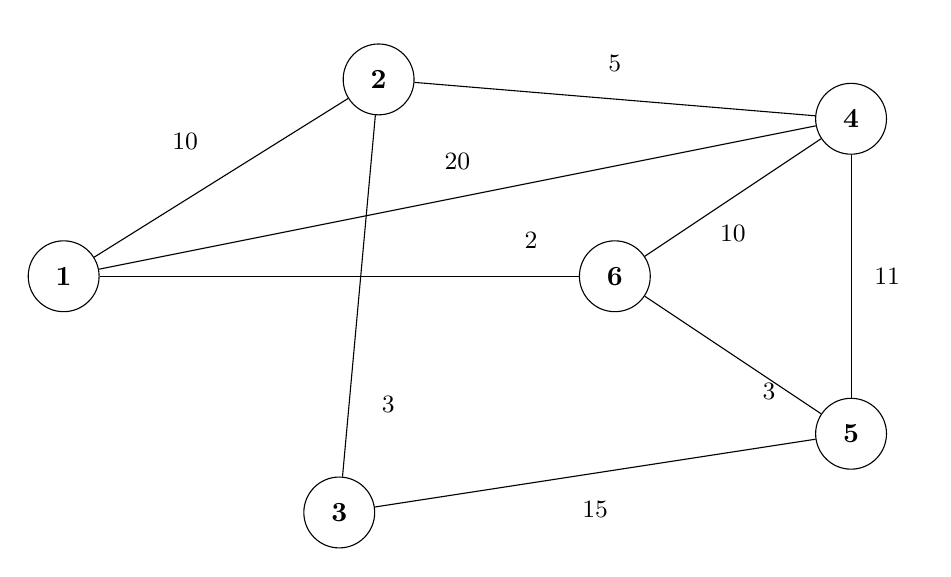
\begin{tikzpicture}[
    every node/.style={circle, draw, minimum size=0.9cm, font=\bfseries},
    edge label/.style={rectangle, draw=none, font=\normalfont\small},
    node distance=2.5cm
  ]

  % Nodes
  \node (1) at (0, 0)    {1};
  \node (2) at (4, 2.5)  {2};
  \node (3) at (3.5, -3) {3};
  \node (4) at (10, 2)   {4};
  \node (5) at (10, -2)  {5};
  \node (6) at (7, 0)    {6};

  % Edges with weights (no circle around numbers)
  \draw (1) -- node[edge label, above left]  {10} (2);
  \draw (1) -- node[edge label, above]       {20} (4);
  \draw (1) -- node[edge label,pos=0.9 ,above ]       {2}  (6);
  \draw (2) -- node[edge label, above]       {5}  (4);
  \draw (2) -- node[edge label,pos=0.7 ,below right] {3}  (3);
  \draw (3) -- node[edge label, below]       {15} (5);
  \draw (4) -- node[edge label, below]       {10} (6);
  \draw (4) -- node[edge label, right]       {11} (5);
  \draw (5) -- node[edge label, below right] {3}  (6);

  \end{tikzpicture}
  \caption{Weighted Graph}
  \label{fig:weighted-graph}
\end{figure}

%% ---------------------------------------------------------------------
%% Q: Adjacency matrix + list for weighted graph; byte counts.
%%    [CSE 203 | 2013--14]   ← Python verified \checkmark{}
%% ---------------------------------------------------------------------

\item Your friend has employed two different traversal algorithms, \textit{Algo~I}
and \textit{Algo~II}, on a graph and shown the output in Figure~Q.5(c)-I and
Figure~Q.5(c)-II respectively. In both cases, the traversal starts at the node
shown by the block right arrow. In the output, nodes are labeled with the order
they are traversed. Identify the traversal algorithm for Figure~Q.5(c)-I and
Figure~Q.5(c)-II and justify your answer. \mk{10}

% Figure Q.5 (c)-I
\begin{center}
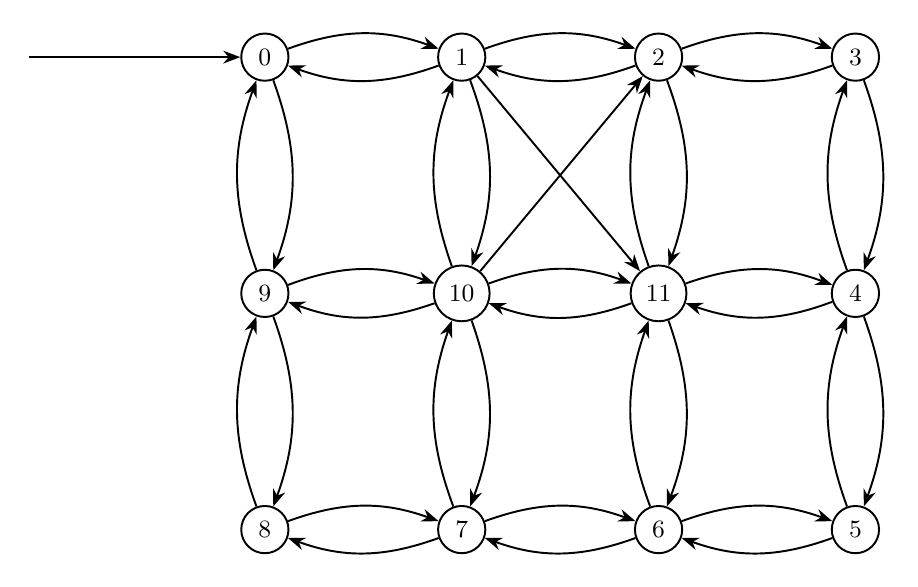
\begin{tikzpicture}[
  every node/.style={circle, draw, minimum size=0.6cm, font=\small},
  every path/.style={->, >=Stealth, line width=0.7pt},
]
\tikzset{>={Stealth[length=8pt, width=5pt]}}

% Nodes - Row 0 (top)
\node (0)  at (0,  4) {0};
\node (1)  at (2.5,4) {1};
\node (2)  at (5,  4) {2};
\node (3)  at (7.5,4) {3};

% Nodes - Row 1 (middle)
\node (9)  at (0,  1) {9};
\node (10) at (2.5,1) {10};
\node (11) at (5,  1) {11};
\node (4)  at (7.5,1) {4};

% Nodes - Row 2 (bottom)
\node (8)  at (0,  -2) {8};
\node (7)  at (2.5,-2) {7};
\node (6)  at (5,  -2) {6};
\node (5)  at (7.5,-2) {5};

% Entry arrow
\draw[->] (-3, 4) -- (0);

% Horizontal edges (top row)
\draw (0) to[bend left=20]  (1);
\draw (1) to[bend left=20]  (0);
\draw (1) to[bend left=20]  (2);
\draw (2) to[bend left=20]  (1);
\draw (2) to[bend left=20]  (3);
\draw (3) to[bend left=20]  (2);

% Horizontal edges (middle row)
\draw (9)  to[bend left=20]  (10);
\draw (10) to[bend left=20]  (9);
\draw (10) to[bend left=20]  (11);
\draw (11) to[bend left=20]  (10);
\draw (11) to[bend left=20]  (4);
\draw (4)  to[bend left=20]  (11);

% Horizontal edges (bottom row)
\draw (8)  to[bend left=20]  (7);
\draw (7)  to[bend left=20]  (8);
\draw (7)  to[bend left=20]  (6);
\draw (6)  to[bend left=20]  (7);
\draw (6)  to[bend left=20]  (5);
\draw (5)  to[bend left=20]  (6);

% Vertical edges (left col)
\draw (0)  to[bend left=20]  (9);
\draw (9)  to[bend left=20]  (0);
\draw (9)  to[bend left=20]  (8);
\draw (8)  to[bend left=20]  (9);

% Vertical edges (col 1)
\draw (10) to[bend left=20]  (1);
\draw (10) to[bend left=20]  (7);
\draw (7)  to[bend left=20]  (10);

% Vertical edges (col 2)
\draw (11) to[bend left=20]  (2);
\draw (11) to[bend left=20]  (6);
\draw (6)  to[bend left=20]  (11);
\draw (1)  to[bend left=20]  (10);
\draw (2)  to[bend left=20]  (11);
\draw (10) ->  (2);
\draw (1)  ->  (11);

% Vertical edges (right col)
\draw (3)  to[bend left=20]  (4);
\draw (4)  to[bend left=20]  (3);
\draw (4)  to[bend left=20]  (5);
\draw (5)  to[bend left=20]  (4);

\end{tikzpicture}

\end{center}
\[
 Figure Q.5(c)-I
\]

% Figure Q.5 (c)-II
\begin{center}
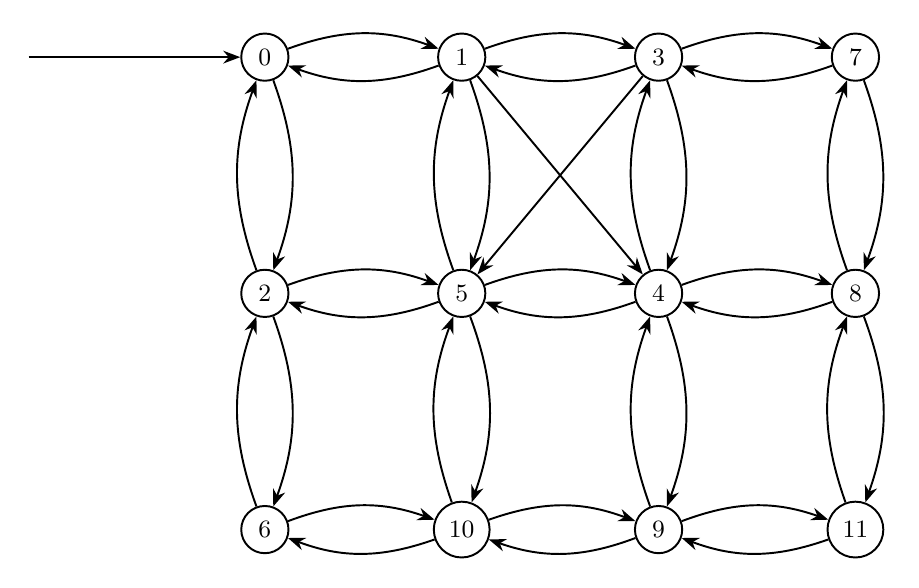
\begin{tikzpicture}[
  every node/.style={circle, draw, minimum size=0.6cm, font=\small},
  every path/.style={->, >=Stealth, line width=0.7pt},
]
\tikzset{>={Stealth[length=8pt, width=5pt]}}

% Nodes - Row 0 (top)
\node (0)  at (0,  4) {0};
\node (1)  at (2.5,4) {1};
\node (3)  at (5,  4) {3};
\node (7)  at (7.5,4) {7};

% Nodes - Row 1 (middle)
\node (2)  at (0,  1) {2};
\node (5)  at (2.5,1) {5};
\node (4)  at (5,  1) {4};
\node (8)  at (7.5,1) {8};

% Nodes - Row 2 (bottom)
\node (6)  at (0,  -2) {6};
\node (10) at (2.5,-2) {10};
\node (9)  at (5,  -2) {9};
\node (11) at (7.5,-2) {11};

% Entry arrow
\draw[->] (-3, 4) -- (0);

% Horizontal edges (top row)
\draw (0)  to[bend left=20]  (1);
\draw (1)  to[bend left=20]  (0);
\draw (1)  to[bend left=20]  (3);
\draw (3)  to[bend left=20]  (1);
\draw (3)  to[bend left=20]  (7);
\draw (7)  to[bend left=20]  (3);

% Horizontal edges (middle row)
\draw (2)  to[bend left=20]  (5);
\draw (5)  to[bend left=20]  (2);
\draw (5)  to[bend left=20]  (4);
\draw (4)  to[bend left=20]  (5);
\draw (4)  to[bend left=20]  (8);
\draw (8)  to[bend left=20]  (4);

% Horizontal edges (bottom row)
\draw (6)  to[bend left=20]  (10);
\draw (10) to[bend left=20]  (6);
\draw (10) to[bend left=20]  (9);
\draw (9)  to[bend left=20]  (10);
\draw (9)  to[bend left=20]  (11);
\draw (11) to[bend left=20]  (9);

% Vertical edges (left col)
\draw (0)  to[bend left=20]  (2);
\draw (2)  to[bend left=20]  (0);
\draw (2)  to[bend left=20]  (6);
\draw (6)  to[bend left=20]  (2);

% Vertical edges (col 1)
\draw (1)  to[bend left=20]  (5);
\draw (5)  to[bend left=20]  (1);
\draw (5)  to[bend left=20]  (10);
\draw (10) to[bend left=20]  (5);

% Vertical edges (col 2)
\draw (3)  to[bend left=20]  (4);
\draw (4)  to[bend left=20]  (3);
\draw (4)  to[bend left=20]  (9);
\draw (9)  to[bend left=20]  (4);

% Vertical edges (right col)
\draw (7)  to[bend left=20]  (8);
\draw (8)  to[bend left=20]  (7);
\draw (8)  to[bend left=20]  (11);
\draw (11) to[bend left=20]  (8);

% Cross diagonal edges
\draw (1) -> (4);
\draw (3) -> (5);

\end{tikzpicture}

\end{center}

\[
 Figure Q.5(c)-II
\]

\end{enumerate}
\newpage

\secdivider{Graph Traversals: DFS \& BFS}{DFS Algorithm, BFS Algorithm, Edge Classification}{cH}{cH}
\markboth{T8 --- Graph Traversals: DFS \& BFS}{}
\label{sec:T8}
\section{T8 --- Graph Traversals: DFS \& BFS}

\begin{enumerate}
\item Using a stack, construct an iterative (non-recursive) algorithm for
depth first search (DFS) of a graph. Show how the state of the stack changes
over time using the graph given in the figure. Analyze the complexity. Modify
the algorithm to print the type of each edge it encounters. \mk{20}
\yr{CSE 105 | 2023--24}

\begin{center}
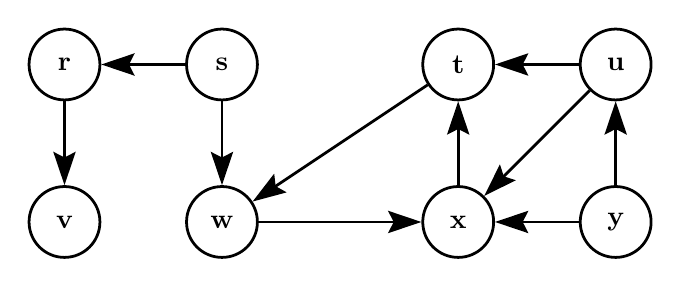
\begin{tikzpicture}[
  every node/.style={circle,draw,minimum size=0.9cm,font=\bfseries},
  every path/.style={->,line width=1pt},
]
\tikzset{>={Stealth[length=12pt,width=8pt,inset=2pt]}}
\node(r) at(0,0){r}; \node(v) at(0,-2){v};
\node(s) at(2,0){s}; \node(w) at(2,-2){w};
\node(t) at(5,0){t}; \node(x) at(5,-2){x};
\node(u) at(7,0){u}; \node(y) at(7,-2){y};
\draw(r)->(v); \draw(s)->(r); \draw(s)->(w); \draw(t)->(w);
\draw(w)->(x); \draw(u)->(t); \draw(u)->(x);
\draw(y)->(x); \draw(y)->(u); \draw(x)->(t);
\end{tikzpicture}
\end{center}

%%---------------------------------------------------------------------
\item Define the four types of edges that a DFS on a directed graph yields.
Modify the pseudocode of the original DFS algorithm to print all the edges
along with their types. Justify whether your algorithm will work correctly.
\mk{18}
\yr{CSE 105 | 2022--23}

%%---------------------------------------------------------------------
\item Classify the edges of the directed graph $G$ after running DFS on the
graph considering the vertices in ascending order. Prove that an edge $(u, v)$
is a tree edge if $u.d < v.d < v.f < u.f$. \mk{15}
\yr{CSE 105 | 2021--22}

\[
\begin{array}{c|cccccccccc}
  & 1 & 2 & 3 & 4 & 5 & 6 & 7 & 8 & 9 & 10 \\
\hline
1  & 0 & 0 & 1 & 0 & 0 & 0 & 1 & 0 & 1 & 0 \\
2  & 0 & 0 & 0 & 0 & 1 & 0 & 0 & 0 & 0 & 0 \\
3  & 0 & 0 & 0 & 0 & 0 & 1 & 0 & 0 & 0 & 0 \\
4  & 1 & 0 & 0 & 0 & 0 & 0 & 0 & 1 & 0 & 0 \\
5  & 0 & 0 & 0 & 0 & 0 & 0 & 0 & 0 & 1 & 0 \\
6  & 0 & 0 & 0 & 0 & 0 & 0 & 1 & 0 & 0 & 0 \\
7  & 0 & 0 & 1 & 0 & 0 & 0 & 0 & 0 & 0 & 0 \\
8  & 0 & 0 & 0 & 0 & 0 & 0 & 0 & 0 & 0 & 1 \\
9  & 0 & 1 & 0 & 1 & 0 & 0 & 0 & 0 & 0 & 1 \\
10 & 0 & 0 & 0 & 0 & 0 & 0 & 0 & 1 & 0 & 0 \\
\end{array}
\]

%% ---------------------------------------------------------------------
%% Q: Classify DFS edges, prove tree edge condition.
%% ---------------------------------------------------------------------

%%---------------------------------------------------------------------
\item You are given the following undirected graph to traverse using both BFS and DFS starting from vertex $u$. Show the simulation steps for labeling the vertices in order of visits. In BFS, the label of a vertex is its level; in DFS, label each vertex with its discovery and finishing times. Also write the pseudocodes for BFS and DFS. \mk{10+10}
\yr{CSE 203 | 2019--20}

\begin{center}
  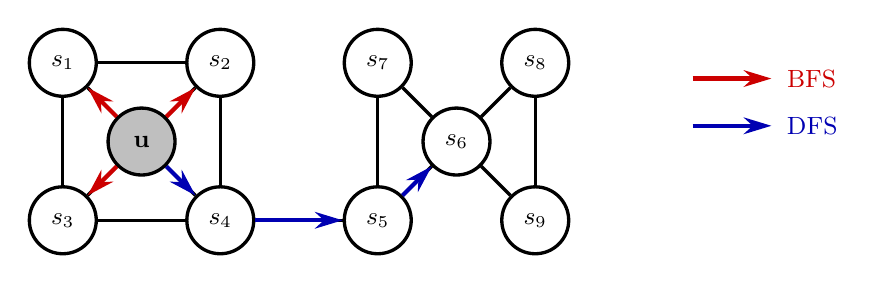
\begin{tikzpicture}[
    every node/.style={circle, draw, minimum size=0.85cm, font=\bfseries\small},
    every path/.style={line width=1.2pt},
    bfs/.style={->, color=red!80!black, line width=1.5pt},
    dfs/.style={->, color=blue!70!black, line width=1.5pt},
  ]
  \tikzset{>={Stealth[length=10pt, width=6pt]}}

  % Nodes
  \node (s1) at (0, 2)    {$s_1$};
  \node (s2) at (2, 2)    {$s_2$};
  \node[fill=gray!50]
       (u)  at (1, 1)    {u};
  \node (s3) at (0, 0)    {$s_3$};
  \node (s4) at (2, 0)    {$s_4$};
  \node (s7) at (4, 2)    {$s_7$};
  \node (s8) at (6, 2)    {$s_8$};
  \node (s5) at (4, 0)    {$s_5$};
  \node (s6) at (5, 1)    {$s_6$};
  \node (s9) at (6, 0)    {$s_9$};

  % Undirected edges (black)
  \draw (s1) -- (s2);
  \draw (s1) -- (u);
  \draw (s1) -- (s3);
  \draw (s2) -- (u);
  \draw (s2) -- (s4);
  \draw (u)  -- (s3);
  \draw (u)  -- (s4);
  \draw (s3) -- (s4);
  \draw (s4) -- (s5);
  \draw (s5) -- (s7);
  \draw (s5) -- (s6);
  \draw (s7) -- (s6);
  \draw (s8) -- (s6);
  \draw (s6) -- (s9);
  \draw (s8) -- (s9);

  % BFS arrows (red) from u
  \draw[bfs] (u) -> (s1);
  \draw[bfs] (u) -> (s3);
  \draw[bfs] (u) -> (s2);
  \draw[dfs] (u) -> (s4);

  % DFS arrows (blue)
  \draw[dfs] (s4) -> (s5);
  \draw[dfs] (s5) -> (s6);

  % Legend
  \draw[bfs] (8, 1.8) -- (9, 1.8)
    node[right, draw=none, fill=none, font=\normalfont\small] {BFS};
  \draw[dfs] (8, 1.2) -- (9, 1.2)
    node[right, draw=none, fill=none, font=\normalfont\small] {DFS};

  \end{tikzpicture}

\end{center}

\begin{center}
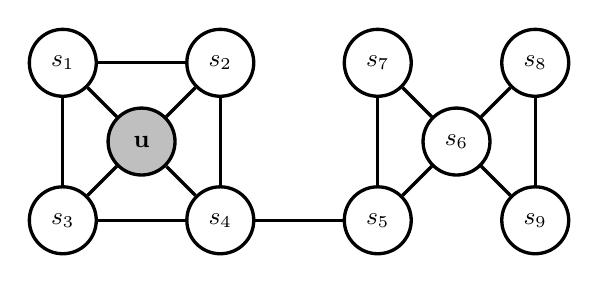
\begin{tikzpicture}[
  every node/.style={circle,draw,minimum size=0.85cm,font=\bfseries\small},
  every path/.style={line width=1.2pt},
]
\node(s1) at(0,2){$s_1$}; \node(s2) at(2,2){$s_2$};
\node[fill=gray!50](u) at(1,1){u};
\node(s3) at(0,0){$s_3$}; \node(s4) at(2,0){$s_4$};
\node(s7) at(4,2){$s_7$}; \node(s8) at(6,2){$s_8$};
\node(s5) at(4,0){$s_5$}; \node(s6) at(5,1){$s_6$};
\node(s9) at(6,0){$s_9$};
\draw(s1)--(s2); \draw(s1)--(u); \draw(s1)--(s3);
\draw(s2)--(u); \draw(s2)--(s4); \draw(u)--(s3); \draw(u)--(s4);
\draw(s3)--(s4); \draw(s4)--(s5); \draw(s5)--(s7);
\draw(s5)--(s6); \draw(s7)--(s6); \draw(s8)--(s6);
\draw(s6)--(s9); \draw(s8)--(s9);
\end{tikzpicture}
\end{center}

%% ---------------------------------------------------------------------
%% Q: BFS and DFS Simulation from u
%% ---------------------------------------------------------------------

%%---------------------------------------------------------------------
\item Explain when there is no back edge if DFS is performed on an undirected
graph. \mk{8}
\yr{CSE 203 | 2018--19}

%%---------------------------------------------------------------------
\item Give the running times of DFS using adjacency lists and adjacency matrix.
\mk{8}
\yr{CSE 203 | 2018--19}

%%---------------------------------------------------------------------
\item Would you use BFS or DFS to find any path from a start vertex to a goal
in a graph with many long paths? Justify. \mk{10}
\yr{CSE 203 | 2018--19}

%%---------------------------------------------------------------------
\item ``Given a directed graph $G$, both BFS and DFS from a particular starting vertex $s$ will traverse the same set of vertices.'' Do you agree with this statement? Justify your answer. \mk{8}
\yr{CSE 203 | 2017--18}

\item Given an undirected graph $G = (V, E)$, give a linear-time algorithm to check whether there is a cycle of odd length in the graph. Briefly justify its correctness. \mk{15}
\yr{CSE 207 | 2015--16}

%%---------------------------------------------------------------------

\item Consider the following directed graph. Answer the following questions:
\begin{enumerate}
  \item Perform depth first search on the graph starting from vertex $A$. Choose the
  smallest (in alphabetical order) vertex when there is a choice. Find the
  discovery time and finishing time of each vertex.
  \item Perform breadth first search on the graph starting from vertex $A$. Choose
  the smallest (in alphabetical order) vertex when there is a choice. Find the
  distance and parent of each vertex.
\end{enumerate}
\begin{center}
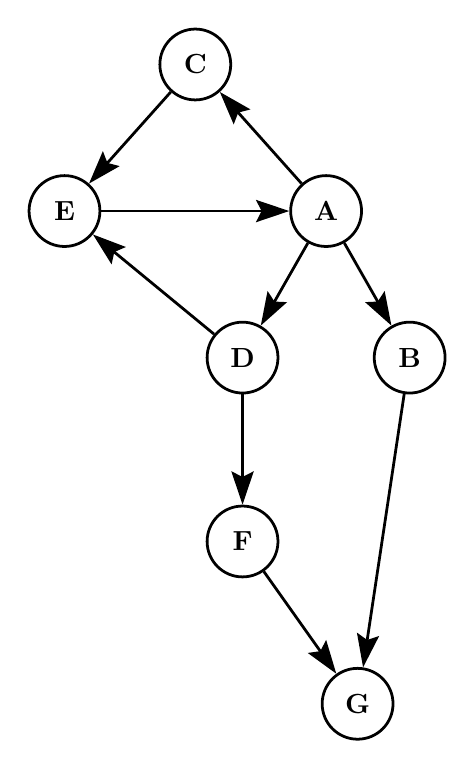
\begin{tikzpicture}[
  every node/.style={circle, draw, minimum size=0.9cm, font=\bfseries},
  every path/.style={->, line width=1pt},
]
\tikzset{>={Stealth[length=12pt, width=8pt, inset=2pt]}}
\node (C) {C};
\node (E) [below left=12mm and 10mm of C]  {E};
\node (A) [below right=12mm and 10mm of C] {A};
\node (D) [below left=12mm and 4mm of A]   {D};
\node (B) [below right=12mm and 4mm of A]  {B};
\node (F) [below=14mm of D]               {F};
\node (G) [below right=14mm and 8mm of F] {G};

\draw (C) to (E);
\draw (A) to (C);
\draw (E) to (A);
\draw (A) to (D);
\draw (A) to (B);
\draw (D) to (F);
\draw (F) to (G);
\draw (B) to (G);
\draw (D) to (E);
\end{tikzpicture}
\end{center}
\mk{6+6=12}
\yr{CSE 203 | 2014--15}

%% ---------------------------------------------------------------------
%% Q: DFS & BFS on Directed Graph
%% ---------------------------------------------------------------------

%%---------------------------------------------------------------------
\item Suggest an algorithm based on DFS that counts the number of connected
components in an undirected graph. \mk{8}
\yr{CSE 203 | 2014--15}

\item Consider the graph $G$. Perform the following:
\begin{enumerate}
  \item Write the adjacency matrix and adjacency list of graph $G$.
  \item Draw the BFS forest of graph $G$ assuming $B$ as the starting vertex.
  \item Write the sequence of vertices if you explore graph $G$ starting from vertex $B$ in DFS.
  \item Write the tree edges, back edges, forward edges, and cross edges.
\end{enumerate}
\mk{6+6+4+6=22}
\yr{CSE 203 | 2013--14}

\begin{center}
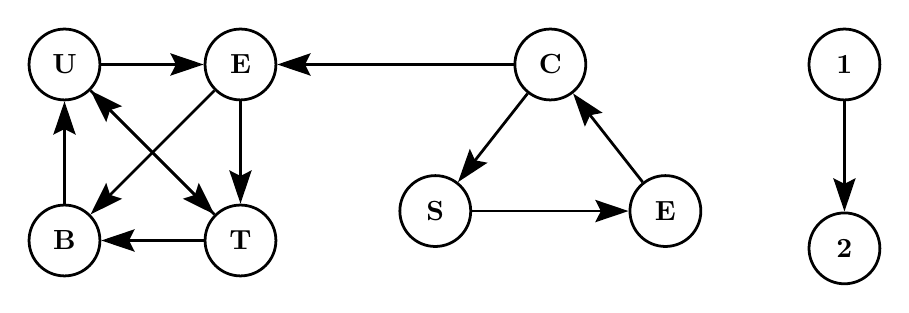
\begin{tikzpicture}[
  every node/.style={circle, draw, minimum size=0.9cm, font=\bfseries},
  every path/.style={->, line width=1pt},
]
\tikzset{>={Stealth[length=12pt, width=8pt, inset=2pt]}}

%% Graph 1
\node (U)  {U};
\node (E1) [right=13mm of U]          {E};
\node (B)  [below= 13mm of U]          {B};
\node (T)  [below= 13mm of E1]         {T};

\draw (U)  to (E1);
\draw (U)  to (T);
\draw (E1) to (B);
\draw (E1) to (T);
\draw (T)  to (B);
\draw (T)  to (U);
\draw (B)  to (U);

%% Graph 2
\node (C)  [right=30mm of E1]                  {C};
\node (S)  [below left=12mm and 8mm of C]      {S};
\node (E2) [below right=12mm and 8mm of C]     {E};

\draw (C)  to (E1);  %% C $\rightarrow$ E (Graph 1  E)
\draw (C)  to (S);
\draw (S)  to (E2);
\draw (E2) to (C);

%% Graph 3
\node (n1) [right=28mm of C]     {1};
\node (n2) [below=14mm of n1]    {2};

\draw (n1) to (n2);

\end{tikzpicture}
\end{center}

%% ---------------------------------------------------------------------
%% Q: Adjacency Matrix, BFS, DFS, and Edge Types on Graph G
%% ---------------------------------------------------------------------

\item Write an algorithm for DFS traversal. Analyze time complexity. \mk{8+7=15}
\yr{CSE 203 | 2012--13}

%%---------------------------------------------------------------------
\item Consider the graph $G$. Perform the following:
\begin{enumerate}
  \item Write the adjacency matrix and adjacency list of the graph $G$.
  \item Draw the BFS forest of the graph $G$ assuming $b$ as the starting vertex.
  \item Write the sequence of vertices if you explore the graph $G$ starting from vertex $b$ in DFS.
  \item Write the tree edges, back edges, forward edges, and cross edges.
\end{enumerate}
\mk{6+4+4+6=20}
\yr{CSE 203 | 2012--13}

\begin{center}
 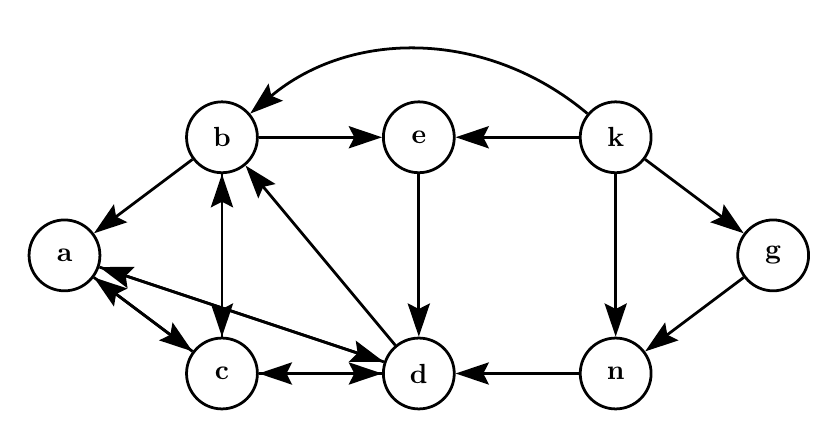
\begin{tikzpicture}[
  every node/.style={circle, draw, minimum size=0.9cm, font=\bfseries},
  every path/.style={->, line width=1pt},
]
\tikzset{>={Stealth[length=12pt, width=8pt, inset=2pt]}}

  % Nodes
  \node (a) at (0, 0)     {a};
  \node (b) at (2, 1.5)   {b};
  \node (c) at (2, -1.5)  {c};
  \node (e) at (4.5, 1.5) {e};
  \node (d) at (4.5, -1.5){d};
  \node (k) at (7, 1.5)   {k};
  \node (n) at (7, -1.5)  {n};
  \node (g) at (9, 0)     {g};

  % Edges
  \draw (b) -> (a);
  \draw (a) -> (c);
  \draw (c) -> (a);
  \draw (b) -> (c);
  \draw (c) -> (b);
  \draw (b) -> (e);
  \draw (d) -> (b);
  \draw (c) -> (d);
    \draw (d) -> (c);
  \draw (e) -> (d);
  \draw (k) -> (e);
  \draw (k) -> (n);
  \draw (k) to[bend right=40] (b);
  \draw (k) -> (g);
  \draw (n) -> (d);
  \draw (g) -> (n);
  \draw (a) -> (d);
  \draw (d) -> (a);

  \end{tikzpicture}
\end{center}

%% ---------------------------------------------------------------------
%% Q: Graph G (Adjacency Matrix, BFS, DFS, Edge Types)
%% ---------------------------------------------------------------------

%%---------------------------------------------------------------------

%%---------------------------------------------------------------------

%%---------------------------------------------------------------------
\item Write an algorithm for DFS traversal of a given graph. Analyze the time
complexity of the algorithm. \mk{10+5=15}
\yr{CSE 203 | 2011--12}

%%---------------------------------------------------------------------

\item Write the sequences of the vertices if you explore the given graph $G$ using BFS and DFS. Classify the edges of $G$ for your DFS traversal. \mk{4+6=10}
\yr{CSE 203 | 2011--12}

\begin{center}
  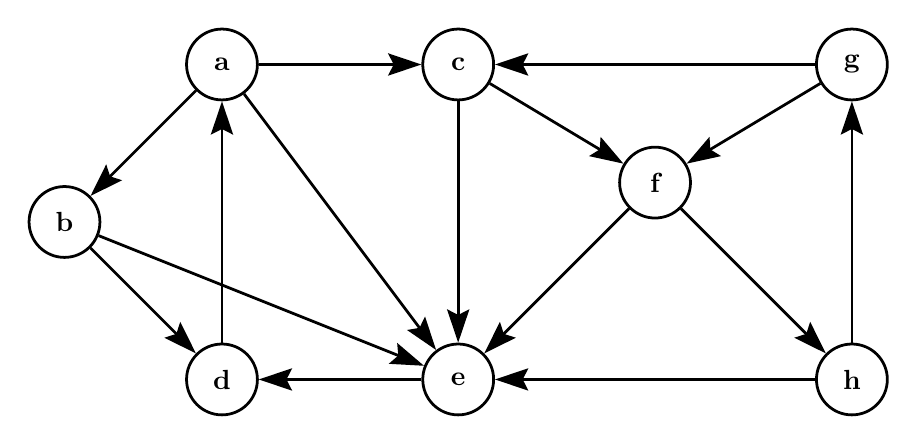
\begin{tikzpicture}[
  every node/.style={circle, draw, minimum size=0.9cm, font=\bfseries},
  every path/.style={->, line width=1pt},
]
\tikzset{>={Stealth[length=12pt, width=8pt, inset=2pt]}}

  % Nodes
  \node (b) at (0, 0)    {b};
  \node (a) at (2, 2)    {a};
  \node (d) at (2, -2)   {d};
  \node (c) at (5, 2)    {c};
  \node (e) at (5, -2)   {e};
  \node (f) at (7.5, 0.5){f};
  \node (g) at (10, 2)   {g};
  \node (h) at (10, -2)  {h};

  % Edges
  \draw (a) -> (b);
  \draw (b) -> (d);
  \draw (d) -> (a);
  \draw (a) -> (e);
  \draw (a)->(c);
  \draw (g) -> (c);
  \draw (h) -> (e);
  \draw (b) -> (e);
  \draw (e) -> (d);
  \draw (c) -> (e);
  \draw (c) -> (f);
  \draw (f) -> (e);
  \draw (g) -> (f);
  \draw (h) -> (g);
  \draw (f) -> (h);

  \end{tikzpicture}
\end{center}

%% ---------------------------------------------------------------------
%% Q: BFS & DFS on Graph G (Pure Black Diagram)
%% ---------------------------------------------------------------------

%%---------------------------------------------------------------------

%%---------------------------------------------------------------------
\item Suppose you have a graph like the one below. The dots signify some part of
the graph that you don't know exactly, not a straight link. You know however,
that there are many paths from the start to the goal. You also know that they
tend to be rather long. Suppose that you want to implement a program that
searches for a path and returns the first one it can find. You have no need for
finding the optimal path in any sense, just any path will do. Would you want to
use BFS or DFS as the basis for your program? Justify your answer.

\begin{center}
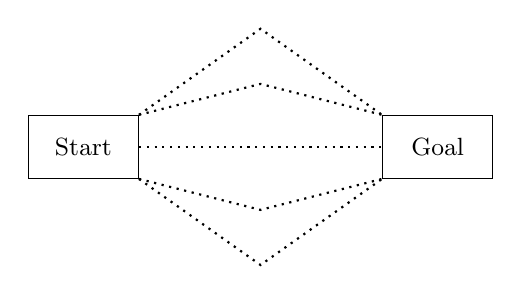
\begin{tikzpicture}[
  every node/.style={draw, minimum height=8mm, minimum width=14mm, font=\small},
  node distance=0mm
]
\node (start) at (0, 0)    {Start};
\node (goal)  at (4.5, 0)  {Goal};

\draw[dotted, thick] (start.north east) -- (2.25,  1.5) -- (goal.north west);
\draw[dotted, thick] (start.north east) -- (2.25,  0.8) -- (goal.north west);
\draw[dotted, thick] (start.east)       -- (2.25,  0)   -- (goal.west);
\draw[dotted, thick] (start.south east) -- (2.25, -0.8) -- (goal.south west);
\draw[dotted, thick] (start.south east) -- (2.25, -1.5) -- (goal.south west);
\end{tikzpicture}
\end{center}
\mk{10}

\item Consider the weighted graph $G$ as shown in Figure~1. Then draw the adjacency
lists of the weighted graph $G$. Whenever there is a choice of vertices to explore,
always pick the one that is alphabetically first.

\begin{center}
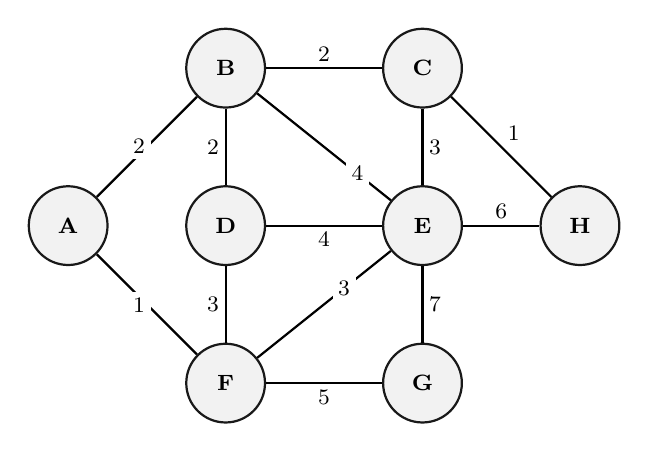
\begin{tikzpicture}[
  % নোডের নতুন এবং পরিষ্কার স্টাইল
  node/.style={circle, draw=black!90, thick, fill=gray!10, minimum size=10mm, font=\footnotesize\bfseries},
  % এজ ওয়েটের নতুন স্টাইল: বড় ফন্ট এবং সাদা ব্যাকগ্রাউন্ড
  edge_label/.style={fill=white, inner sep=2pt, font=\footnotesize, text=black}
]

% নোডগুলোর অবস্থান আগের মতোই রাখা হয়েছে
\node[node] (A) at (0,   2)   {A};
\node[node] (B) at (2,   4)   {B};
\node[node] (C) at (4.5, 4)   {C};
\node[node] (D) at (2,   2)   {D};
\node[node] (E) at (4.5, 2)   {E};
\node[node] (F) at (2,   0)   {F};
\node[node] (G) at (4.5, 0)   {G};
\node[node] (H) at (6.5, 2)   {H};

% প্রতিটি এজের অবস্থান এবং ওয়েটের প্লেসমেন্ট অপ্টিমাইজ করা হয়েছে
\draw[thick] (A) -- node[edge_label, pos=0.45, xshift=-1pt, yshift=2pt] {2} (B);
\draw[thick] (A) -- node[edge_label, pos=0.45, xshift=-1pt, yshift=-2pt] {1} (F);
\draw[thick] (B) -- node[edge_label, midway, above] {2} (C);
\draw[thick] (B) -- node[edge_label, midway, left] {2} (D);
\draw[thick] (B) -- node[edge_label, pos=0.75] {4} (E); % এই এজটি D নোডের উপর দিয়ে যায়, ওয়েট পরে দেওয়া হয়েছে
\draw[thick] (C) -- node[edge_label, midway, right] {3} (E);
\draw[thick] (C) -- node[edge_label, midway, above right] {1} (H);
\draw[thick] (D) -- node[edge_label, midway, below] {4} (E); % ওয়েট নিচে দেওয়া হয়েছে
\draw[thick] (D) -- node[edge_label, midway, left] {3} (F);
\draw[thick] (E) -- node[edge_label, pos=0.35] {3} (F); % এই এজটি D-E এবং F-G এর উপর দিয়ে যায়, ওয়েট আগে দেওয়া হয়েছে
\draw[thick] (E) -- node[edge_label, midway, right] {7} (G);
\draw[thick] (E) -- node[edge_label, midway, above] {6} (H);
\draw[thick] (F) -- node[edge_label, midway, below] {5} (G);

\end{tikzpicture}

\end{center}

\end{enumerate}
\newpage

\secdivider{Applications of DFS \& BFS}{Topological Sort, SCC, Shortest Paths, Dijkstra}{cA}{cA}
\markboth{T8a --- Applications of DFS \& BFS}{}
\label{sec:T8a}
\section{T8a --- Applications of DFS \& BFS}

\begin{enumerate}
\item Explain why the topological sort algorithm cannot run on a directed graph that contains cycle(s). Derive the component graph of the directed graph $G$ represented by the given adjacency matrix. Then find the topological sorting of the vertices of the component graph. Show every step. \mk{15}
\yr{CSE 105 | 2021--22}

\[
\begin{array}{c|cccccccccc}
  & 1 & 2 & 3 & 4 & 5 & 6 & 7 & 8 & 9 & 10 \\
\hline
1  & 0 & 0 & 1 & 0 & 0 & 0 & 1 & 0 & 1 & 0 \\
2  & 0 & 0 & 0 & 0 & 1 & 0 & 0 & 0 & 0 & 0 \\
3  & 0 & 0 & 0 & 0 & 0 & 1 & 0 & 0 & 0 & 0 \\
4  & 1 & 0 & 0 & 0 & 0 & 0 & 0 & 1 & 0 & 0 \\
5  & 0 & 0 & 0 & 0 & 0 & 0 & 0 & 0 & 1 & 0 \\
6  & 0 & 0 & 0 & 0 & 0 & 0 & 1 & 0 & 0 & 0 \\
7  & 0 & 0 & 1 & 0 & 0 & 0 & 0 & 0 & 0 & 0 \\
8  & 0 & 0 & 0 & 0 & 0 & 0 & 0 & 0 & 0 & 1 \\
9  & 0 & 1 & 0 & 1 & 0 & 0 & 0 & 0 & 0 & 1 \\
10 & 0 & 0 & 0 & 0 & 0 & 0 & 0 & 1 & 0 & 0 \\
\end{array}
\]

\item How do you determine whether a given graph is bipartite? \mk{10}
\yr{CSE 203 | 2019--20}
%% ---------------------------------------------------------------------
%% Q: Determine whether a graph is bipartite.  [CSE 203 | 2019--20]
%% ---------------------------------------------------------------------

\item Write a function to find the lexicographically smallest topological ordering of a directed graph with $N$ vertices and $M$ edges that may contain cycles. Print $-1$ if the graph has cycles. \mk{8}
\yr{CSE 203 | 2018--19}

%% ---------------------------------------------------------------------
%% Q: Lexicographically smallest topological sort; print -1 if cycle.
%%    [CSE 203 | 2018--19]   ← Python verified \checkmark{}
%% ---------------------------------------------------------------------

\item The following is Dijkstra's algorithm. Perform a line-by-line time-complexity analysis for an input graph $G$ where an adjacency list is used for graph representation and an ordinary array is used for storing $d[\,]$ values.
\begin{algorithm}[H]
\begin{algorithmic}[1]
\State $Q \gets V[G]$
\For{each $v \in Q$} 
\State $d[v] \gets \infty$ \EndFor
\State $d[s] \gets 0$; $S \gets \emptyset$
\While{$Q \neq \emptyset$}
  \State $u \gets \textsc{ExtractMin}(Q)$
  \State $S \gets S \cup \{u\}$
  \For{each $v \in u.\text{Adj}[\,]$}
    \If{$v \in Q$ and $d[v] > d[u] + w(u,v)$}
      \State $d[v] \gets d[u] + w(u,v)$
    \EndIf
  \EndFor
\EndWhile
\end{algorithmic}
\end{algorithm}
\mk{15}
\yr{CSE 207 | 2018--19}
%% ---------------------------------------------------------------------
%% Q: Line-by-line complexity of Dijkstra with adjacency list
%%    and ordinary array.  [CSE 207 | 2018--19]
%% ---------------------------------------------------------------------

\item Johnson's Algorithm uses Bellman-Ford and Dijkstra's algorithms to compute All-Pairs-Shortest-Paths efficiently on sparse graphs. Explain the basic clever idea of Johnson's Algorithm. \mk{15}
\yr{CSE 207 | 2018--19}
%% ---------------------------------------------------------------------
%% Q: Johnson's Algorithm --- basic idea.  [CSE 207 | 2018--19]
%% ---------------------------------------------------------------------

\item Briefly explain how a directed acyclic graph $G = (V, E)$ can be topologically sorted so that if $(u, v)$ is an edge then $u$ appears before $v$ in the ordering. Pseudocode is not needed. \mk{8}
\yr{CSE 203 | 2017--18}
%% ---------------------------------------------------------------------
%% Q: Topological sort of a DAG.  [CSE 203 | 2017--18]
%% ---------------------------------------------------------------------

\item Suppose you are developing a feature for Facebook. You have access to everyone's friend list and the goal is to show how any two users are connected through a chain of ``a friend of a friend''. For two users $A$ and $B$, show a sequence of individuals $X_0, X_1, \ldots, X_n$ where $X_0 = A$, $X_n = B$, and $X_i$ is friends with $X_{i+1}$, such that the length of the sequence is minimized. Explain how this can be formulated as a graph problem and what algorithm you would use. \mk{7}
\yr{CSE 203 | 2017--18}
%% ---------------------------------------------------------------------
%% Q: Facebook friend chain --- graph formulation.  [CSE 203 | 2017--18]
%% ---------------------------------------------------------------------

\item How can BFS be adapted to solve the single-source shortest path problem in an edge-weighted graph with unequal weights? Explain. \mk{8}
\yr{CSE 207 | 2017--18}
%% ---------------------------------------------------------------------
%% Q: BFS for shortest paths in edge-weighted graph.
%%    [CSE 207 | 2017--18]
%% ---------------------------------------------------------------------

\item Explain the intuitive idea behind the Bellman-Ford algorithm. How can you detect a negative cycle using Bellman-Ford? \mk{6+2}
\yr{CSE 207 | 2017--18}
%% ---------------------------------------------------------------------
%% Q: Bellman-Ford idea; negative cycle detection.
%%    [CSE 207 | 2017--18]
%% ---------------------------------------------------------------------

\item Write Dijkstra's algorithm for the single-source shortest path problem. Prove its correctness. Analyze the time complexity of the algorithm. What would be the running time if a Fibonacci heap is used instead of a binary heap? \mk{5+5+7+5}
\yr{CSE 207 | 2017--18}
%% ---------------------------------------------------------------------
%% Q: Dijkstra's algorithm; correctness; complexity; Fibonacci heap.
%%    [CSE 207 | 2017--18]
%% ---------------------------------------------------------------------

\item Design a linear-time algorithm for each of the following. Briefly describe the ideas (pseudocode is not needed):
\begin{enumerate}
  \item Given an undirected graph $G$ and a particular edge $(u, v)$ in it, determine whether $G$ has a cycle containing $(u, v)$.
  \item Given an undirected and unweighted graph $G$, a particular edge $(u, v)$, and two vertices $s$ and $t$, determine whether there is a shortest path from $s$ to $t$ containing the edge $(u, v)$.
\end{enumerate}
\mk{7+8}
\yr{CSE 203 | 2016--17}
%% ---------------------------------------------------------------------
%% Q: Linear-time algorithms --- cycle through edge; shortest path
%%    through edge.  [CSE 203 | 2016--17]
%% ---------------------------------------------------------------------

\item Write the properties satisfied by shortest paths of a graph. Show by example that Dijkstra's algorithm gives wrong results for a graph with negative-weight edges. Write an algorithm that finds shortest paths in a DAG and analyze its time complexity. \mk{15}
\yr{CSE 207 | 2016--17}
%% ---------------------------------------------------------------------
%% Q: Shortest paths properties; Dijkstra fails on negative edges;
%%    DAG shortest path algorithm.  [CSE 207 | 2016--17]
%% ---------------------------------------------------------------------

\item Prove that the Bellman-Ford algorithm returns TRUE if the input graph contains no negative-weight cycles reachable from the source, and FALSE otherwise. \mk{10}
\yr{CSE 207 | 2016--17}
%% ---------------------------------------------------------------------
%% Q: Bellman-Ford returns TRUE iff no negative cycle.
%%    [CSE 207 | 2016--17]
%% ---------------------------------------------------------------------

\item Run DFS on a given graph starting from vertex $A$ and show the discovery and finishing times for each vertex as well as the edge types. Decompose the graph into strongly connected components (SCCs). \mk{15}
\yr{CSE 203 | 2016--17}

\begin{center}
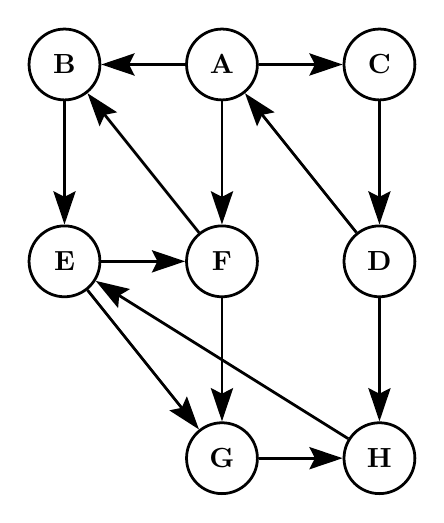
\begin{tikzpicture}[
  every node/.style={circle, draw, minimum size=0.9cm, font=\bfseries},
  every path/.style={->, line width=1pt},
]
\tikzset{>={Stealth[length=12pt, width=8pt, inset=2pt]}}
\node (A) at (2, 3)  {A};
\node (B) at (0, 3)  {B};
\node (C) at (4, 3)  {C};
\node (E) at (0, 0.5){E};
\node (F) at (2, 0.5){F};
\node (D) at (4, 0.5){D};
\node (G) at (2, -2)  {G};
\node (H) at (4, -2)  {H};

\draw (A) to (B);
\draw (D) to (A);
\draw (A) to (C);
\draw (A) to (F);
\draw (B) to (E);
\draw (C) to (D);
\draw (D) to (H);
\draw (E) to (F);
\draw (E) to (G);
\draw (F) to (G);
\draw (G) to (H);
\draw (H) to (E);
\draw (F) to (B);
\end{tikzpicture}
\end{center}

%% ---------------------------------------------------------------------
%% Q: DFS on A--H graph; discovery/finish times; edge types; SCCs.
%%    [CSE 203 | 2016--17]   ← Python verified \checkmark{}
%% ---------------------------------------------------------------------

\item Suppose a CS curriculum consists of $n$ mandatory courses. The prerequisite directed graph $G$ has a node for each course and an edge from $v$ to $w$ if $v$ is a prerequisite for $w$. Give a linear-time algorithm that computes the minimum number of semesters necessary to complete the curriculum (a student may take any number of courses per semester). \mk{15}
\yr{CSE 207 | 2015--16}
%% ---------------------------------------------------------------------
%% Q: Min semesters for CS curriculum (longest path in DAG).
%%    [CSE 207 | 2015--16]
%% ---------------------------------------------------------------------

\item Let $C$ and $C'$ be distinct strongly connected components in a directed graph $G = (V, E)$. Suppose there is an edge $(u, v) \in E$ where $u \in C$ and $v \in C'$. Prove that $f(C) > f(C')$, where $f(U)$ denotes the latest finishing time of any vertex in $U$. \mk{10}
\yr{CSE 207 | 2014--15}
%% ---------------------------------------------------------------------
%% Q: f(C) > f(C') when edge (u,v) goes from SCC C to C'.
%%    [CSE 207 | 2014--15]
%% ---------------------------------------------------------------------

\item State and prove the convergence property of edge relaxation in the context of shortest paths. \mk{8}
\yr{CSE 207 | 2014--15}

\item Provide a correctness proof of Dijkstra's algorithm. \mk{10}
\yr{CSE 207 | 2014--15}
%% ---------------------------------------------------------------------
%% Q: Correctness proof of Dijkstra's algorithm.  [CSE 207 | 2014--15]
%% ---------------------------------------------------------------------

\item Apply the Bellman-Ford algorithm to find the shortest paths. Show all relaxation steps. \mk{10}
\yr{CSE 207 | 2014--15}

\begin{center}
  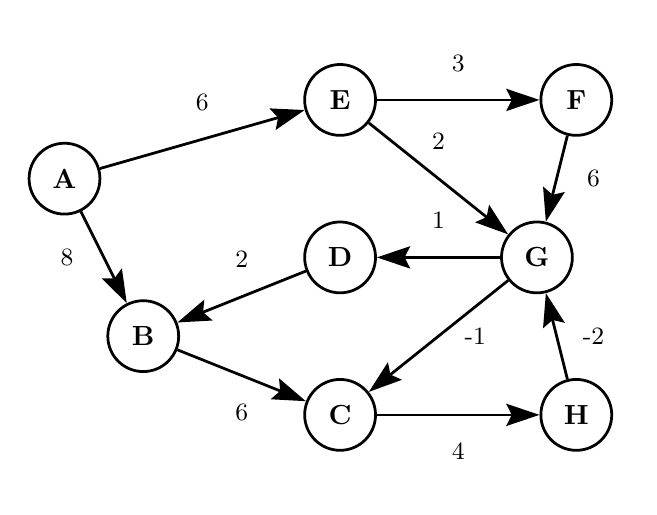
\begin{tikzpicture}[
    every node/.style={circle, draw, minimum size=0.9cm, font=\bfseries},
    edge label/.style={rectangle, draw=none, font=\normalfont\small},
  every path/.style={->, line width=1pt},
  ]
\tikzset{>={Stealth[length=12pt, width=8pt, inset=2pt]}}

  \node (A) at (0, 2)    {A};
  \node (B) at (1, 0)    {B};
  \node (C) at (3.5, -1) {C};
  \node (D) at (3.5, 1)  {D};
  \node (E) at (3.5, 3)  {E};
  \node (F) at (6.5, 3)  {F};
  \node (G) at (6, 1)    {G};
  \node (H) at (6.5, -1) {H};

  \draw (A) -> node[edge label, above] {6} (E);
  \draw (A) -> node[edge label, left]  {8} (B);
  \draw (E) -> node[edge label, above] {3} (F);
  \draw (E) -> node[edge label, above] {2} (G);
  \draw (F) -> node[edge label, right] {6} (G);
  \draw (G) -> node[edge label, above] {1} (D);
  \draw (H) -> node[edge label, right] {-2}(G);
  \draw (G) -> node[edge label, right] {-1}(C);
  \draw (D) -> node[edge label, above] {2} (B);
  \draw (B) -> node[edge label, below] {6} (C);
  \draw (C) -> node[edge label, below] {4} (H);

  \end{tikzpicture}

\end{center}

\item Find the different types of edges if DFS is applied from vertex $A$. Discuss the edges' properties with respect to the graph. \mk{6}
\yr{CSE 207 | 2014--15}

\begin{center}
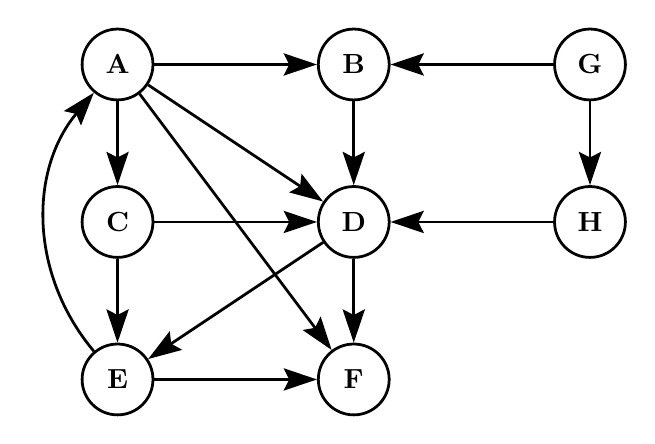
\begin{tikzpicture}[
  every node/.style={circle, draw, minimum size=0.9cm, font=\bfseries},
  every path/.style={->, line width=1pt},
]
\tikzset{>={Stealth[length=12pt, width=8pt, inset=2pt]}}

  % Nodes
  \node (A) at (0, 4)   {A};
  \node (B) at (3, 4)   {B};
  \node (G) at (6, 4)   {G};
  \node (C) at (0, 2)   {C};
  \node (D) at (3, 2)   {D};
  \node (H) at (6, 2)   {H};
  \node (E) at (0, 0)   {E};
  \node (F) at (3, 0)   {F};

  % Edges
  \draw (A) -> (B);
  \draw (A) -> (C);
  \draw (A) -> (F);
  \draw (E) to[bend left=40] (A);
  \draw (A) -> (D);
  \draw (B) -> (D);
  \draw (G) -> (H);
  \draw (H) -> (D);
  \draw (C) -> (D);
  \draw (C) -> (E);
  \draw (D) -> (E);
  \draw (D) -> (F);
  \draw (E) -> (F);
  \draw (G) -> (B);
   \end{tikzpicture}
\end{center}

\item Show the topological sorting order of a given graph with explanation of discovery and finishing times of node exploration. \mk{6}
\yr{CSE 207 | 2014--15}

\begin{center}
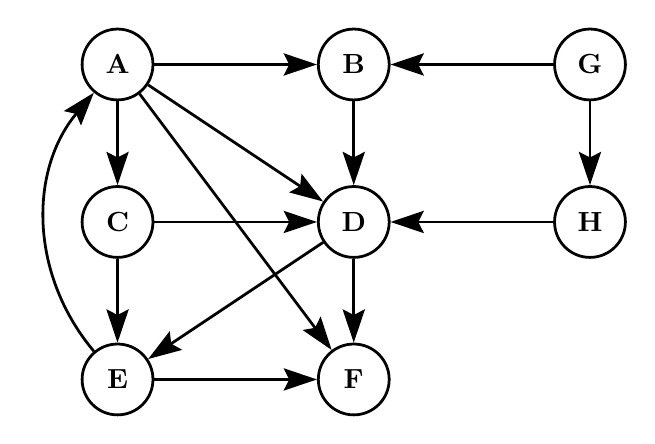
\begin{tikzpicture}[
  every node/.style={circle, draw, minimum size=0.9cm, font=\bfseries},
  every path/.style={->, line width=1pt},
]
\tikzset{>={Stealth[length=12pt, width=8pt, inset=2pt]}}

  % Nodes
  \node (A) at (0, 4)   {A};
  \node (B) at (3, 4)   {B};
  \node (G) at (6, 4)   {G};
  \node (C) at (0, 2)   {C};
  \node (D) at (3, 2)   {D};
  \node (H) at (6, 2)   {H};
  \node (E) at (0, 0)   {E};
  \node (F) at (3, 0)   {F};

  % Edges
  \draw (A) -> (B);
  \draw (A) -> (C);
  \draw (A) -> (F);
  \draw (E) to[bend left=40] (A);
  \draw (A) -> (D);
  \draw (B) -> (D);
  \draw (G) -> (H);
  \draw (H) -> (D);
  \draw (C) -> (D);
  \draw (C) -> (E);
  \draw (D) -> (E);
  \draw (D) -> (F);
  \draw (E) -> (F);
  \draw (G) -> (B);
   \end{tikzpicture}
\end{center}

\item State and prove the convergence property of shortest paths. \mk{12}
\yr{CSE 207 | 2012--13}
%% ---------------------------------------------------------------------
%% Q: Convergence property of shortest paths (state and prove).
%%    [CSE 207 | 2012--13 and 2014--15]
%% ---------------------------------------------------------------------

\item Write the Bellman-Ford algorithm. Analyze the time complexity and correctness of the Bellman-Ford algorithm. \mk{20}
\yr{CSE 207 | 2012--13}
%% ---------------------------------------------------------------------
%% Q: Bellman-Ford algorithm; time complexity; correctness.
%%    [CSE 207 | 2012--13]
%% ---------------------------------------------------------------------

\item Does Dijkstra's algorithm terminate if it is applied on a graph $G$ that contains a negative-weight cycle? Why or why not? Justify your answer. \mk{6}
\yr{CSE 207 | 2012--13}
%% ---------------------------------------------------------------------
%% Q: Does Dijkstra terminate on negative-weight cycle?
%%    [CSE 207 | 2012--13]
%% ---------------------------------------------------------------------

\item State the parenthesis theorem for depth-first search. \mk{6}
\yr{CSE 207 | 2012--13}
%% ---------------------------------------------------------------------
%% Q: Parenthesis theorem for DFS (state and prove).
%%    [CSE 207 | 2012--13 and 2014--15]
%% ---------------------------------------------------------------------

\item Assume that a breadth-first tree has already been computed with BFS on a graph $G$ with source vertex $s$. Write an algorithm to print the vertices on a shortest path from $s$ to $v$. \mk{8}
\yr{CSE 207 | 2012--13}
%% ---------------------------------------------------------------------
%% Q: Print shortest path from BFS tree.  [CSE 207 | 2012--13]
%% ---------------------------------------------------------------------

\item Prove that the component graph of a directed graph is a DAG. \mk{6}
\yr{CSE 207 | 2012--13}
%% ---------------------------------------------------------------------
%% Q: Prove component graph is a DAG.  [CSE 207 | 2012--13]
%% ---------------------------------------------------------------------

\item Write a linear-time algorithm to compute the strongly connected components of a directed graph $G = (V, E)$ using two depth-first searches. Give an example to show every step of the algorithm. \mk{8+5}
\yr{CSE 207 | 2012--13}
%% ---------------------------------------------------------------------
%% Q: Kosaraju's SCC algorithm; example.  [CSE 207 | 2012--13]
%%    Example: q,r,s,t,u,v,w,x,y,z graph  ← Python verified \checkmark{}
%% ---------------------------------------------------------------------

\item What does $d[v]$ represent at the end of the execution of Algorithm 1, if the algorithm is applied on an unweighted directed acyclic graph (DAG) $G$ with a source $s$? What is the runtime complexity in terms of $|V|$ and $|E|$ of Algorithm 1? \mk{6+6}
\yr{CSE 207 | 2012--13}

\begin{algorithm}[H]
\caption{\textsc{LongestPath-DAG}($G$)}
\begin{algorithmic}[1]
\State Compute a topological sorting of $G$
\For{each $v \in V[G]$}
    \State $d[v] \gets 0$
\EndFor
\For{each $u$ in topologically sorted order}
    \For{each $v \in Adj[u]$}
        \If{$d[v] < d[u] + 1$}
            \State $d[v] \gets d[u] + 1$
        \EndIf
    \EndFor
\EndFor
\end{algorithmic}
\end{algorithm}
 

%% ---------------------------------------------------------------------
%% Q: d[v] in DAG longest-path algorithm; runtime.
%%    [CSE 207 | 2012--13]
%% ---------------------------------------------------------------------

\item In Figure 1, the shortest path estimate of each vertex appears within the vertex and the distance to traverse from a vertex to another appears as the weight of the corresponding directed edge. Show the updated shortest path estimates of vertices after relaxing the following edges. \mk{6}

\begin{center}
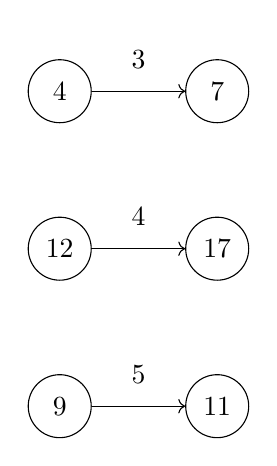
\begin{tikzpicture}[node distance=2cm, every node/.style={circle, draw, minimum size=0.8cm}]
  \node (4)  {4};
  \node (7)  [right of=4] {7};
  \node (12) [below of=4] {12};
  \node (17) [right of=12] {17};
  \node (9)  [below of=12] {9};
  \node (11) [right of=9] {11};
  \draw[->] (4)  -- node[draw=none, above] {3} (7);
  \draw[->] (12) -- node[draw=none, above] {4} (17);
  \draw[->] (9)  -- node[draw=none, above] {5} (11);
\end{tikzpicture}
\end{center}
\yr{CSE 207 | 2012--13}

\item Prove the correctness of the BFS algorithm. What are ``discovery time'' and ``finish time'' in DFS? How can you find the shortest path between two nodes from a BFS tree? \mk{8+4+6}
\yr{CSE 207 | 2009--10}
%% ---------------------------------------------------------------------
%% Q: BFS correctness; discovery/finish time in DFS; shortest path
%%    from BFS tree.  [CSE 207 | 2009--10]
%% ---------------------------------------------------------------------

\item A project is described by tasks $A, B, C, D, E, F$ taking $5, 3, 2, 2, 4, 2$ days respectively, with precedence constraints (e.g., $E$ cannot start until $C$ and $D$ are completed, but $D$ can be done in parallel with $B$ and $C$). Write a pseudocode that computes the total time required to complete the project using the PERT technique. \mk{8}
\yr{CSE 207 | 2009--10}

\begin{center}
  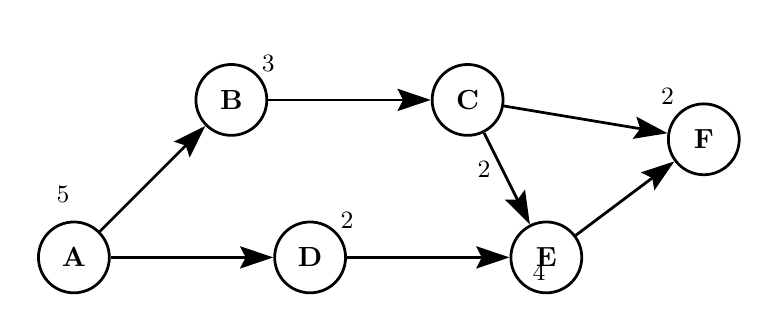
\begin{tikzpicture}[
    every node/.style={circle, draw, minimum size=0.9cm, font=\bfseries},
    edge label/.style={rectangle, draw=none, font=\normalfont\small},
  every path/.style={->, line width=1pt},
  ]
\tikzset{>={Stealth[length=12pt, width=8pt, inset=2pt]}}

  \node (A) at (0, 0)   {A};
  \node (B) at (2, 2)   {B};
  \node (C) at (5, 2)   {C};
  \node (D) at (3, 0)   {D};
  \node (E) at (6, 0)   {E};
  \node (F) at (8, 1.5) {F};

  \draw (A) -> node[edge label, pos=0,above left] {5} (B);
  \draw (A) -> (D);
  \draw (B) -> node[edge label, pos=0, above]      {3} (C);
  \draw (C) -> node[edge label, pos=0,below]      {2} (E);
  \draw (C) -> node[edge label, pos=1, above]      {2} (F);
  \draw (D) -> node[edge label, pos=0, above]      {2} (E);
  \draw (E) -> node[edge label, pos=0, below left]{4} (F);

  \end{tikzpicture}

\end{center}

\item Using DFS, compute the strongly connected components and the component graph $G^{SCC}$. Show the discovery/finish times and the DFS forests created during computation. Start alphabetically. \mk{17}
\yr{CSE 207 | 2009--10}

\begin{center}

  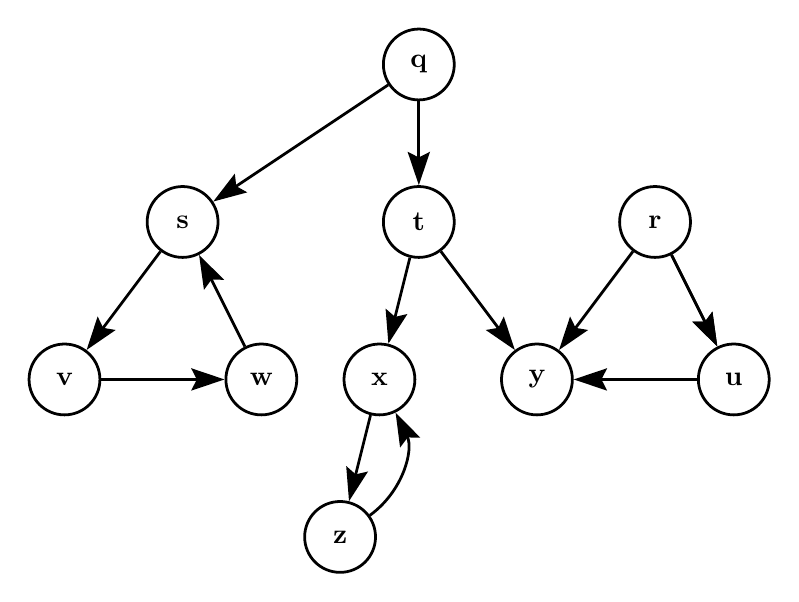
\begin{tikzpicture}[
    every node/.style={circle, draw, minimum size=0.9cm, font=\bfseries},
  every path/.style={->, line width=1pt},
  ]
\tikzset{>={Stealth[length=12pt, width=8pt, inset=2pt]}}

  \node (q) at (5, 6)    {q};
  \node (s) at (2, 4)    {s};
  \node (t) at (5, 4)    {t};
  \node (r) at (8, 4)    {r};
  \node (v) at (0.5, 2)  {v};
  \node (w) at (3, 2)    {w};
  \node (x) at (4.5, 2)  {x};
  \node (y) at (6.5, 2)  {y};
  \node (u) at (9, 2)    {u};
  \node (z) at (4, 0)  {z};

  \draw (q) -> (s);
  \draw (q) -> (t);
  \draw (s) -> (v);
  \draw (w) -> (s);
  \draw (v) -> (w);
  \draw (t) -> (x);
  \draw (t) -> (y);
  \draw (r) -> (u);
  \draw (r) -> (u);
  \draw (x) -> (z);
  \draw (r) -> (y);
  \draw (u) -> (y);

 
 
  \draw (z) to[bend right=40] (x);

  \end{tikzpicture}

\end{center}

\item Find the topological order of courses for this given prerequisite graph.
\mk{10}
\yr{CSE 207 | 2006--07}

\begin{center}
  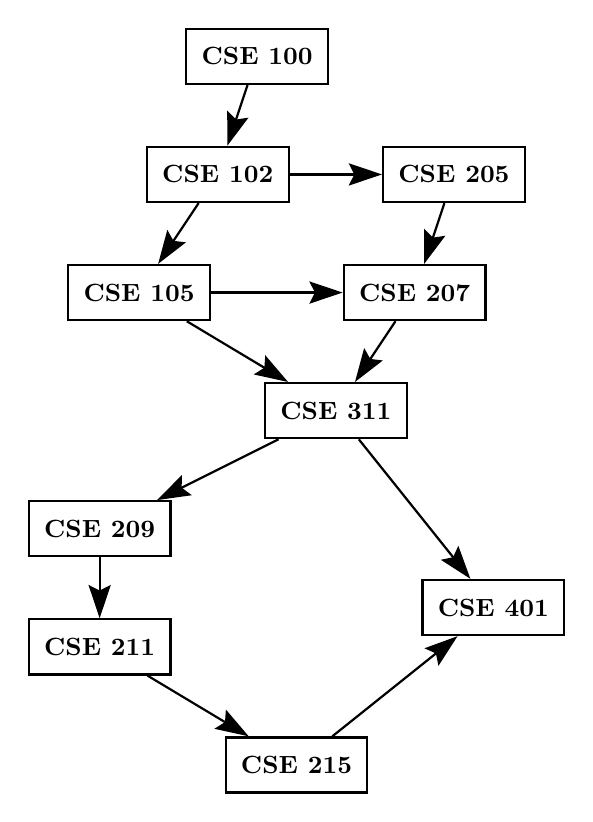
\begin{tikzpicture}[
    every node/.style={rectangle, draw, minimum width=1.8cm,
                       minimum height=0.7cm, font=\small\bfseries},
    every path/.style={->, line width=0.8pt},
  ]
\tikzset{>={Stealth[length=12pt, width=8pt, inset=2pt]}}
  \node (cse100) at (3, 8)    {CSE 100};
  \node (cse102) at (2.5, 6.5){CSE 102};
  \node (cse205) at (5.5, 6.5){CSE 205};
  \node (cse105) at (1.5, 5)  {CSE 105};
  \node (cse207) at (5, 5)    {CSE 207};
  \node (cse311) at (4, 3.5)  {CSE 311};
  \node (cse209) at (1, 2)    {CSE 209};
  \node (cse211) at (1, 0.5)  {CSE 211};
  \node (cse401) at (6, 1)    {CSE 401};
  \node (cse215) at (3.5, -1) {CSE 215};

  \draw (cse100) -> (cse102);
  \draw (cse102) -> (cse205);
  \draw (cse102) -> (cse105);
  \draw (cse205) -> (cse207);
  \draw (cse105) -> (cse207);
  \draw (cse105) -> (cse311);
  \draw (cse207) -> (cse311);
  \draw (cse311) -> (cse401);
  \draw (cse311) -> (cse209);
  \draw (cse209) -> (cse211);
  \draw (cse211) -> (cse215);
  \draw (cse215) -> (cse401);
  \end{tikzpicture}
\end{center}

\end{enumerate}
\newpage

\secdivider{Divide \& Conquer}{Mergesort, Closest Pair, Inversions, Strassen}{cB}{cB}
\markboth{T9 --- Divide \& Conquer}{}
\label{sec:T9}
\section{T9 --- Divide \& Conquer}

\begin{enumerate}
\item Using the recurrence tree method, analyze the runtime complexity of the Mergesort algorithm to sort an array of size $n$. \mk{10}
\yr{CSE 105 | 2023--24}

\item Explain the run-time complexity of the Mergesort algorithm. First, formulate the run-time as a recurrence relation. Then solve the recurrence relation using both: (i) the recurrence tree method, and (ii) the Master theorem (distinguish the case that is applicable in your analysis). \mk{2+5+3=10}
\yr{CSE 105 | 2022--23}

\item Given a sequence of $n$ numbers $a_1, \ldots, a_n$ (all distinct), define an \textit{inversion} as a pair $i < j$ such that $a_i > a_j$. Present an $O(n \log n)$ divide-and-conquer algorithm to count the number of inversions. Define a \textit{modified-inversion} as a pair where $i < j$ and $a_i > 2a_j$. What modifications are needed in the divide-and-conquer algorithm to count the number of modified-inversions? \mk{20}
\yr{CSE 105 | 2021--22}

\item Given $n$ points $(x_1, y_1), (x_2, y_2), \ldots, (x_n, y_n)$ in the plane, give an efficient divide-and-conquer algorithm to find the pair of points that is closest together. Prove the correctness and analyze the running time of your algorithm. \mk{17}
\yr{CSE 105 | 2021--22, 2016--17}

\item Provide a divide-and-conquer algorithm that takes an $n$-digit number $A$ as input and efficiently computes the square of $A$ with a faster asymptotic running time than $O(n^2)$. Analyze the running time. \mk{12}
\yr{CSE 203 | 2021--22}

\item Suppose, in a 2-dimensional co-ordinate system, you are given with $n$
points, say $P_1, P_2, \ldots, P_n$, where the $x$-$y$ co-ordinates of any
point $P_i$ is represented as $(x_i, y_i)$. You have been assigned to find the
closest pair of points using divide and conquer method.
\begin{enumerate}[label=(\roman*)]
  \item Write down the approach that you will follow to split these $n$ points
  into two partitions, say \textit{LEFT} and \textit{RIGHT}, in such a way that
  each partition contains roughly $\dfrac{n}{2}$ points.

  Now suppose, the \textit{LEFT} and \textit{RIGHT} partitions, respectively
  calculate $d_L$ and $d_R$ as the distances between the closest pair of points
  within themselves. Now your task is to check whether there exist a pair of
  points $P_{Li}$ and $P_{Rj}$ such that $P_{Li} \in \textit{LEFT}$ and
  $P_{Rj} \in \textit{RIGHT}$, and the distance between $P_{Li}$ and $P_{Rj}$
  is less than $\min(d_L,\ d_R)$.

  \item Write down the steps to perform this checking so that the minimum number
  of comparisons is ensured and the checking can be performed in $O(n)$ time.
\end{enumerate}
\mk{5+10=15}\yr{CSE 203 | 2020--21}

\item In a sequence of $n$ distinct numbers $a_1, \ldots, a_n$, a \emph{significant inversion} is a pair $i < j$ such that $a_i > 2a_j$. Give an $O(n \log n)$ algorithm to count the number of significant inversions. Write the corresponding pseudocode. \mk{10}
\yr{CSE 203 | 2020--21}

\item Write an algorithm to find a peak element of an $n \times n$ matrix in $O(n)$ time using divide and conquer. A peak element is one whose left, right, top, and bottom neighbors (if available) are all smaller. Define the recurrence relation and derive the runtime. \mk{10+5}
\yr{CSE 203 | 2019--20}

\item Propose the pseudocode of a merge sort algorithm where the array is divided into three equal parts at each step. Derive the asymptotic runtime of this algorithm. Compare it with standard merge sort (two equal parts) and mention cases when one outperforms the other. \mk{10+8+7}
\yr{CSE 203 | 2019--20}

\item Explain how a recursion tree can help with the substitution method of runtime analysis. \mk{5}
\yr{CSE 203 | 2019--20}

\item Write a divide-and-conquer algorithm that finds the maximum and the minimum of an array of $n$ distinct elements. Write the recurrence relation for the running time $T(n)$ and solve it using the Recursion Tree Method. \mk{10}
\yr{CSE 203 | 2018--19}

\item Write the Mergesort algorithm. Simulate it on the array $[6, 1, 7, 2, 8, 3, 9, 4, 10, 5, 11, 17, 4, 5]$. \mk{15}
\yr{CSE 203 | 2017--18}

\item Given a sorted array of distinct integers $A[1 \ldots n]$, give a divide-and-conquer algorithm that runs in $O(\log n)$ time to find whether there is an index $i$ for which $A[i] = i$. Write the pseudocode and prove the runtime. \mk{12}
\yr{CSE 207 | 2014--15}

\item Explain the divide-and-conquer technique. What is the function of the pivot element in the Quicksort algorithm? \mk{3+2=5}
\yr{CSE 203 | 2012--13}

\item Use a recursion tree to determine a good asymptotic upper bound on the recurrence $T(n) = T(n/4) + T(n/2) + n^2$. \mk{10}
\yr{CSE 207 | 2012--13}

\item What is the divide-and-conquer technique? \mk{5}
\yr{CSE 203 | 2011--12}

\item Write the Mergesort algorithm. Analyze the time complexity of the algorithm. \mk{10+5=15}
\yr{CSE 203 | 2011--12}

\item Write the recurrence relation of the Mergesort algorithm. Draw the recursion tree for the recurrence relation of the Mergesort algorithm. \mk{7}
\yr{CSE 203 | 2011--12}

\item In the closest-pair-of-points problem using the divide-and-conquer approach, if $q$ is a point in the left half and $r$ is a point in the right half, and $d(q,r) < \delta$, where $\delta$ is the minimum of distances in each half, then show that each of $q$ and $r$ lies within a distance $\delta$ of the line dividing the two halves. Hence show that $q$ and $r$ are within 11 positions of each other in a list sorted by $y$-coordinate. \mk{15}
\yr{CSE 207 | 2011--12}

\end{enumerate}
\newpage

\secdivider{Greedy Methods}{MST (Kruskal, Prim), Huffman, Activity Selection, Dijkstra}{cC}{cC}
\markboth{T10 --- Greedy Methods}{}
\label{sec:T10}
\section{T10 --- Greedy Methods}

\begin{enumerate}
\item Define the Activity Selection Problem. Prove that the greedy choice of selecting activities based on earliest finish time yields an optimal solution. \mk{5+10=15}
\yr{CSE 105 | 2023--24}
%% ---------------------------------------------------------------------
%% Q: Activity Selection Problem --- definition + greedy proof.
%%    [CSE 105 | 2023--24]
%% ---------------------------------------------------------------------

\item Apply Prim's algorithm to find the minimum spanning tree of the given graph.

\begin{center}

  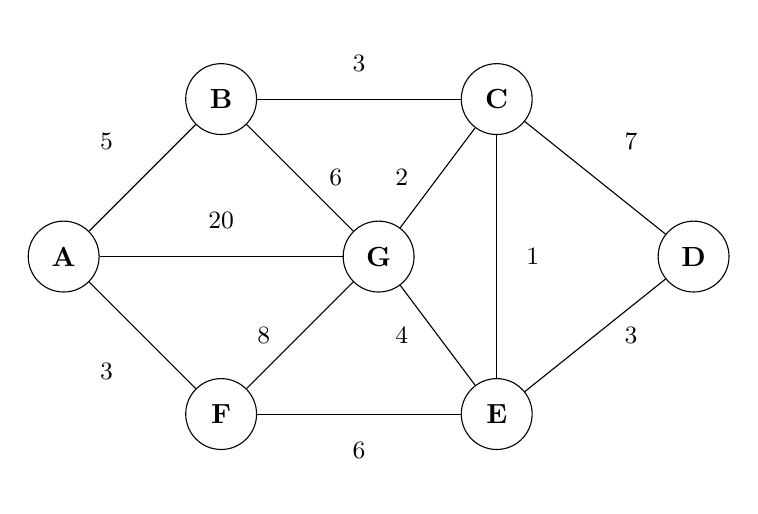
\begin{tikzpicture}[
    every node/.style={circle, draw, minimum size=0.9cm, font=\bfseries},
    edge label/.style={rectangle, draw=none, font=\normalfont\small},
  ]

  \node (A) at (0, 0)    {A};
  \node (B) at (2, 2)    {B};
  \node (C) at (5.5, 2)    {C};
  \node (F) at (2, -2)   {F};
  \node (G) at (4, 0)  {G};
  \node (E) at (5.5, -2) {E};
  \node (D) at (8, 0)    {D};

  \draw (A) -- node[edge label, above left]  {5}  (B);
  \draw (A) -- node[edge label, below left]  {3}  (F);
  \draw (A) -- node[edge label, above]       {20} (G);
  \draw (B) -- node[edge label, above]       {3}  (C);
  \draw (B) -- node[edge label, right]       {6}  (G);
  \draw (C) -- node[edge label, left]       {2}  (G);
  \draw (C) -- node[edge label, above right] {7}  (D);
  \draw (F) -- node[edge label, left]        {8}  (G);
  \draw (F) -- node[edge label, below]       {6}  (E);
  \draw (G) -- node[edge label, left]       {4}  (E);
  \draw (C) -- node[edge label, right]       {1}  (E);
  \draw (D) -- node[edge label, right]       {3}  (E);

  \end{tikzpicture}

\end{center}

Start with node $A$ as the root node. At each step, show the intermediate MST (i.e., the partial tree) and show the estimated cost to connect each non-visited node (i.e., the minimum weight of an edge connecting an unvisited node to any visited nodes).The first step , where only the root node is included in the tree , is done for you . \mk{10}
\yr{CSE 105 | 2023--24}

\begin{center}
  \begin{tikzpicture}[
    every node/.style={circle, draw, minimum size=1.1cm, font=\bfseries},
    label/.style={rectangle, draw=none, font=\normalfont\small},
  ]

  % Root arrow
  \node[draw=none] (root) at (-2, 0) {Root};

  \node (A) at (0, 0)    {A};
  \node (B) at (2, 2)    {B};
  \node (C) at (5.5, 2)    {C};
  \node (F) at (2, -2)   {F};
  \node (G) at (4, 0)  {G};
  \node (E) at (5.5, -2) {E};
  \node (D) at (8, 0)    {D};

  % Root arrow
  \draw[->, >=stealth] (root) -> (A);

  % Distance labels above/below each node
  \node[label, above] at (B.north) {5};
  \node[label, above] at (C.north) {$\infty$};
  \node[label, below] at (F.south) {3};
  \node[label, above] at (G.north) {20};
  \node[label, below] at (E.south) {$\infty$};
  \node[label, above] at (D.north) {$\infty$};

  \end{tikzpicture}
 \end{center}
 

\item Argue in favor of the correctness of Prim's algorithm to find a minimum spanning tree of a graph $G = (V, E)$. Prove any non-trivial graph properties used in the argument. \mk{5+10=15}
\yr{CSE 105 | 2022--23}
%% ---------------------------------------------------------------------
%% Q: Correctness of Prim's algorithm.  [CSE 105 | 2022--23]
%% ---------------------------------------------------------------------

\item  Find the shortest path distance from every node $x$  to node $t$ in the given graph using Dijkstra's Algorithm. Re-draw the diagram for each intermediate step of the algorithm (after relaxation) while annotating each node with the appropriate shortest path distance estimate of that step. \mk{10}
\yr{CSE 105 | 2022--23}

\begin{center}
  
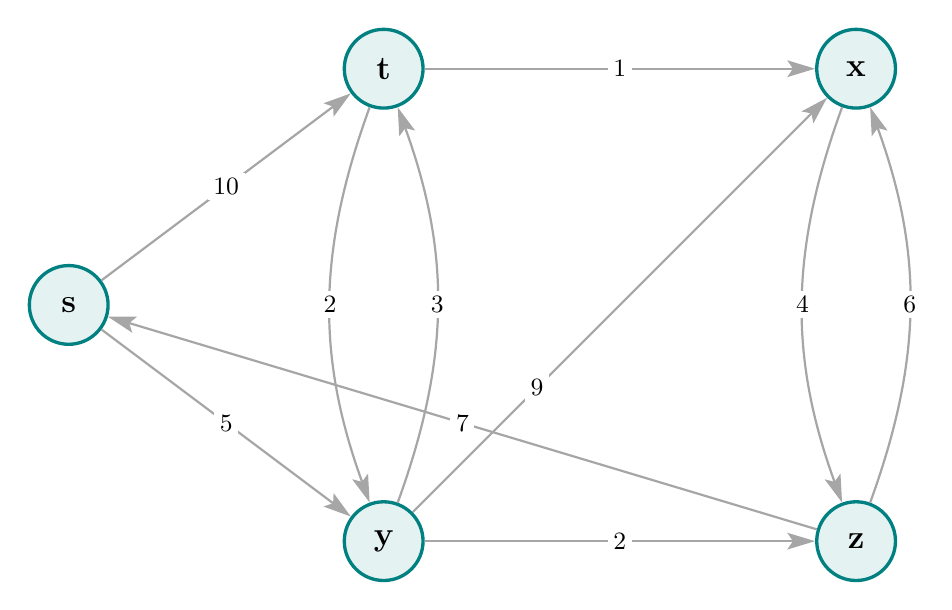
\begin{tikzpicture}[
    % Define professional colors
    node outline/.style={draw=teal, very thick},
    node fill/.style={fill=teal!10},
    % Modern circular node style
    my node/.style={circle, node outline, node fill, minimum size=1cm, font=\bfseries\large, text centered},
    % Clean arrow style
    my edge/.style={->, >={Stealth[length=10pt, width=6pt, inset=2pt]}, thick, draw=gray!70},
    % Standard label style (white background makes it easy to read over lines)
    edge label/.style={fill=white, inner sep=2pt, font=\normalfont\small, midway}
  ]

  % --- Node Definitions ---
  \node[my node] (s) at (0, 0)     {s};
  \node[my node] (t) at (4, 3)     {t};
  \node[my node] (x) at (10, 3)    {x};
  \node[my node] (y) at (4, -3)    {y};
  \node[my node] (z) at (10, -3)   {z};

  % --- Edge Definitions ---
  \begin{scope}[my edge]
    % Straight edges
    \draw (s) -- node[edge label] {10} (t);
    \draw (s) -- node[edge label] {5}  (y);
    \draw (t) -- node[edge label] {1}  (x);
    \draw (y) -- node[edge label, pos=0.3] {9} (x); % pos=0.3 to prevent overlapping in the middle
    \draw (y) -- node[edge label] {2}  (z);

    % Symmetrical pairs of bent edges (y <-> t and x <-> z)
    \draw (t) to[bend right=20] node[edge label] {2} (y);
    \draw (y) to[bend right=20] node[edge label] {3} (t);
    \draw (x) to[bend right=20] node[edge label] {4} (z);
    \draw (z) to[bend right=20] node[edge label] {6} (x);

    % Bent long return edge
    \draw (z) to[bend left=0]  node[edge label] {7} (s);
  \end{scope}

\end{tikzpicture}
\end{center}
%% ---------------------------------------------------------------------
%% Q: Dijkstra from s; find dist to all nodes.
%%    [CSE 105 | 2022--23]   ← Python verified \checkmark{}
%%    Final: s=0, y=5, z=7, t=8, x=9
%% ---------------------------------------------------------------------
%% ---------------------------------------------------------------------
%% Q: Dijkstra from s; find dist to all nodes.
%%    [CSE 105 | 2022--23]
%% ---------------------------------------------------------------------

\item Given a set $U = \{x_1, x_2, \ldots, x_n\}$ of $n$ integers and an integer $k$ ($k < n$), give an optimal greedy algorithm to find a subset $S$ of size $k$ in $U$ such that the summation of the numbers in $S$ is maximum (over all subsets of size $k$ in $U$). Prove the correctness of your algorithm and analyze its running time. \mk{15}
\yr{CSE 105 | 2021--22}
%% ---------------------------------------------------------------------
%% Q: Greedy algorithm to find subset S of size k with max sum.
%%    [CSE 105 | 2021--22]
%% ---------------------------------------------------------------------

\item Consider a set of $n$ intervals where each interval $i$ specifies a start time $s_i$ and a finish time $f_i$ ($s_i < f_i$). Two intervals are compatible if they do not overlap. Give a greedy algorithm to select a compatible subset of maximum possible size. Prove the correctness and analyze the running time. \mk{16}
\yr{CSE 203 | 2021--22}
%% ---------------------------------------------------------------------
%% Q: Greedy interval scheduling --- algorithm, correctness, runtime.
%%    [CSE 203 | 2021--22]
%% ---------------------------------------------------------------------

\item Given a set $S = \{x_1, x_2, \ldots, x_n\}$ of real numbers where $x_1 \leq x_2 \leq \cdots \leq x_n$, write a greedy algorithm to determine the smallest set of unit-length intervals that contain all numbers in $S$. Prove correctness and analyze running time. \mk{15}
\yr{CSE 203 | 2021--22}
%% ---------------------------------------------------------------------
%% Q: Minimum unit-length intervals --- algorithm, correctness, runtime.
%%    [CSE 203 | 2021--22]  (same as [2017--18] --- refer to that answer)
%% ---------------------------------------------------------------------

\item Once upon a time there was a city that had no proper roads. Getting around
the city was particularly difficult after rainstorms because the ground used to
become very muddy, cars got stuck in the mud, and people got their boots dirty.
The mayor of the city decided that some of the streets must be paved, but he did
not want to spend more money than necessary because the city also wanted to build
a swimming pool. The mayor therefore specified two conditions:
\begin{enumerate}[label=(\roman*)]
  \item Enough streets must be paved so that it is possible for everyone to
  travel from their house to anyone else's house only along the paved roads, and
  \item The paving should cost as little as possible.
\end{enumerate}
The following figure shows the layout of the city. The number of paving stones
in between two houses represents the cost of paving that route. Your task is to
apply a greedy based algorithm that you have learned under this course to fulfill
the requirement of the Mayor. Note that the bridge in the figure should not be
considered as a paving stone. In your answer script, you must draw a simple
graph representing the given layout of the muddy city. After that, you have to
show the steps of applying your chosen greedy algorithm to find the connected
subgraph which contains all the houses of the city (considering them as vertices
of your drawn graph) and a subset of roads (considering them as edges) in a way
that the total number of paving stones required is the minimum. You have to
ensure that your connected subgraph does not contain any cycle, and you need to
mention the algorithm that you are adopting to find your desired solution.
\mk{15}
\yr{CSE 203 | 2020--21}

\begin{center}
  
\includegraphics[width=0.75\textwidth,keepaspectratio]{/193.png}
\end{center}

%% ---------------------------------------------------------------------
%% Q: The Muddy City (Minimum Spanning Tree) - Final Corrected Version
%% ---------------------------------------------------------------------

\item Prove that an optimal solution is always guaranteed if we design an activity-selection greedy algorithm by always choosing the activity with the earliest finish time from the remaining compatible activities. \mk{10}
\yr{CSE 203 | 2020--21}
%% ---------------------------------------------------------------------
%% Q: Prove activity-selection greedy (earliest finish) is optimal.
%%    [CSE 203 | 2020--21]
%% ---------------------------------------------------------------------

\item Analyze the runtime complexity of MST-Prim's algorithm (as given using a Binary Min-Heap to maintain a minimum priority queue), mentioning the individual runtime of each significant operation. How is this running time improved if a Fibonacci Heap is used instead? \mk{10}
\yr{CSE 203 | 2020--21}
%% ---------------------------------------------------------------------
%% Q: Prim's runtime with binary min-heap; improvement with Fibonacci heap.
%%    [CSE 203 | 2020--21]
%% ---------------------------------------------------------------------

\item Write an algorithm to calculate the maximum profit earned by executing tasks within specified deadlines. A task takes one unit of time to execute and cannot execute beyond its deadline; only one task executes at a time. Apply the algorithm to the following data:
\begin{center}
\begin{tabular}{lcccccccccc}
\toprule
Task & T1 & T2 & T3 & T4 & T5 & T6 & T7 & T8 & T9 & T10 \\
Deadline & 7 & 3 & 2 & 6 & 8 & 5 & 6 & 3 & 2 & 4 \\
Profit & 9 & 14 & 5 & 10 & 3 & 15 & 5 & 7 & 8 & 6 \\
\bottomrule
\end{tabular}
\end{center}
\mk{10+10}
\yr{CSE 203 | 2019--20}
%% ---------------------------------------------------------------------
%% Q: Job scheduling T1-T10 --- max profit.
%%    [CSE 203 | 2019--20]   ← Python verified \checkmark{}  Total = 72
%% ---------------------------------------------------------------------
%% ---------------------------------------------------------------------
%% Q: Job scheduling T1-T10 --- max profit.
%%    [CSE 203 | 2019--20]   ← Python verified \checkmark{}  Total = 72
%% ---------------------------------------------------------------------

\item Show that the fractional knapsack problem has the optimal substructure property. Also show that the 0-1 knapsack problem has the overlapping subproblems property. \mk{10}
\yr{CSE 203 | 2018--19}
%% ---------------------------------------------------------------------
%% Q: Fractional knapsack --- optimal substructure; 0-1 knapsack ---
%%    overlapping subproblems.  [CSE 203 | 2018--19]
%% ---------------------------------------------------------------------

\item Prove that an optimal minimum spanning tree is composed of optimal minimum spanning subtrees. Draw a minimum spanning tree containing the edges with weights $x$ and $z$. \mk{15}
\yr{CSE 207 | 2018--19}

\begin{center}
  
  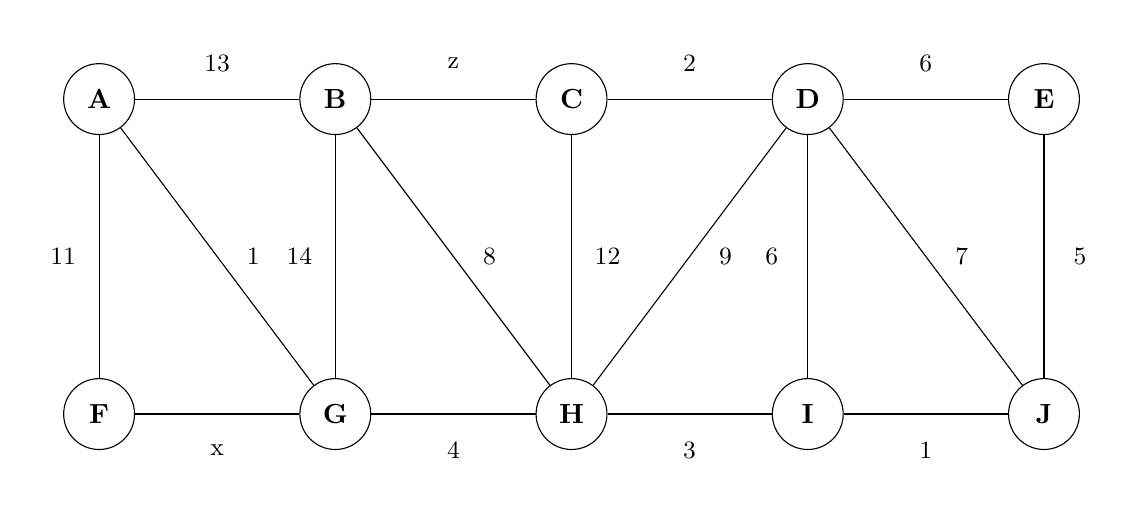
\begin{tikzpicture}[
    every node/.style={circle, draw, minimum size=0.9cm, font=\bfseries},
    edge label/.style={rectangle, draw=none, font=\normalfont\small},
  ]

  % Top row
  \node (A) at (0, 4)  {A};
  \node (B) at (3, 4)  {B};
  \node (C) at (6, 4)  {C};
  \node (D) at (9, 4)  {D};
  \node (E) at (12, 4)  {E};

  % Bottom row
  \node (F) at (0, 0)  {F};
  \node (G) at (3, 0)  {G};
  \node (H) at (6, 0)  {H};
  \node (I) at (9, 0)  {I};
  \node (J) at (12, 0)  {J};

  % Top row edges
  \draw (A) -- node[edge label, above] {13} (B);
  \draw (B) -- node[edge label, above] {z}  (C);
  \draw (C) -- node[edge label, above] {2}  (D);
  \draw (D) -- node[edge label, above] {6}  (E);

  % Bottom row edges
  \draw (F) -- node[edge label, below] {x}  (G);
  \draw (G) -- node[edge label, below] {4}  (H);
  \draw (H) -- node[edge label, below] {3}  (I);
  \draw (I) -- node[edge label, below] {1}  (J);

  % Vertical & diagonal edges
  \draw (A) -- node[edge label, left]        {11} (F);
  \draw (E) -- node[edge label, right]       {5}  (J);
  \draw (A) -- node[edge label, right]       {1}  (G);
  \draw (B) -- node[edge label, left]        {14} (G);
  \draw (B) -- node[edge label, right]       {8}  (H);
  \draw (C) -- node[edge label, right]       {12} (H);
  \draw (D) -- node[edge label, right]       {9}  (H);
  \draw (D) -- node[edge label, left]        {6}  (I);
  \draw (D) -- node[edge label, right]       {7}  (J);

  \end{tikzpicture}

\end{center}

%% ---------------------------------------------------------------------
%% Q: MST has optimal substructure; draw MST containing edges x and z.
%%    [CSE 207 | 2018--19] 
%% ---------------------------------------------------------------------

\item Write down an algorithm for job sequencing with deadlines. Solve the problem instance with profit and deadline values $(p_i, d_i)$ as follows: $(7,5),(6,5),(5,2),(4,7),(3,7),\\(3,7),(3,6),(2,7),(2,1),(2,5),(2,3),(2,1),(1,1)$. \mk{10+10}
\yr{CSE 203 | 2017--18}

%% ---------------------------------------------------------------------
%% Q: Job scheduling with deadlines (Algorithm + Execution)
%%    [CSE 203 | 2017--18]
%% ---------------------------------------------------------------------

\item Give an optimal greedy algorithm for solving the fractional knapsack problem. Prove that your algorithm is optimal. \mk{13}
\yr{CSE 203 | 2017--18}
%% ---------------------------------------------------------------------
%% Q: Fractional knapsack --- algorithm + optimality proof.
%%    [CSE 203 | 2017--18]
%% ---------------------------------------------------------------------

\item Given a set $S = \{x_1, x_2, \ldots, x_n\}$ of real numbers where
$x_1 \leq x_2 \leq \ldots \leq x_n$, write a greedy algorithm to determine
the smallest set of unit-length intervals that contain all the numbers in $S$.
For example, an interval $[1.5,\ 2.5]$ is a unit length interval (since
$2.5 - 1.5 = 1$), and it contains all the real numbers from 1.5 to 2.5
(including 1.5 and 2.5). You have to find the smallest set of such unit length
intervals which contains all the real numbers in $S$. Prove the correctness of
your algorithm, and analyze the running time. \mk{15}\yr{CSE 203 | 2017--18}

%% ---------------------------------------------------------------------
%% Q: Minimum unit-length intervals --- algorithm + correctness.
%%    [CSE 203 | 2017--18]
%% ---------------------------------------------------------------------

\item Write down an algorithm for constructing a minimum spanning tree. Construct the MST for the graph defined by the edges: $ra(7), rx(2), ax(1), xy(5), ya(3), xc(6), cb(4),\\ bx(2), yb(2)$, where the weight of each edge is given in parentheses. \mk{10+10}
\yr{CSE 203 | 2017--18}

%% ---------------------------------------------------------------------
%% Q: Kruskal's MST for ra(7),rx(2),ax(1),xy(5),ya(3),xc(6),
%%    cb(4),bx(2),yb(2).  [CSE 203 | 2017--18] 
%% ---------------------------------------------------------------------

\item What is a spanning tree of a graph? Write Kruskal's algorithm for finding a minimum spanning tree of an edge-weighted graph. Analyze the time complexity of the algorithm by suggesting appropriate data structures. \mk{3+5+7}
\yr{CSE 207 | 2017--18}
%% ---------------------------------------------------------------------
%% Q: Spanning tree definition; Kruskal + complexity.
%%    [CSE 207 | 2017--18]
%% ---------------------------------------------------------------------

\item Find a minimum spanning tree using Prim's algorithm, showing every step. \mk{10}
\yr{CSE 207 | 2017--18}

\begin{center}
  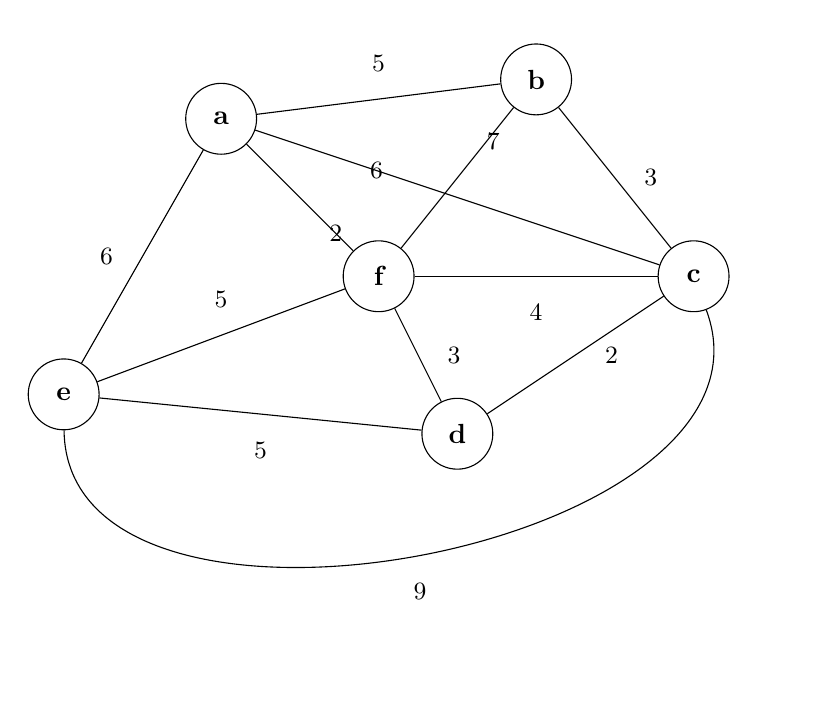
\begin{tikzpicture}[
    every node/.style={circle, draw, minimum size=0.9cm, font=\bfseries},
    edge label/.style={rectangle, draw=none, font=\normalfont\small},
  ]

  \node (a) at (2, 4)   {a};
  \node (b) at (6, 4.5) {b};
  \node (c) at (8, 2) {c};
  \node (d) at (5, 0)   {d};
  \node (e) at (0, 0.5) {e};
  \node (f) at (4, 2)   {f};

  \draw (a) -- node[edge label, above]       {5} (b);
  \draw (a) -- node[edge label, below right] {2} (f);
  \draw (a) -- node[edge label, left]        {6} (e);
  \draw (a) -- node[edge label, pos=0.3]       {6} (c);
  \draw (b) -- node[edge label, right]       {3} (c);
  \draw (b) -- node[edge label, above right] {7} (f);
  \draw (f) -- node[edge label, below]       {4} (c);
  \draw (f) -- node[edge label, right]       {3} (d);
  \draw (c) -- node[edge label, right]       {2} (d);
  \draw (e) -- node[edge label, above]       {5} (f);
  \draw (e) -- node[edge label, below]       {5} (d);
  \draw (c) to[bend left=100] node[edge label, below] {9} (e);

  \end{tikzpicture}

\end{center}

%% ---------------------------------------------------------------------
%% Q: Find a minimum spanning tree using Prim's algorithm
%%    [CSE 207 | 2017--18] 
%% ---------------------------------------------------------------------

%% ══════════════════════════════════════════════════════════════════════
%% ANSWER SNIPPETS --- MST Proofs, Huffman, Greedy Proofs (Batch 3)
%% ALL simulation results verified by Python before writing LaTeX.
%% ══════════════════════════════════════════════════════════════════════

\item Let $G$ be a weighted connected graph and let $V_1, V_2$ be a partition of its vertices into two disjoint non-empty sets. Let $e$ be an edge in $G$ with minimum weight among those with one endpoint in $V_1$ and the other in $V_2$. Show that there is a minimum spanning tree $T$ of $G$ containing $e$. \mk{10}
\yr{CSE 207 | 2017--18}
%% ---------------------------------------------------------------------
%% Q: Show minimum-weight crossing edge e is in some MST.
%%    [CSE 207 | 2017--18]
%% ---------------------------------------------------------------------

\item Huffman's algorithm is used to obtain an encoding of alphabet $\{a, b, c\}$ with frequencies $f_a$, $f_b$, and $f_c$. In each of the following cases, either give an example of frequencies that would yield the specified code, or explain why the code cannot possibly be obtained:
\begin{enumerate}
  \item Code: $\{0, 10, 11\}$
  \item Code: $\{0, 1, 00\}$
  \item Code: $\{10, 01, 00\}$
\end{enumerate}
Then construct Huffman codes for the characters with the following frequencies: A:24, B:12, C:10, D:8, E:9, F:37, using the greedy algorithm. \mk{6+9}
\yr{CSE 203 | 2016--17}
%% ---------------------------------------------------------------------
%% Q: Huffman coding for {a,b,c}; code validity; build for A-F.
%%    [CSE 203 | 2016--17]   ← Python verified \checkmark{}
%% ---------------------------------------------------------------------

\item Suppose you are given $n$ white and $n$ black dots, lying on a line. The dots
are equally spaced but they may appear in any order of black and white (black and
white may be interleaved). Design a greedy algorithm to connect each black dot with
a (different) white dot so that the total length of wires used to connect the dots
is minimal. The length of wire used to connect two dots is equal to their distance
along the line. Prove that your algorithm is optimal.

\begin{center}
\begin{tabular}{|c|c|c|c|c|c|c|c|}
\hline
$\bullet$ & $\bullet$ & $\circ$ & $\bullet$ & $\circ$ & $\circ$ & $\circ$ & $\bullet$ \\
\hline
1 & 2 & 3 & 4 & 5 & 6 & 7 & 8 \\
\hline
\end{tabular}
\end{center}

For example, an optimal solution to solve the above example is $(1,3)$, $(2,5)$,
$(4,6)$, $(7,8)$ with total wire length $= 2+3+2+1 = 8$. \mk{15}\yr{CSE 203 | 2016--17}

%% ---------------------------------------------------------------------
%% Q: Black-white dot matching --- greedy + optimality proof.
%%    [CSE 203 | 2016--17]   ← Python verified \checkmark{}
%%    Blacks: 1,2,4,8 Whites: 3,5,6,7 $\rightarrow$ pairs (1,3),(2,5),(4,6),(8,7) total=8
%% ---------------------------------------------------------------------

\item Write Prim's algorithm that computes a minimum spanning tree of a graph. Analyze its time complexity. \mk{15}
\yr{CSE 207 | 2016--17}
%% ---------------------------------------------------------------------
%% Q: Prim's algorithm --- write + complexity.  [CSE 207 | 2016--17]
%% ---------------------------------------------------------------------

\item Write the correctness proof of Kruskal's algorithm for finding a minimum spanning tree. \mk{10}
\yr{CSE 207 | 2016--17}
%% ---------------------------------------------------------------------
%% Q: Correctness proof of Kruskal's algorithm.  [CSE 207 | 2016--17]
%% ---------------------------------------------------------------------

\item Compare the key properties of problems that can be solved with greedy method, divide-and-conquer method, and dynamic programming method. \mk{10}
\yr{CSE 207 | 2016--17}
%% ---------------------------------------------------------------------
%% Q: Compare greedy / divide-and-conquer / DP.  [CSE 207 | 2016--17]
%% ---------------------------------------------------------------------

\item There is a network of roads $G = (V, E)$ connecting a set of cities $V$.
Each road in $E$ has an associated length $l_e$. There is a proposal to add one
new road to this network, and there is a list $E'$ of pairs of cities between
which the new road can be built. Each such potential road $e' \in E'$ has an
associated length. As a designer for the public works department you are asked
to determine the road $e' \in E'$ whose addition to existing network $G$ would
result in the maximum decrease in the driving distance between two fixed cities
$s$ and $t$ in the network. Give an algorithm for solving this problem. Your
algorithm should run in $O((V + E + E') \log V)$ time. \mk{15}\yr{CSE 207 | 2015--16}

%% ---------------------------------------------------------------------
%% Q: New road to maximally decrease s-t distance.
%%    [CSE 207 | 2015--16]   O((V+E+E') log V)
%% ---------------------------------------------------------------------

\item Find a minimum spanning tree by running (i) Kruskal's algorithm and (ii) Prim's algorithm. Show the order of edges selected in each case (use alphabetical ordering when there is a tie). \mk{15}
\yr{CSE 207 | 2015--16}

\begin{center}

  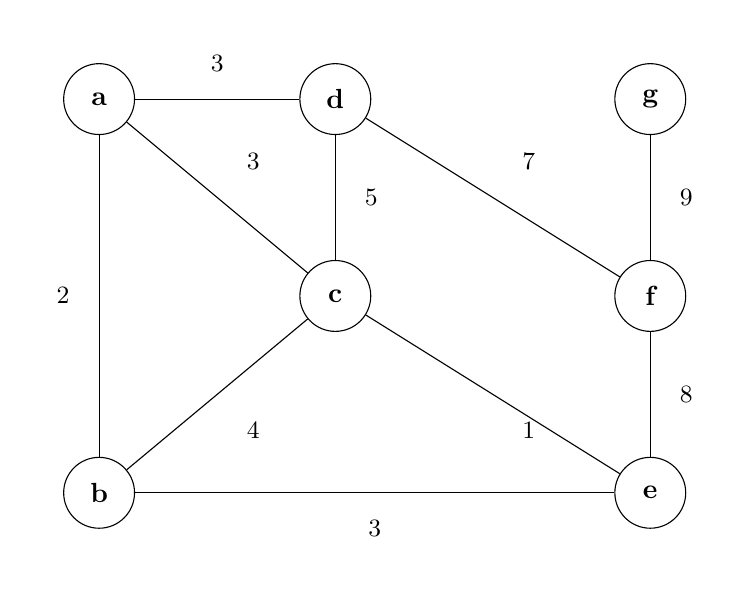
\begin{tikzpicture}[
    every node/.style={circle, draw, minimum size=0.9cm, font=\bfseries},
    edge label/.style={rectangle, draw=none,  font=\normalfont\small},
  ]

  \node (a) at (0, 2)   {a};
  \node (d) at (3, 2)   {d};
  \node (g) at (7, 2)   {g};
  \node (b) at (0, -3)   {b};
  \node (c) at (3, -0.5) {c};
  \node (f) at (7, -0.5) {f};
  \node (e) at (7, -3)   {e};

  \draw (a) -- node[edge label, above]       {3} (d);
  \draw (a) -- node[edge label, left]        {2} (b);
  \draw (a) -- node[edge label, above right] {3} (c);
  \draw (d) -- node[edge label, right]       {5} (c);
  \draw (d) -- node[edge label, above right] {7} (f);
  \draw (g) -- node[edge label, right]       {9} (f);
  \draw (b) -- node[edge label, below right] {4} (c);
  \draw (b) -- node[edge label, below]       {3} (e);
  \draw (c) -- node[edge label, below right] {1} (e);
  \draw (f) -- node[edge label, right]       {8} (e);

  \end{tikzpicture}
\end{center}

%% ---------------------------------------------------------------------
%% Q: Kruskal + Prim on a-g graph with intermediate steps.
%%    [CSE 207 | 2015--16]
%% ---------------------------------------------------------------------

\item Under a Huffman encoding of $n$ symbols with frequencies $f_1, f_2, \ldots, f_n$, what is the longest a codeword could possibly be? Give an example set of frequencies that would produce this case. Then construct Huffman codes for the following frequencies: A:45, B:13, C:12, D:16, E:5, F:9, using the greedy algorithm. \mk{7+8=15}
\yr{CSE 207 | 2015--16}

%% ---------------------------------------------------------------------
%% Q: Huffman --- longest codeword; example; build for A:45,B:13,
%%    C:12,D:16,E:5,F:9.  [CSE 207 | 2015--16]   ← Python verified \checkmark{}
%% ---------------------------------------------------------------------

\item Let $G = (V, E)$ be a connected undirected graph with weight function $w$ on $E$. Let $A \subseteq E$ be included in some MST for $G$, let $(S, V-S)$ be any cut that respects $A$, and let $(u, v)$ be a light edge crossing $(S, V-S)$. Prove that $(u, v)$ is safe for $A$. \mk{10}
\yr{CSE 207 | 2014--15}

%% ---------------------------------------------------------------------
%% Q: Light edge (u,v) safe for A --- proof.  [CSE 207 | 2014--15]
%% ---------------------------------------------------------------------

\item Find the light and respectful crossing edges for each step of Kruskal's method for building the MST. \mk{12}
\yr{CSE 207 | 2014--15}

\begin{center}
  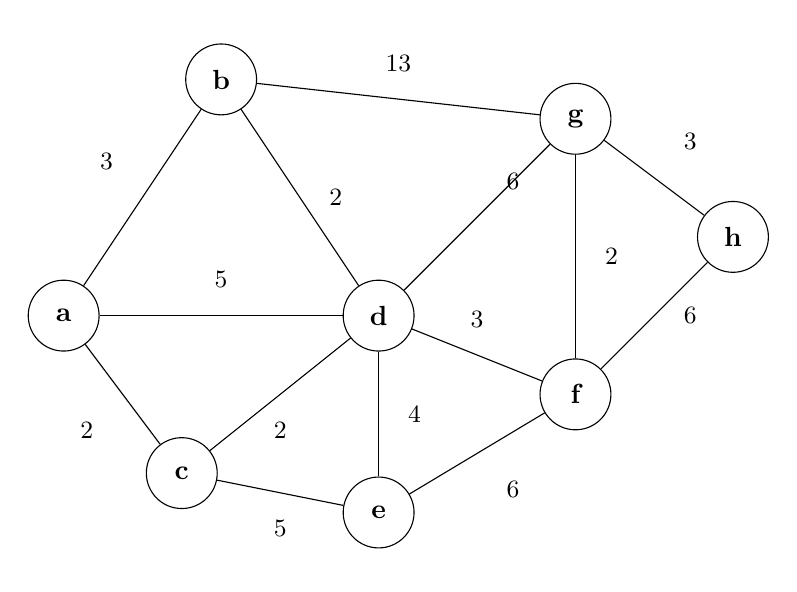
\begin{tikzpicture}[
    every node/.style={circle, draw, minimum size=0.9cm, font=\bfseries},
    edge label/.style={rectangle, draw=none, font=\normalfont\small},
  ]

  \node (a) at (0,   0)    {a};
  \node (b) at (2,   3)    {b};
  \node (c) at (1.5, -2)   {c};
  \node (d) at (4,   0)    {d};
  \node (e) at (4,  -2.5)  {e};
  \node (f) at (6.5, -1)   {f};
  \node (g) at (6.5,  2.5) {g};
  \node (h) at (8.5,  1)   {h};

  \draw (a) -- node[edge label, above left]  {3}  (b);
  \draw (a) -- node[edge label, above]       {5}  (d);
  \draw (a) -- node[edge label, below left]  {2}  (c);
  \draw (b) -- node[edge label, right]       {2}  (d);
  \draw (b) -- node[edge label, above]       {13} (g);
  \draw (c) -- node[edge label, below] {2}  (d);
  \draw (c) -- node[edge label, below]       {5}  (e);
  \draw (d) -- node[edge label, above right] {6}  (g);
  \draw (d) -- node[edge label, above]       {3}  (f);
  \draw (d) -- node[edge label, right]       {4}  (e);
  \draw (e) -- node[edge label, below right] {6}  (f);
  \draw (g) -- node[edge label, right]       {2}  (f);
  \draw (g) -- node[edge label, above right] {3}  (h);
  \draw (h) -- node[edge label, right]       {6}  (f);

  \end{tikzpicture}

\end{center}

\item What is the cost of finding and joining (union) of sets in Kruskal's method? \mk{8}
\yr{CSE 207 | 2014--15}
%% ---------------------------------------------------------------------
%% Q: Kruskal Union-Find cost.  [CSE 207 | 2014--15]
%% ---------------------------------------------------------------------

\item For the graph below, show the value of $u$, $v.key$, $Q$ for the following algorithm (show each step):  \mk{10}
\yr{CSE 207 | 2014--15}

\begin{algorithm}[H]
\caption{\textsc{MST}($G,\, w,\, r$)}
\begin{algorithmic}[1]
\State $Q \gets V[G]$
\For{each $u \in Q$}
    \State $u.key \gets \infty$
\EndFor
\State $r.key \gets 0$;\quad $p[r] \gets \textbf{nil}$
\While{$Q \neq \emptyset$}
    \State $u \gets \textsc{Extract-Min}(Q)$
    \For{each $v \in Adj[u]$}
        \If{$v \in Q$ \textbf{and} $w(u,v) < v.key$}
            \State $p[v] \gets u$
            \State $v.key \gets w(u,v)$
        \EndIf
    \EndFor
\EndWhile
\end{algorithmic}
\end{algorithm}

\begin{center}
  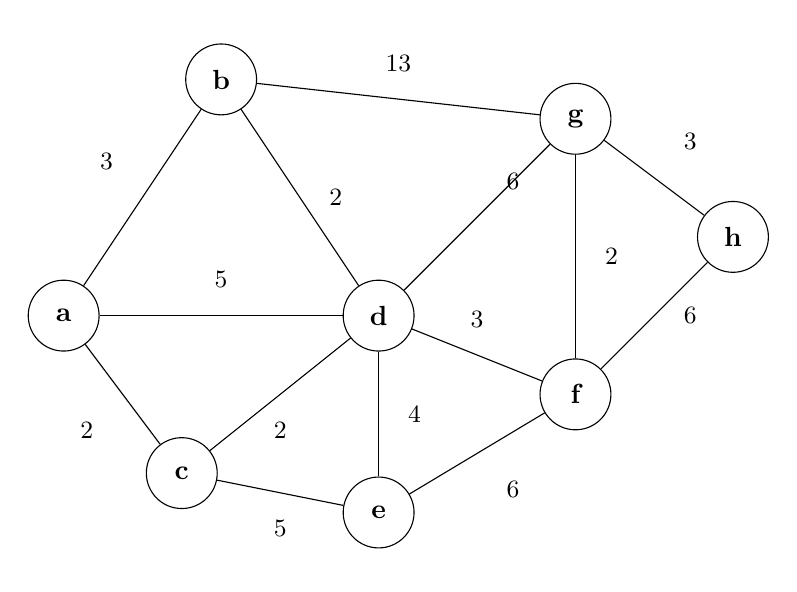
\begin{tikzpicture}[
    every node/.style={circle, draw, minimum size=0.9cm, font=\bfseries},
    edge label/.style={rectangle, draw=none, font=\normalfont\small},
  ]

  \node (a) at (0,   0)    {a};
  \node (b) at (2,   3)    {b};
  \node (c) at (1.5, -2)   {c};
  \node (d) at (4,   0)    {d};
  \node (e) at (4,  -2.5)  {e};
  \node (f) at (6.5, -1)   {f};
  \node (g) at (6.5,  2.5) {g};
  \node (h) at (8.5,  1)   {h};

  \draw (a) -- node[edge label, above left]  {3}  (b);
  \draw (a) -- node[edge label, above]       {5}  (d);
  \draw (a) -- node[edge label, below left]  {2}  (c);
  \draw (b) -- node[edge label, right]       {2}  (d);
  \draw (b) -- node[edge label, above]       {13} (g);
  \draw (c) -- node[edge label, below] {2}  (d);
  \draw (c) -- node[edge label, below]       {5}  (e);
  \draw (d) -- node[edge label, above right] {6}  (g);
  \draw (d) -- node[edge label, above]       {3}  (f);
  \draw (d) -- node[edge label, right]       {4}  (e);
  \draw (e) -- node[edge label, below right] {6}  (f);
  \draw (g) -- node[edge label, right]       {2}  (f);
  \draw (g) -- node[edge label, above right] {3}  (h);
  \draw (h) -- node[edge label, right]       {6}  (f);

  \end{tikzpicture}

\end{center}

\item  \textit{GreedyCell}, a mobile phone operator, wants to place cell towers 
(base stations) along a long straight country road, to provide network coverage to $n$ 
houses sparsely scattered along the road. The distance of these houses from the start 
of the road are, in miles and in increasing order, $d_1, d_2, \ldots, d_n$. Each cell 
tower has coverage of $R$ miles, i.e., if a house is within $R$ miles of a tower, it 
would get service from that tower. Now give an efficient algorithm for finding a 
placement of cell towers that uses as few cell towers as possible to provide coverage 
to all the $n$ houses.\mk{12}
\yr{CSE 207 | 2014--15}
%% ---------------------------------------------------------------------
%% Q: GreedyCell tower placement.  [CSE 207 | 2014--15]
%% ---------------------------------------------------------------------

\item Find a minimum spanning tree using both Kruskal's algorithm and Prim's algorithm (starting from $A$) for the graph with edges: $AB(5), BC(2), AC(4), AD(6), CD(3),\\ DB(1), DE(6), EB(3), EF(3), FB(4)$. \mk{15}
\yr{CSE 207 | 2013--14}

\item Given a set of jobs with start and finish times, write down an algorithm so that the maximum number of jobs can be processed. Show counterexamples for some natural greedy approaches that will not find optimal solutions. \mk{10}
\yr{CSE 207 | 2013--14}
%% ---------------------------------------------------------------------
%% Q: Activity selection --- counterexamples for wrong greedy strategies.
%%    [CSE 207 | 2013--14]
%% ---------------------------------------------------------------------

\item Given the message \texttt{`abaacbdbebfbedcect'}, construct a dynamic Huffman tree showing how the tree is updated after sending each symbol and the code of each symbol. \mk{15}
\yr{CSE 207 | 2013--14}

\item Suppose you are given $n$ tasks with start times $S[1 \ldots n]$ and finish times $F[1 \ldots n]$. Schedule as many tasks as possible so that no two overlap. (i) Describe a greedy algorithm that finds the maximum number of non-overlapping tasks. (ii) Prove the correctness of your greedy algorithm. \mk{15}
\yr{CSE 207 | 2012--13}

\item  If Prim's algorithm is applied on a given graph, which will be the fifth edge added to the spanning tree? Start from vertex $a$. \mk{10}
\yr{CSE 207 | 2012--13}

\begin{center}

  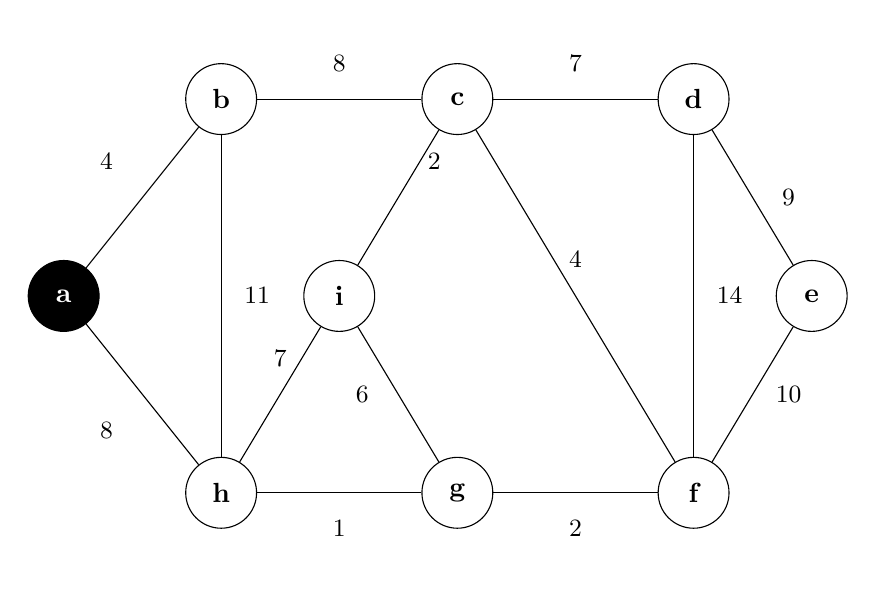
\begin{tikzpicture}[
    every node/.style={circle, draw, minimum size=0.9cm, font=\bfseries},
    edge label/.style={rectangle, draw=none,  font=\normalfont\small},
  ]

  % Nodes (a is filled black)
  \node[fill=black, text=white] (a) at (0, 0)     {a};
  \node (b) at (2,  2.5)  {b};
  \node (c) at (5,  2.5)  {c};
  \node (d) at (8,  2.5)  {d};
  \node (e) at (9.5, 0)   {e};
  \node (f) at (8, -2.5)  {f};
  \node (g) at (5, -2.5)  {g};
  \node (h) at (2, -2.5)  {h};
  \node (i) at (3.5, 0)   {i};

  % Edges
  \draw (a) -- node[edge label, above left]  {4}  (b);
  \draw (a) -- node[edge label, below left]  {8}  (h);
  \draw (b) -- node[edge label, right]       {11} (h);
  \draw (b) -- node[edge label, above]       {8}  (c);
  \draw (c) -- node[edge label, above]       {7}  (d);
  \draw (c) -- node[edge label, above right] {2}  (i);
  \draw (d) -- node[edge label, right]       {9}  (e);
  \draw (d) -- node[edge label, right]       {14} (f);
  \draw (e) -- node[edge label, right]       {10} (f);
  \draw (h) -- node[edge label, above]       {7}  (i);
  \draw (h) -- node[edge label, below]       {1}  (g);
  \draw (i) -- node[edge label, left]        {6}  (g);
  \draw (c) -- node[edge label, above]       {4}  (f);
  \draw (g) -- node[edge label, below]       {2}  (f);

  \end{tikzpicture}

\end{center}

%% ================= GLOBAL DEFINITIONS FOR NEW GRAPH =================
%% TikZ Styles
\tikzset{
  stepnode/.style={circle, draw=black!70, thick, minimum size=0.7cm, font=\bfseries, fill=white},
  visited/.style={fill=blue!15, draw=blue, thick},
  mstedge/.style={very thick, blue},
  highlightedge/.style={very thick, red}, % For the 5th edge
  edgelbl/.style={draw=none, fill=white, font=\small\bfseries, text=black, inner sep=1pt},
  baseedge/.style={-, color=black!60, line width=0.8pt},
  baselbl/.style={draw=none, fill=white, font=\scriptsize, inner sep=1pt, text=black},
  grayedge/.style={-, color=black!15, line width=0.8pt},
  graylbl/.style={draw=none, fill=white, font=\scriptsize, inner sep=1pt, text=black!30},
  lbl/.style={draw=none, fill=none, font=\small\bfseries\color{red!80!black}, inner sep=2pt}
}

%% Graph Edges (Global Definitions using \gdef to prevent scoping errors)
\gdef\drawNewBaseEdges{
  \draw[baseedge] (a) -- node[baselbl, above left]  {4}  (b);
  \draw[baseedge] (a) -- node[baselbl, below left]  {8}  (h);
  \draw[baseedge] (b) -- node[baselbl, right]       {11} (h);
  \draw[baseedge] (b) -- node[baselbl, above]       {8}  (c);
  \draw[baseedge] (c) -- node[baselbl, above]       {7}  (d);
  \draw[baseedge] (c) -- node[baselbl, above right] {2}  (i);
  \draw[baseedge] (d) -- node[baselbl, right]       {9}  (e);
  \draw[baseedge] (d) -- node[baselbl, right]       {14} (f);
  \draw[baseedge] (e) -- node[baselbl, right]       {10} (f);
  \draw[baseedge] (h) -- node[baselbl, above]       {7}  (i);
  \draw[baseedge] (h) -- node[baselbl, below]       {1}  (g);
  \draw[baseedge] (i) -- node[baselbl, left]        {6}  (g);
  \draw[baseedge] (c) -- node[baselbl, above]       {4}  (f);
  \draw[baseedge] (g) -- node[baselbl, below]       {2}  (f);
}

\gdef\drawNewFaintEdges{
  \draw[grayedge] (a) -- node[graylbl, above left]  {4}  (b);
  \draw[grayedge] (a) -- node[graylbl, below left]  {8}  (h);
  \draw[grayedge] (b) -- node[graylbl, right]       {11} (h);
  \draw[grayedge] (b) -- node[graylbl, above]       {8}  (c);
  \draw[grayedge] (c) -- node[graylbl, above]       {7}  (d);
  \draw[grayedge] (c) -- node[graylbl, above right] {2}  (i);
  \draw[grayedge] (d) -- node[graylbl, right]       {9}  (e);
  \draw[grayedge] (d) -- node[graylbl, right]       {14} (f);
  \draw[grayedge] (e) -- node[graylbl, right]       {10} (f);
  \draw[grayedge] (h) -- node[graylbl, above]       {7}  (i);
  \draw[grayedge] (h) -- node[graylbl, below]       {1}  (g);
  \draw[grayedge] (i) -- node[graylbl, left]        {6}  (g);
  \draw[grayedge] (c) -- node[graylbl, above]       {4}  (f);
  \draw[grayedge] (g) -- node[graylbl, below]       {2}  (f);
}
%% ======================================================

\item ``Search spaces for natural combinatorial problems tend to grow exponentially with the size of the input'' --- explain and justify with necessary examples. \mk{15}
\yr{CSE 207 | 2011--12}
%% ---------------------------------------------------------------------
%% Q: Exponential search spaces in combinatorics.
%%    [CSE 207 | 2011--12]
%% ---------------------------------------------------------------------

%%---------------------------------------------------------------------
\item Explain why one can solve the fractional knapsack problem by a greedy
strategy, but one cannot solve the 0-1 knapsack problem by such a strategy.
\mk{10}
\yr{CSE 207 | 2011--12}

\item Prove that the greedy method stays ahead in the interval scheduling problem, and hence show that the greedy method returns an optimal set of jobs. \mk{15}
\yr{CSE 207 | 2011--12}
%% ---------------------------------------------------------------------
%% Q: Greedy stays ahead --- interval scheduling proof.
%%    [CSE 207 | 2011--12]
%% ---------------------------------------------------------------------

\item Prove that if we use a greedy algorithm for the interval partitioning problem, every interval will be assigned a label, and no two overlapping intervals will receive the same label. \mk{15}
\yr{CSE 207 | 2011--12}
%% ---------------------------------------------------------------------
%% Q: Interval partitioning --- greedy assigns every interval, no two
%%    overlapping intervals share a label.  [CSE 207 | 2011--12]
%% ---------------------------------------------------------------------

\item Explain how Dijkstra's algorithm can be implemented using a priority queue. Find the running time for this algorithm. \mk{15}
\yr{CSE 207 | 2011--12}
%% ---------------------------------------------------------------------
%% Q: Dijkstra with priority queue; running time.
%%    [CSE 207 | 2011--12]
%% ---------------------------------------------------------------------

\item State and prove the ``cut property'' and the ``cycle property''. Explain with necessary examples how these properties are useful in solving the minimum spanning tree problem. \mk{15}
\yr{CSE 207 | 2011--12}
%% ---------------------------------------------------------------------
%% Q: Cut property and cycle property; MST application.
%%    [CSE 207 | 2011--12]
%% ---------------------------------------------------------------------

\item Describe, with necessary elaboration on the required operations and data structure, how the union-find data structure can be used for Kruskal's algorithm. \mk{15}
\yr{CSE 207 | 2011--12}
%% ---------------------------------------------------------------------
%% Q: Union-Find for Kruskal's algorithm.  [CSE 207 | 2011--12]
%% ---------------------------------------------------------------------

\item What is the criterion for selecting an edge at each step of Kruskal's algorithm for computing MST? How does this criterion guarantee the algorithm gives an MST? Show the steps of Kruskal's algorithm on a given graph. \mk{17}
\yr{CSE 207 | 2009--10}

\begin{center}
  
  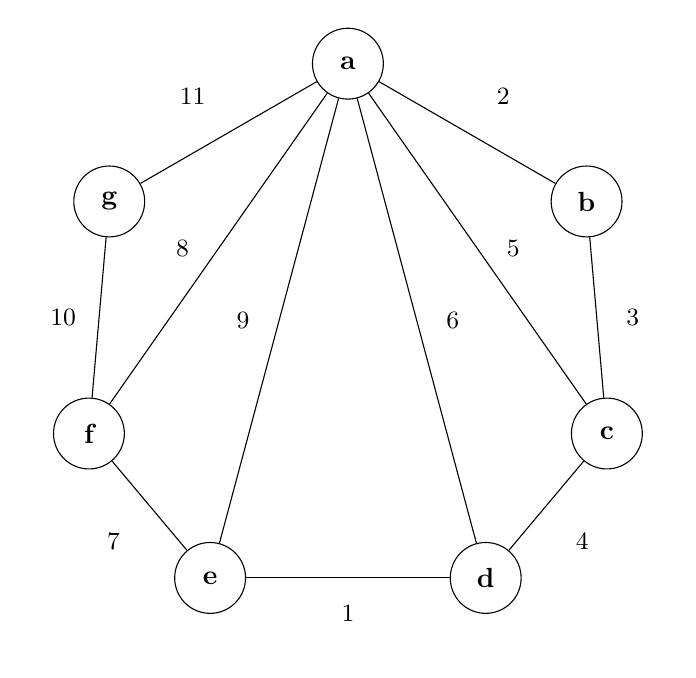
\begin{tikzpicture}[
    every node/.style={circle, draw, minimum size=0.9cm, font=\bfseries},
    edge label/.style={rectangle, draw=none,  font=\normalfont\small},
  ]

  % Center node
  \node (a) at (90:3.5)  {a};  % top

  % Outer ring (clockwise)
  \node (b) at (30:3.5)   {b};
  \node (c) at (-20:3.5)  {c};
  \node (d) at (-60:3.5)  {d};
  \node (e) at (-120:3.5) {e};
  \node (f) at (-160:3.5) {f};
  \node (g) at (150:3.5)  {g};

  % Outer polygon edges
  \draw (a) -- node[edge label, above right] {2}  (b);
  \draw (b) -- node[edge label, right]       {3}  (c);
  \draw (c) -- node[edge label, below right] {4}  (d);
  \draw (d) -- node[edge label, below]       {1}  (e);
  \draw (e) -- node[edge label, below left]  {7}  (f);
  \draw (f) -- node[edge label, left]        {10} (g);
  \draw (g) -- node[edge label, above left]  {11} (a);

  % Spokes (center to outer)
  \draw (a) -- node[edge label, right]       {5}  (c);
  \draw (a) -- node[edge label, right]       {6}  (d);
  \draw (a) -- node[edge label, left]        {8}  (f);
    \draw (a) -- node[edge label, left]        {9}  (e);

  \end{tikzpicture}

\end{center}
%% ================= GLOBAL DEFINITIONS FOR KRUSKAL'S GRAPH =================
%% TikZ Styles
\tikzset{
  stepnode/.style={circle, draw=black!70, thick, minimum size=0.65cm, font=\bfseries, fill=white, inner sep=1pt},
  mstedge/.style={very thick, blue},
  edgelbl/.style={draw=none, fill=white, font=\small\bfseries, text=black, inner sep=1pt},
  grayedge/.style={-, color=black!15, line width=0.8pt},
  graylbl/.style={draw=none, fill=white, font=\scriptsize, inner sep=1pt, text=black!30}
}

%% Graph Nodes and Faint Edges (Global Definitions)
\gdef\drawKruskalNodes{
  \node[stepnode] (a) at (90:3.5)  {a};
  \node[stepnode] (b) at (30:3.5)  {b};
  \node[stepnode] (c) at (-20:3.5) {c};
  \node[stepnode] (d) at (-60:3.5) {d};
  \node[stepnode] (e) at (-120:3.5){e};
  \node[stepnode] (f) at (-160:3.5){f};
  \node[stepnode] (g) at (150:3.5) {g};
}

\gdef\drawKruskalFaintEdges{
  \draw[grayedge] (a) -- node[graylbl, above right] {2}  (b);
  \draw[grayedge] (b) -- node[graylbl, right]       {3}  (c);
  \draw[grayedge] (c) -- node[graylbl, below right] {4}  (d);
  \draw[grayedge] (d) -- node[graylbl, below]       {1}  (e);
  \draw[grayedge] (e) -- node[graylbl, below left]  {7}  (f);
  \draw[grayedge] (f) -- node[graylbl, left]        {10} (g);
  \draw[grayedge] (g) -- node[graylbl, above left]  {11} (a);
  \draw[grayedge] (a) -- node[graylbl, right, pos=0.7] {5}  (c);
  \draw[grayedge] (a) -- node[graylbl, right, pos=0.8] {6}  (d);
  \draw[grayedge] (a) -- node[graylbl, left, pos=0.8]  {8}  (f);
  \draw[grayedge] (a) -- node[graylbl, left, pos=0.7]  {9}  (e);
}
%% =========================================================================

\item Construct the Huffman tree and show the Huffman coding for the following characters with given frequencies:
\begin{center}
\begin{tabular}{ccccccc}
\toprule
Character & a & b & c & d & e & f \\
\midrule
Frequency & 50 & 30 & 20 & 15 & 10 & 5 \\
\bottomrule
\end{tabular}
\end{center}
\mk{10}
\yr{CSE 207 | 2009--10}
%% ---------------------------------------------------------------------
%% Q: Huffman tree for a:50,b:30,c:20,d:15,e:10,f:5.
%%    [CSE 207 | 2009--10]   ← Python verified \checkmark{}   total=305 bits
%% ---------------------------------------------------------------------

\item Construct a minimum spanning tree using Kruskal's algorithm for the following weighted graph: $AB(2), AC(3), AE(5), BC(1), BD(6), BF(9), CF(3), CG(2), DE(7),\\ DH(5), FG(4)$. Show every step, giving reasons for discarding any edge. \mk{15+5=20}
\yr{CSE 207 | 2008--09}

%% ================= GLOBAL DEFINITIONS FOR NEW KRUSKAL'S GRAPH =================
%% TikZ Styles (If not already defined)
\tikzset{
  stepnode/.style={circle, draw=black!70, thick, minimum size=0.65cm, font=\bfseries, fill=white, inner sep=1pt},
  mstedge/.style={very thick, blue},
  edgelbl/.style={draw=none, fill=white, font=\small\bfseries, text=black, inner sep=1pt},
  grayedge/.style={-, color=black!15, line width=0.8pt},
  graylbl/.style={draw=none, fill=white, font=\scriptsize, inner sep=1pt, text=black!30}
}

%% Graph Nodes and Faint Edges (Global Definitions)
\gdef\drawKruskalNodesEight{
  \node[stepnode] (A) at (2, 4)  {A};
  \node[stepnode] (B) at (0, 2)  {B};
  \node[stepnode] (C) at (4, 2)  {C};
  \node[stepnode] (D) at (-2, 0) {D};
  \node[stepnode] (E) at (0, 5)  {E};
  \node[stepnode] (F) at (4, 0)  {F};
  \node[stepnode] (G) at (6, 3)  {G};
  \node[stepnode] (H) at (-2, -2){H};
}

\gdef\drawKruskalFaintEdgesEight{
  \draw[grayedge] (B) -- node[graylbl, below]       {1} (C);
  \draw[grayedge] (A) -- node[graylbl, above left]  {2} (B);
  \draw[grayedge] (C) -- node[graylbl, below right] {2} (G);
  \draw[grayedge] (C) -- node[graylbl, right]       {3} (F);
  \draw[grayedge] (A) -- node[graylbl, above right] {3} (C);
  \draw[grayedge] (F) -- node[graylbl, right]       {4} (G);
  \draw[grayedge] (A) -- node[graylbl, right]       {5} (E);
  \draw[grayedge] (D) -- node[graylbl, left]        {5} (H);
  \draw[grayedge] (B) -- node[graylbl, above left]  {6} (D);
  \draw[grayedge] (D) -- node[graylbl, left]        {7} (E);
  \draw[grayedge] (B) -- node[graylbl, below left, pos=0.8] {9} (F);
}
%% ==============================================================================

\item Discuss how Prim's algorithm constructs a minimum spanning tree. Argue how sets and the disjoint-set union algorithm can be used to detect cycles and improve upon Kruskal's algorithm. \mk{15}
\yr{CSE 207 | 2008--09}

\item Discuss how a Huffman tree can be constructed given a sequence of frequencies corresponding to symbols. Construct a dynamic Huffman tree based upon the message \texttt{ABBBCAAAACBBBB}. \mk{20}
\yr{CSE 207 | 2008--09}

\item Suppose you have a washing machine that a number of users want to use. Each user $i$ sends a request for the time interval $(s_i, f_i)$ (start and finish times). The machine can serve only one user at a time, and each user pays 1000/- regardless of duration. Write a greedy algorithm to maximize revenue. Prove the correctness of your algorithm and deduce its running time. \mk{8+10+5}
\yr{CSE 207 | 2007--08}
%% ---------------------------------------------------------------------
%% Q: Washing machine scheduling = Activity Selection Problem.
%%    [CSE 207 | 2007--08]
%% ---------------------------------------------------------------------

\item Define the interval coloring problem and write an algorithm to solve it. \mk{4+8}
\yr{CSE 207 | 2007--08}
%% ---------------------------------------------------------------------
%% Q: Interval coloring problem --- definition + algorithm.
%%    [CSE 207 | 2007--08]
%% ---------------------------------------------------------------------

\item Describe the main idea of Prim's algorithm to compute a minimum spanning tree. Discuss how Prim's algorithm can be implemented in $O(m \log n)$ time. Discuss the reverse-delete algorithm to compute a minimum spanning tree and prove its correctness. \mk{6+10+17}
\yr{CSE 207 | 2007--08}
%% ---------------------------------------------------------------------
%% Q: Prim's idea; O(m log n) implementation; reverse-delete.
%%    [CSE 207 | 2007--08]
%% ---------------------------------------------------------------------

\item Write down an algorithm for constructing a minimum spanning tree using Kruskal's algorithm. Show how sets and the disjoint-set algorithm can be used to reduce its complexity. Construct a minimum spanning tree for the graph with edges: $AB(7), AC(3), DA(4), EA(1), BC(91), CF(9), BD(7), EB(2), FB(5), CE(4), DE(6),\\ FD(3)$. \mk{5+5+5}
\yr{CSE 207 | 2006--07}

%% ================= GLOBAL DEFINITIONS FOR THIRD KRUSKAL GRAPH =================
%% TikZ Styles (If not already defined)
\tikzset{
  stepnode/.style={circle, draw=black!70, thick, minimum size=0.65cm, font=\bfseries, fill=white, inner sep=1pt},
  mstedge/.style={very thick, blue},
  edgelbl/.style={draw=none, fill=white, font=\small\bfseries, text=black, inner sep=1pt},
  grayedge/.style={-, color=black!15, line width=0.8pt},
  graylbl/.style={draw=none, fill=white, font=\scriptsize, inner sep=1pt, text=black!30}
}

%% Graph Nodes (MUST BE DRAWN FIRST TO PREVENT ALIGNMENT BUGS)
\gdef\drawKruskalNodesSix{
  \node[stepnode] (A) at (90:3.5)  {A};
  \node[stepnode] (B) at (30:3.5)  {B};
  \node[stepnode] (F) at (-30:3.5) {F};
  \node[stepnode] (D) at (-90:3.5) {D};
  \node[stepnode] (E) at (-150:3.5){E};
  \node[stepnode] (C) at (150:3.5) {C};
}

%% Faint Edges
\gdef\drawKruskalFaintEdgesSix{
  \draw[grayedge] (A) -- node[graylbl, above right] {7} (B);
  \draw[grayedge] (A) -- node[graylbl, above left]  {3} (C);
  \draw[grayedge] (D) -- node[graylbl, right, pos=0.8] {4} (A);
  \draw[grayedge] (E) -- node[graylbl, left, pos=0.8]  {1} (A);
  \draw[grayedge] (B) -- node[graylbl, above, pos=0.25] {91}(C);
  \draw[grayedge] (C) -- node[graylbl, below, pos=0.2]  {9} (F);
  \draw[grayedge] (B) -- node[graylbl, left, pos=0.8]   {7} (D);
  \draw[grayedge] (E) -- node[graylbl, above, pos=0.25] {2} (B);
  \draw[grayedge] (F) -- node[graylbl, right]           {5} (B);
  \draw[grayedge] (C) -- node[graylbl, left]            {4} (E);
  \draw[grayedge] (D) -- node[graylbl, below left]      {6} (E);
  \draw[grayedge] (F) -- node[graylbl, below right]     {3} (D);
}
%% ==============================================================================

\item Construct a Huffman tree for the phrase with symbols and frequencies: $A$-7, $B$-4, $C$-5, $D$-2, $E$-20, $F$-3, $G$-6, $H$-8, $I$-1. \mk{10}
\yr{CSE 207 | 2006--07}

\item There is a set of jobs where each job has an integer deadline and profit, and only one machine is available. To complete a job requires one unit of time; profit is earned only if the job is completed by its deadline. Jobs $A, B, C, D, E$ have deadlines $3, 3, 1, 2, 2$ and profits $1, 5, 10, 15, 20$ respectively. Show the steps of selecting jobs using a greedy strategy. \mk{8}
\yr{CSE 207 | 2006--07}
%% ---------------------------------------------------------------------
%% Q: Job sequencing A(d=3,p=1),B(d=3,p=5),C(d=1,p=10),D(d=2,p=15),E(d=2,p=20).
%%    [CSE 207 | 2006--07]   ← Python verified \checkmark{}  Total profit = 40
%% ---------------------------------------------------------------------

\item Find the shortest paths starting from vertex $s$ in this given graph. Show the steps of edge relaxation. \mk{10}
\yr{CSE 207 | 2006--07}

\begin{center}
  
\includegraphics[height=0.25\textheight, width=0.75\textwidth,keepaspectratio]{/159.png}
\end{center}

%% ══════════════════════════════════════════════════════════════════════
%% ANSWER SNIPPETS --- Greedy Algorithms, MST, Dijkstra, Huffman, Knapsack
%% ALL simulation results verified by Python before writing LaTeX.
%% ══════════════════════════════════════════════════════════════════════

\item Once an amateur thief entered into a museum full of tantalizing jewelry,
geodes and rare gems. As he is new in this field, he brought just a single
backpack with him that has a capacity of 6\,kg. The thief planned to get away
with the most valuable objects without overloading the backpack. He found out
that in a less-secured compartment, there were four (4) solid items, and their
information are given in the following table.

\begin{center}
\begin{tabular}{|l|c|c|}
\hline
\textbf{Item} & \textbf{Weight (kg)} & \textbf{Value (USD)} \\
\hline
Brooch of the queen & 3  & 15 \\
Crown of the king   & 2  & 20 \\
Decorated vase      & 10 & 30 \\
An ancient coin     & 2  & 14 \\
\hline
\end{tabular}

\smallskip
\small Table for Ques No.~5(a) --- Information of valuable items found in the museum
\end{center}

Since the items are unbreakable, for each item, the thief must pick the whole
of it or not consider it at all. Now although our thief is amateur in this
business, he possesses some algorithmic knowledge. Therefore, he applied a
greedy technique and selected the items that gave him the maximum possible
profit per weight, and then he left the museum with so much zeal! Now, using
the information of the backpack of the thief and the item table given for this
question, your first task is to show the steps of finding the maximum possible
profit and the corresponding list of items using the technique that the thief
adopted. You have also identified that the scenario at the museum was a special
one and only dynamic programming is able to find the optimal solution in that
case. Therefore, your second task is to find the optimal profit and the list of
items using dynamic programming. \mk{10+10=20}

\end{enumerate}
\newpage

\secdivider{Dynamic Programming}{LCS, MCM, Edit Distance, Knapsack, Memoization}{cD}{cD}
\markboth{T11 --- Dynamic Programming}{}
\label{sec:T11}
\section{T11 --- Dynamic Programming}

\begin{enumerate}
\item Assume that you have obtained a gold bar of integer length $n$. You plan to cut it into smaller pieces and sell them to the market. For any integer $i \leq n$, you know the profit you will obtain if you sell a gold bar of length $i$.
\begin{enumerate}
  \item Using the cut-and-paste method, formulate an argument to show that the problem of obtaining the maximum profit by cutting this gold bar into smaller pieces has the optimal substructure property.
  \item Construct a recursion tree diagram to show that the problem has the overlapping subproblem property.
\end{enumerate}
\mk{7+8=15}
\yr{CSE 105 | 2023--24}

\item Given the two strings $X = \texttt{``AGGTAB''}$ and $Y = \texttt{``GXTYAB''}$, construct the dynamic programming (DP) table to compute the length of the Longest Common Subsequence (LCS) between $X$ and $Y$. Clearly state the LCS and its length. \mk{15}
\yr{CSE 105 | 2023--24}

\item You are given a sequence of matrices $\langle A_1, A_2, \ldots, A_n \rangle$ and their dimensions $\langle p_0, p_1, p_2, \ldots, p_n \rangle$ such that matrix $A_i$ has dimensions $p_{i-1} \times p_i$. The matrix-chain multiplication (MCM) problem aims to identify the minimum number of scalar multiplications necessary to compute the product of the given chain of matrices. Formulate a recurrence relation to solve this problem. Design an efficient dynamic programming algorithm using the recurrence relation. \mk{15}
\yr{CSE 105 | 2023--24}

\item You are given a sequence of matrices $\langle A_1, A_2, \ldots, A_n \rangle$ and their dimensions $\langle p_0, p_1, p_2, \ldots, p_n \rangle$ such that matrix $A_i$ has dimensions $p_{i-1} \times p_i$. The matrix-chain multiplication (MCM) problem aims to identify the minimum number of scalar multiplications necessary to determine the product of the given chain of matrices.
\begin{enumerate}
  \item Formulate arguments to show that the MCM problem has the optimal substructure property.
  \item Compose a recursion tree diagram to show that MCM has the overlapping subproblem property.
  \item Design an efficient algorithm using the dynamic programming approach to solve this problem.
\end{enumerate}
\mk{8+7+10=25}
\yr{CSE 105 | 2022--23}

%% -- Q6 --------------------------------------------------------------

\item Using a dynamic programming algorithm, determine the minimum edit distance alignment of the two strings $X = \texttt{ATCGGT}$ and $Y = \texttt{ACCDT}$, where both the gap penalty and mismatch penalty are 1 and the cost of a match is 0. Show the DP table, the alignments, and mark the paths (which correspond to the alignments) in the DP table. \mk{10}
\yr{CSE 105 | 2022--23}

\item Given two strings, the longest common subsequence (LCS) problem is to find the longest subsequence present in both strings in the same relative order, but not necessarily contiguous. For example, for $S_1 = \texttt{``ALGORITHM''}$ and $S_2 = \texttt{``LITHIUM''}$, the LCS is \texttt{``LITHM''}. Present a dynamic programming algorithm to find the length of the LCS of two strings. Derive a proof of correctness of the algorithm and also derive its running time. \mk{8+6+3=17}
\yr{CSE 105 | 2021--22}

%% -- Q5 --------------------------------------------------------------

\item Solve the following 0-1 knapsack problem instance (capacity = 6) using dynamic programming. Show the DP table and find the optimal set of items.
\begin{center}
\begin{tabular}{ccc}
\toprule
Item & Weight & Value \\
\midrule
1 & 2 & 8 \\
2 & 1 & 7 \\
3 & 2 & 12 \\
4 & 2 & 6 \\
5 & 2 & 10 \\
\bottomrule
\end{tabular}
\end{center}
\mk{15}
\yr{CSE 203 | 2021--22}

%% ---------------------------------------------------------------------
%% Q: 0-1 Knapsack cap=6, items (2,8),(1,7),(2,12),(2,6),(2,10).
%%    [CSE 203 | 2021--22]   ← Python verified \checkmark{}
%%    Optimal: items 1,3,5; value=30; weight=6
%% ---------------------------------------------------------------------

\item Find the best alignment (minimum edit distance) of the following two DNA sequences using dynamic programming. Use gap penalty = 3, mismatch penalty = 2, match penalty = 0. Show the DP table, the alignment, and mark the corresponding path.
\[ \texttt{CCAGTGC} \quad \text{vs} \quad \texttt{CGATC} \]
\mk{15}
\yr{CSE 203 | 2021--22}
%% ---------------------------------------------------------------------
%% Q: Sequence alignment CCAGTGC vs CGATC (gap=3,mismatch=2,match=0).
%%    [CSE 203 | 2021--22]   ← Python verified \checkmark{}   dist=8
%% ---------------------------------------------------------------------

\item Give a dynamic programming algorithm to find the length of the longest common subsequence (LCS) of two strings. (A common subsequence appears in both strings in the same relative order but not necessarily contiguously.) \mk{20}
\yr{CSE 203 | 2021--22}
%% ---------------------------------------------------------------------
%% Q: LCS algorithm (general).  [CSE 203 | 2021--22]
%% ---------------------------------------------------------------------

\item Derive a recursive definition to find $m[i,j]$ (the minimum number of multiplications to compute $A_i \cdot A_{i+1} \cdots A_j$). With a recursion tree, describe the overlapping sub-problem property of Matrix Chain Multiplication (MCM). Then, given six matrices $A_1(30\times35)$, $A_2(35\times15)$, $A_3(15\times5)$, $A_4(5\times10)$, $A_5(10\times20)$, $A_6(20\times25)$ and the following partial DP table, give an ordering to populate the marked cells and calculate $m[2,5]$:
\begin{center}
\begin{tabular}{c|cccccc}
\toprule
 & 1 & 2 & 3 & 4 & 5 & 6 \\
\midrule
1 & 0 & 15750 & 7875 & $m[1,4]$ & $m[1,5]$ & $m[1,6]$ \\
2 & & 0 & 2625 & 4375 & $m[2,5]$ & $m[2,6]$ \\
3 & & & 0 & 750 & 2500 & $m[3,6]$ \\
4 & & & & 0 & 1000 & $m[4,6]$ \\
5 & & & & & 0 & $m[5,6]$ \\
6 & & & & & & 0 \\
\bottomrule
\end{tabular}
\end{center}
\mk{7+6+10}
\yr{CSE 203 | 2020--21}

\item At the beginning of the COVID-19 pandemic, two biologists were identifying the similarity between COVID-19 and SARS viruses using genome sequences $S_1' = \langle A,T,T,G,C,A,T \rangle$ and $S_2' = \langle T,A,G,C,C,T \rangle$.
\begin{enumerate}
  \item (Dr.\ Brown's task) Write the recursive definition for the Longest Common Subsequence (LCS) problem and populate the DP table with arrows showing how cell values propagate. Find the length and the LCS itself.
  \item (Dr.\ William's task) Write the recursive definition for the edit distance problem using operations \{Insert (cost 1), Delete (cost 1), Replacement (cost 1), Keep (cost 0)\}. Populate the DP table and show the edit distance cost and sequence of required operations.
\end{enumerate}
\mk{15}
\yr{CSE 203 | 2020--21}

\item Discuss a problem scenario where adopting memoization over bottom-up dynamic programming can result in a faster solution. Justify your answer. \mk{5}
\yr{CSE 203 | 2020--21}
%% ---------------------------------------------------------------------
%% Q: Memoization vs bottom-up DP.  [CSE 203 | 2020--21]
%% ---------------------------------------------------------------------

\item Apply dynamic programming to calculate the edit distance of the following two DNA sequences, where the cost of insertion or deletion is 2 and the cost of substitution is 1. Write the recurrence relation, explain the intuition behind it, populate the DP table, and calculate the edit distance.
\[ \texttt{TGCATAT} \quad \text{vs} \quad \texttt{ATCCGA} \]
\mk{15}
\yr{CSE 203 | 2019--20}

%% -- Q1 --------------------------------------------------------------

\item Briefly explain the steps to be followed for solving a problem using dynamic programming. \mk{10}
\yr{CSE 203 | 2018--19}

\item Dream coins are used by the people of Dreamland. Only the following coins are available: \$1, \$7, \$11, and \$15.
\begin{enumerate}
  \item Write an example of an amount where the greedy strategy for the Coin-Change problem does \emph{not} provide an optimal solution. Mention both the greedy and optimal solutions.
  \item Using dynamic programming, find the minimum number of coins that add up to \$20.
\end{enumerate}
\mk{10}
\yr{CSE 203 | 2018--19}

\item Consider the following 0/1 knapsack problem instance (capacity = 7):
\begin{center}
\begin{tabular}{ccc}
\toprule
Item & Weight & Value \\
\midrule
1 & 1 & 50 \\
2 & 3 & 60 \\
3 & 5 & 100 \\
4 & 2 & 70 \\
5 & 2 & 80 \\
\bottomrule
\end{tabular}
\end{center}
Solve this instance using dynamic programming. Show the DP table and find all solutions using the table. \mk{15}
\yr{CSE 203 | 2018--19}

\item Find all longest common subsequences of $X = \langle T,A,A,G,U,A,T,U \rangle$ and $Y = \langle A,U,A,G,T,U,T \rangle$ using dynamic programming. Also find a shortest common supersequence of $X$ and $Y$ using an LCS of $X$ and $Y$. \mk{15}
\yr{CSE 203 | 2018--19}

\item Suppose you run a bus lending business, and each request has the format (start time, end time). Find all solutions for the maximum number of requests that can be satisfied by:
\begin{enumerate}
  \item Earliest start time
  \item Shortest interval
  \item Earliest end time
\end{enumerate}
Use the following requests: $\{[1,6),[4,8),[6,8),[9,15),[6,9),[11,15),[2,6)\}$.\\
\mk{12}
\yr{CSE 203 | 2018--19}

\item Let $A_1(11\times4)$, $A_2(4\times5)$, $A_3(5\times3)$, $A_4(3\times6)$, $A_5(6\times7)$, $A_6(7\times1)$ be six matrices. Compute $m[1,6]$ given: $m[1,3]=35$, $m[2,4]=132$, $m[1,5]=95$, $m[2,5]=270$, $m[2,6]=95$, $m[4,5]=126$, $m[4,6]=60$. \mk{13}
\yr{CSE 203 | 2018--19}

\item Briefly explain with examples: (i) Optimal substructure, and (ii) Overlapping subproblems. Then recall the divide-and-conquer algorithm for merge sort and analyze its running time. \mk{8+7}
\yr{CSE 203 | 2017--18}

\item Consider the following instance of the 0-1 knapsack problem (capacity = 6):
\begin{center}
\begin{tabular}{ccc}
\toprule
Item & Weight & Value \\
\midrule
1 & 2 & 7 \\
2 & 1 & 8 \\
3 & 2 & 12 \\
4 & 2 & 6 \\
5 & 2 & 10 \\
\bottomrule
\end{tabular}
\end{center}
Solve this instance using dynamic programming. Show the DP table and find the optimal set of items from the table. \mk{15}
\yr{CSE 203 | 2017--18}

\item Given two strings, the longest common \emph{substring} problem is to find the longest string that is a substring of both given strings. For example, for $S_1 = \texttt{buetcserocks}$ and $S_2 = \texttt{bdcserocks}$, the longest common substring is \texttt{cserocks}. Give a dynamic programming algorithm to find the length of the longest common substring. \mk{15}
\yr{CSE 203 | 2017--18}

\item Solve the following instance of the 0-1 knapsack problem using a branch-and-bound algorithm with a state-space tree (capacity = 10\,kg):
\begin{center}
\begin{tabular}{cccc}
\toprule
Item & Weight (kg) & Profit (Taka) \\
\midrule
1 & 3 & 18 \\
2 & 5 & 35 \\
3 & 4 & 44 \\
4 & 7 & 36 \\
5 & 2 & 18 \\
\bottomrule
\end{tabular}
\end{center}
\mk{8}
\yr{CSE 207 | 2017--18}

\item Recall the Weighted Interval Scheduling Problem. You are given $n$ intervals with starting time $s_i$, finishing time $f_i$, and value $v_i$. A subset of intervals is compatible if no two overlap. Give a dynamic programming algorithm to find a compatible subset maximizing $\sum_{i \in S} v_i$. Your algorithm (including preprocessing) should run in $O(n \log n)$ time. \mk{15}
\yr{CSE 203 | 2016--17}

\item Consider the following Boolean formula: $(x' \vee y)(x \vee y' \vee z)(y \vee y')(x \vee y)(x \vee y \vee z')(x \vee y \vee z)$. Use a backtracking algorithm to decide whether it is satisfiable. Show the backtracking tree. \mk{15}
\yr{CSE 207 | 2016--17}

\item Solve the following 0-1 knapsack instance (capacity = 10) using the branch-and-bound algorithm. Show the branch-and-bound tree.
\begin{center}
\begin{tabular}{ccc}
\toprule
Item & Weight & Value \\
\midrule
1 & 2 & 10 \\
2 & 3 & 9 \\
3 & 2 & 20 \\
4 & 5 & 30 \\
\bottomrule
\end{tabular}
\end{center}
\mk{20}
\yr{CSE 207 | 2016--17}

\item What is the matrix chain multiplication problem? Prove that it has both the overlapping subproblems property and the optimal substructure property. \mk{10}
\yr{CSE 207 | 2015--16}

\item Write the steps to be followed for solving a problem using dynamic programming. Let $X = (x_1, \ldots, x_m)$ and $Y = (y_1, \ldots, y_n)$ be sequences, and let $Z = (z_1, \ldots, z_k)$ be any LCS of $X$ and $Y$. If $x_m \neq y_n$ and $z_k \neq x_m$, prove that $Z$ is an LCS of $X_{m-1}$ and $Y$. \mk{4+6=10}
\yr{CSE 207 | 2015--16}

\item Find all longest common subsequences of $X = \langle A,G,G,C,T,G,A,T \rangle$ and $Y = \langle G,G,G,C,A,T,A \rangle$ using dynamic programming. \mk{15}
\yr{CSE 207 | 2015--16}

\item Solve the following 0/1 knapsack instance (capacity = 15) using the branch-and-bound approach with a state-space tree:
\begin{center}
\begin{tabular}{ccc}
\toprule
Item & Weight & Value \\
\midrule
1 & 7 & 140 \\
2 & 6 & 132 \\
3 & 4 & 140 \\
4 & 3 & 90 \\
\bottomrule
\end{tabular}
\end{center}
Compare the backtracking and branch-and-bound techniques. \mk{3+12=15}
\yr{CSE 207 | 2015--16}

\item What are the key properties of an optimization problem that allow it to be solved using dynamic programming? Compare top-down memoized DP with bottom-up DP, and identify types of problems for which one outperforms the other. \mk{12}
\yr{CSE 207 | 2014--15}

\item The balanced partition problem: given $n$ integers each in $[0, N]$, divide them into two subsets minimizing the difference of their sums (e.g., for $S = \{1,7,3,5,9\}$, a balanced partition is $S_1 = \{1,7,5\}$ and $S_2 = \{3,9\}$ with difference 1). Formulate a dynamic programming solution and determine its time complexity. \mk{12}
\yr{CSE 207 | 2014--15}

\item Using dynamic programming, compute the minimum number of scalar multiplications for the matrix chain multiplication of $A_1, A_2, A_3, A_4, A_5, A_6$ with dimensions $15\times5$, $5\times50$, $50\times20$, $20\times10$, $10\times35$, $35\times25$. Also show the ordering of the matrices for the minimum. \mk{15}
\yr{CSE 207 | 2013--14}

%% ---------------------------------------------------------------------
%% Q: Matrix Chain A1-A6 (15x5,5x50,50x20,20x10,10x35,35x25).
%%    [CSE 207 | 2013--14]   ← Python verified \checkmark{}   cost=14000
%% ---------------------------------------------------------------------

\item Compare dynamic programming and memoization techniques. ``A dynamic programming algorithm usually outperforms the corresponding memoized algorithm'' --- explain. \mk{10}
\yr{CSE 207 | 2013--14}

\item Write a memoized algorithm for solving the matrix chain multiplication problem. Analyze its time complexity. \mk{10}
\yr{CSE 207 | 2013--14}

\item What is a state-space tree? Solve the following instance of the 0/1 knapsack problem (capacity = 10) using the branch-and-bound approach with a state-space tree:
\begin{center}
\begin{tabular}{ccc}
\toprule
Item & Weight & Value \\
\midrule
1 & 7 & 42 \\
2 & 4 & 40 \\
3 & 3 & 12 \\
4 & 5 & 25 \\
\bottomrule
\end{tabular}
\end{center}
\mk{15}
\yr{CSE 207 | 2013--14}

\item Prove that the longest common subsequence problem has both the Overlapping Subproblems property and the Optimal Substructure property. \mk{10}
\yr{CSE 207 | 2013--14}

%% ---------------------------------------------------------------------
%% Q: LCS properties (overlapping + optimal substructure).
%%    [CSE 207 | 2013--14]
%% ---------------------------------------------------------------------

\item Find all longest common subsequences of $X = \langle A,T,G,C,T,G,A,T \rangle$ and $Y = \langle T,G,G,C,A,T,A \rangle$ using dynamic programming. \mk{15}
\yr{CSE 207 | 2013--14}

\item In a previous life, you worked as a cashier in the ancient city of Egypt, spending the better part of your day giving change to your customers. Because paper was a very rare and valuable resource at the time, cashiers were required by law to use the fewest notes possible whenever they gave change. The currency of Egypt at that time, called Dream Dollars, was available in the following denominations: \$1, \$4, \$7, \$13, \$28, \$52, \$91, \$365. \mk{20}
\begin{enumerate}
  \item A greedy change algorithm repeatedly takes the largest note that does not exceed the target amount. For example, to make \$122 using the greedy algorithm, we first take a \$91 note, then a \$28 note, and finally three \$1 notes. Give an example where this greedy algorithm uses more Dream Dollar notes than the minimum possible.
  \item Describe a dynamic programming algorithm that computes, given an integer $k$, the minimum number of notes needed to make $k$ Dream Dollars. Write down the pseudocodes for both the memoized approach and bottom-up iterative approach. Analyze the running-times of both approaches.
\end{enumerate}
\yr{CSE 207 | 2012--13}
%% ---------------------------------------------------------------------
%% Q: Coin change (Dream Dollars) --- greedy counterexample + DP.
%%    [CSE 207 | 2012--13]
%%    No counterexample found for these specific denominations
%%    up to 200 --- greedy appears optimal here; note this.
%% ---------------------------------------------------------------------

\item You have $n$ magic boxes kept in a row, numbered 1 to $n$, each containing some dollars. You can open box $i$ only if you did not open box $i-1$ or box $i-2$. Given the amount $D[1 \ldots n]$ in each box, find the maximum dollars obtainable. Describe a dynamic programming solution and analyze its running time. \mk{12}
\yr{CSE 207 | 2012--13}
%% ---------------------------------------------------------------------
%% Q: Magic boxes --- max non-adjacent sum.  [CSE 207 | 2012--13]
%%    ← Python verified \checkmark{}   D=[1,9,3,7,5,2,8,4] $\rightarrow$ max=24
%% ---------------------------------------------------------------------

\item Suppose we are given a sequence of integers $A[1..n]$ and we want to find the longest subsequence whose elements are in decreasing order. More concretely, we want to find the longest sequence of indices $1 < i_1 < i_2 < \ldots < i_k < n$ such that $A[i_j] > A[i_{j+1}]$ for all $j$. Describe the pseudocode of a backtracking algorithm that solves this problem in $O(2^n)$ time. \mk{15}
\yr{CSE 207 | 2012--13}

\item Compare the properties of problems that can be solved with the greedy method, divide-and-conquer method, and dynamic programming method. \mk{3}
\yr{CSE 207 | 2011--12}

\item Write and prove the optimal-substructure property of the matrix chain multiplication problem. Calculate the number of parenthesizations of a sequence of $n$ matrices. \mk{5+5=10}
\yr{CSE 207 | 2011--12}

%%---------------------------------------------------------------------
\item Find an optimal solution to the 0/1 knapsack instance of $n = 4$,
$W = 6$, $(v_1,v_2,v_3,v_4)=(50,30,12,45)$,
$(w_1,w_2,w_3,w_4)=(2,3,1,3)$. \mk{15}
\yr{CSE 207 | 2011--12}

\item Let $X = (x_1, x_2, \ldots, x_m)$ and $Y = (y_1, y_2, \ldots, y_n)$ be sequences, and let $Z = (z_1, z_2, \ldots, z_k)$ be any LCS of $X$ and $Y$. If $x_m \neq y_n$ and $z_k \neq x_m$, prove that $Z$ is an LCS of $X_{m-1}$ and $Y$. \mk{2}
\yr{CSE 207 | 2011--12}

\item Find an LCS of $X = \langle A,T,C,T,G,A,T \rangle$ and $Y = \langle T,G,C,A,T,A \rangle$ by showing the $c$ and $b$ tables. \mk{10}
\yr{CSE 207 | 2011--12}

%% ---------------------------------------------------------------------
\item Give an example of a problem that has the optimal substructure property. Give another example of a problem that does not have optimal substructure. Justify your answers. \mk{10}
\yr{CSE 207 | 2009--10}

\item Show the execution of the Dynamic Programming LCS algorithm for the following two strings: $X = \langle A,B,C,B \rangle$ and $Y = \langle B,D,A,C \rangle$. \mk{15}
\yr{CSE 207 | 2009--10}

\item Show all the different ways to multiply the matrix chain $A_1 A_2 A_3 A_4 A_5$. \mk{5}
\yr{CSE 207 | 2009--10}

\item Convert the following recursive procedure for computing the $n$-th Fibonacci number into an equivalent procedure that uses a dynamic multi-graph representing the computation. From this graph, find $T_1(5)$, $T_\infty(5)$, and the parallelism.
\begin{verbatim}
F(n)
  if n <= 1 then return n
  else return F(n-1) + F(n-2)
\end{verbatim}
\mk{17}
\yr{CSE 207 | 2009--10}

\item Find a longest common subsequence from the DNA sequences \texttt{ACGCTAC} and \texttt{CTGCA}. Print the sequence also. Analyze the run times of your methods of finding and printing the sequence. \mk{10+5=15}
\yr{CSE 207 | 2008--09}

\item Find the optimal sequence of multiplying the following matrices: $A(2\times7)$, $B(7\times9)$, $C(9\times4)$, $D(4\times6)$, $E(6\times3)$. How does the memoization technique help? \mk{10+5=15}
\yr{CSE 207 | 2008--09, 2006--07}

\item Mention the basic properties that must be satisfied to solve a problem using dynamic programming. When and how can memoization help improve an exponential-time recursive algorithm to polynomial time? \mk{7+8}
\yr{CSE 207 | 2007--08}
%% ---------------------------------------------------------------------
%% Q: DP properties; memoization transforms exponential to polynomial.
%%    [CSE 207 | 2007--08]
%% ---------------------------------------------------------------------

\item Suppose a thief went to a superstore to steal. He has a bag with him which can contain at most $W$ unit of weight of anything. The thief can carry at most $W'$ unit of weight. In the store there are two types of things. For Type 1 things, he either has to take the thing or leave it. For Type 2 things, he can weigh and take as per his will (e.g.\ sugar, rice, salt etc.). All type 1 things are labeled with the corresponding unit prices and each type 2 thing is labeled with the corresponding price per unit weight. The thief decided to take only the things belonging to Type 1. He now needs an algorithm to maximize his profits.
\begin{enumerate}
  \item Map the above problem to one of your known problems. \mk{5}
  \item Discuss possible greedy strategies to solve the problem and discuss whether or not any of them will work. \mk{7}
  \item If the thief decides to take only type 2 things, will any of the greedy strategies work? Justify your answer. \mk{6}
\end{enumerate}

\yr{CSE 207 | 2007--08}
%% ---------------------------------------------------------------------
%% Q: Thief problem --- Type 1 = 0-1 Knapsack, Type 2 = Fractional.
%%    [CSE 207 | 2007--08]
%% ---------------------------------------------------------------------

\item Find an optimal solution to the 0--1 knapsack problem with the following weight and profit values (weight limit = 8):
$(1,2),\ (1,3),\ (2,3),\ (2,5),\ (3,4),\ (3,2),\ (3,7)$.
\mk{10}
\yr{CSE 207 | 2006--07}

\item Construct four matrices for finding all-pairs shortest paths for a given graph (edges: $AB(7), AC(3), DA(4), EA(1), BC(91), CF(9), BD(7), EB(2), FB(5),\\ CE(4), DE(6), FD(3)$). \mk{15}
\yr{CSE 207 | 2006--07}
%% ---------------------------------------------------------------------
%% Q: All-pairs shortest paths (Floyd-Warshall) for given graph.
%%    [CSE 207 | 2006--07]
%%    (Same graph as used in Kruskal test: A-F with given edges)
%% ---------------------------------------------------------------------

\item Find the longest common subsequence from the DNA sequences \texttt{ACGCTAC} and \texttt{CTGCA}. Print the LCS and analyze the runtime of both finding and printing the sequence. \mk{10+5}
\yr{CSE 207 | 2006--07}
%% ---------------------------------------------------------------------
%% Q: LCS ACGCTAC vs CTGCA.
%%    [CSE 207 | 2006--07 and 2008--09]   ← Python verified \checkmark{}
%%    LCS = CGCA (len=4)
%% ---------------------------------------------------------------------

\item Find a $\Theta(n^2 2^n)$ TSP tour for the following distance matrix. What is the major drawback of this solution method?
\begin{center}
\begin{tabular}{ccccc}
\toprule
 & A & B & C & D \\
\midrule
A & 0 & 10 & 15 & 20 \\
B & 5 & 0 & 9 & 10 \\
C & 6 & 13 & 0 & 12 \\
D & 8 & 8 & 9 & 0 \\
\bottomrule
\end{tabular}
\end{center}
\mk{12}
\yr{CSE 207 | 2006--07}
%% ---------------------------------------------------------------------
%% Q: TSP on A,B,C,D distance matrix.
%%    [CSE 207 | 2006--07]   ← Python verified \checkmark{}   cost=35, A$\rightarrow$B$\rightarrow$D$\rightarrow$C$\rightarrow$A
%% ---------------------------------------------------------------------

\end{enumerate}
\newpage

\secdivider{Comparison-Based Sorting}{Quicksort, Mergesort, Heapsort, Insertion Sort}{cE}{cE}
\markboth{T12 --- Comparison-Based Sorting}{}
\label{sec:T12}
\section{T12 --- Comparison-Based Sorting}

\begin{enumerate}
\item Analyze the worst-case runtime of the Quicksort algorithm under the following assumptions. In your analysis, formulate the worst-case runtime as a recurrence relation and solve the recurrence.
\begin{enumerate}
  \item Balanced partitioning
  \item Imbalanced partitioning
\end{enumerate}
\mk{5+5=10}
\yr{CSE 105 | 2023--24}

%% ---------------------------------------------------------------------
\item Define stable sorting algorithm. Explain with an example. \mk{5}
\yr{CSE 105 | 2023--24}

%% ---------------------------------------------------------------------
\item You are asked to sort the following array of integers in ascending order using the Quicksort algorithm. Highlight the pivot item at each step and show the status of the array after processing each pivot element:
\[ [5,\ 17,\ 2,\ 4,\ 16,\ 8,\ 10,\ 6,\ 4,\ 26,\ 20,\ 7] \]
\mk{15}
\yr{CSE 105 | 2022--23}

%% ---------------------------------------------------------------------
\item \textsc{Quick-Sort} is a divide-and-conquer based algorithm. The
traditional \textsc{Partition} function of \textsc{Quick-Sort} works by
selecting a \textit{pivot} element from the input array and partitioning the
other elements into two sub-arrays, according to whether they are less than or
greater than the \textit{pivot}. For this reason, it is sometimes called
\textit{partition-exchange} sort. The sub-arrays are then sorted recursively.
This can be done \textit{in-place}, requiring small additional amounts of memory
to perform the sorting. Now answer the following questions.
\begin{enumerate}[label=(\roman*)]
  \item What is the worst-case running time of \textsc{Quick-Sort} algorithm if
  it is designed in a way that the last element of the input array is always
  selected as the \textit{pivot}? Also give an example input scenario which will
  bring about the worst-case running time.

  \item Suppose, you have been asked to evaluate the performance of
  \textsc{Quick-Sort} algorithm. You are using a bad input array which results
  in a very unbalanced partition at each of the recursive steps. Consider that
  at each recursive call, the \textsc{Partition} function is producing an
  $\alpha$-to-$\beta$ proportional split. Now using a recursion tree, find the
  time complexity of the \textsc{Quick-Sort} algorithm for this scenario. If the
  last three digits of your student ID represents a number $x$, then consider
  the following:
  \begin{align*}
    \alpha &= x \quad \text{if } x \leq 100 \\
    \alpha &= 200 - x \quad \text{if } x > 100 \\
    \beta  &= 100 - \alpha
  \end{align*}
  Your answer must contain a well-drawn recursion tree where any kind of
  existing skewness of the tree is clearly illustrated.
\end{enumerate}
\mk{5+7=12}\yr{CSE 203 | 2020--21}

%% ---------------------------------------------------------------------
\item Apply the partition procedure of Quicksort once on the array below, where the pivot is chosen as the element at the middle index $\lfloor(p+q)/2\rfloor$ (indices range from $p$ to $q$ inclusive). Show all steps.
\[ [10,\ 30,\ 50,\ 70,\ 90,\ 100,\ 80,\ 60,\ 40,\ 20] \]
\mk{10+7}
\yr{CSE 203 | 2019--20}

%% ---------------------------------------------------------------------
\item Describe a scenario where an in-place sorting algorithm is necessary and explain the reasons. \mk{5}
\yr{CSE 203 | 2019--20}

%% ---------------------------------------------------------------------
\item Give a concise description of a good way for Quicksort to choose a pivot element (better than always using index 0). \mk{5}
\yr{CSE 203 | 2018--19}

%% ---------------------------------------------------------------------
\item Write down the Quicksort algorithm. Use the partition algorithm to find the smallest 5 values of the array $[6, 1, 7, 2, 8, 3, 9, 4, 10, 5, 11, 17, 4, 5]$, showing every step. \mk{5+10}
\yr{CSE 203 | 2017--18}

%% ---------------------------------------------------------------------
\item What is an in-place sorting algorithm? Write an in-place sorting algorithm. Analyze the worst-case and best-case time complexities of the algorithm. \mk{15}
\yr{CSE 203 | 2016--17, 2015--16}

%% ---------------------------------------------------------------------
%% ---------------------------------------------------------------------
\item Derive the expected time complexity of randomized Quicksort. \mk{20}
\yr{CSE 207 | 2016--17, 2009--10}

%% ---------------------------------------------------------------------
\item Write the Insertion Sort algorithm. Analyze the worst-case and best-case time complexities of the algorithm. \mk{10}
\yr{CSE 203 | 2015--16}

%% ---------------------------------------------------------------------
\item Write the Quick Sort algorithm. Analyze the best-case and worst-case time complexity of the algorithm. \mk{15}
\yr{CSE 203 | 2014--15, 2013--14}

%% ---------------------------------------------------------------------
\item Write the pseudocode of the Quicksort algorithm including the partition procedure. Deduce its average-case complexity. Simulate the partition algorithm on the array $[6, 2, 7, 3, 8, 4, 9, 5, 10, 1, 11]$ using the first element as the partitioning element. Show whenever elements are swapped. \mk{10}
\yr{CSE 207 | 2013--14}

%% ---------------------------------------------------------------------
\item Write a sorting algorithm that can always sort $n$ elements in $O(n \log n)$ time. Analyze the best-case and worst-case time complexity of the algorithm. \mk{7+8=15}
\yr{CSE 203 | 2013--14}

%% ---------------------------------------------------------------------
\item Explain the divide-and-conquer technique. Write the quick sort algorithm and analyze the time complexity of the algorithm. \mk{15}
\yr{CSE 203 | 2013--14}

\item Sort the following dataset using Quicksort in \textit{descending} order, using the first element as pivot (show all steps):
\[ D = \{6,\ 0,\ 2,\ 0,\ 1,\ 3,\ 6,\ 1\} \]
\mk{12}
\yr{CSE 203 | 2012--13}

%% ---------------------------------------------------------------------
\item Using Mergesort on the dataset $D = \{6, 0, 2, 0, 1, 3, 6, 1\}$, draw the merge tree. Show that Mergesort runs in time $\Theta(n \log n)$ in the worst case. \mk{6+4=10}
\yr{CSE 203 | 2012--13}

%% ---------------------------------------------------------------------
\item Write the Quicksort algorithm. Simulate the Quicksort algorithm on the array
\[ [15,\ 13,\ 9,\ 5,\ 12,\ 8,\ 7,\ 4,\ 10,\ 6,\ 2,\ 1,\ 26,\ 23] \]
showing in detail how the partition routine works. \mk{8+7=15}
\yr{CSE 203 | 2011--12}

%% ---------------------------------------------------------------------
\item Simulate the Quicksort algorithm on the array $[5, 1, 6, 3, 7, 8, 9, 2, 4, 8]$. Discuss its worst-case complexity. \mk{15}
\yr{CSE 207 | 2008--09}

%% ---------------------------------------------------------------------
%% ---------------------------------------------------------------------
\end{enumerate}
\newpage

\secdivider{Sorting in Linear Time}{Counting Sort, Radix Sort, Bucket Sort}{cF}{cF}
\markboth{T13 --- Sorting in Linear Time}{}
\label{sec:T13}
\section{T13 --- Sorting in Linear Time}

\begin{enumerate}
\item Sort the following list of non-negative integers using Radix Sort (LSD):
\[ [329,\ 457,\ 657,\ 839,\ 436,\ 720,\ 355] \]
State the conditions required for Radix Sort to work correctly and in linear time. \mk{10}
\yr{CSE 105 | 2023--24}

\item Given two arrays $a[\,]$ and $b[\,]$, each containing $N$ distinct points in the plane, design an algorithm with linear running time (under reasonable assumptions) and at most linear extra space that determines whether the two arrays contain precisely the same set of points. \mk{8}
\yr{CSE 203 | 2018--19}

%% ---------------------------------------------------------------------
\item Write a linear-time Bucket Sort algorithm. Prove that the time complexity of the algorithm is linear. \mk{10}
\yr{CSE 203 | 2014--15, 2011--12}

%% ---------------------------------------------------------------------
\item Write the counting sort algorithm. Prove that the algorithm runs in linear time. Explain why counting sort is stable. \mk{12}
\yr{CSE 203 | 2013--14}

\item Write the Counting Sort steps for the dataset $D = \{6, 0, 2, 0, 1, 3, 6, 1\}$. \mk{6}
\yr{CSE 203 | 2012--13}

%% ---------------------------------------------------------------------
\item Sort the following dataset using Counting Sort, showing every step:
\[ A = \{6,\ 0,\ 2,\ 0,\ 1,\ 3,\ 4,\ 6,\ 1,\ 3,\ 2\} \]
\mk{11}
\yr{CSE 203 | 2011--12}

%% ---------------------------------------------------------------------
\item ``An important property of Counting Sort is that it is stable'' --- explain. \mk{4}
\yr{CSE 203 | 2011--12}

%% ---------------------------------------------------------------------

%% ---------------------------------------------------------------------
\end{enumerate}
\newpage

\secdivider{Lower Bound Theory}{Comparison Sort Lower Bound, Decision Trees}{cG}{cG}
\markboth{T14 --- Lower Bound Theory}{}
\label{sec:T14}
\section{T14 --- Lower Bound Theory}

\begin{enumerate}
\item Prove that any comparison-based sorting algorithm requires $\Omega(n \log n)$ comparisons in the worst case. \mk{10}
\yr{CSE 105 | 2023--24, 2022--23 , 2022-23, CSE 203 | 2016--17, 2014--15, 2013--14, CSE 207 | 2009--10}

%% ---------------------------------------------------------------------
\item Prove that any comparison-based sorting algorithm requires $\Omega(n \log n)$ comparisons in the worst case. Describe a sorting algorithm that achieves this lower bound. \mk{7+8}
\yr{CSE 203 | 2016--17}

\end{enumerate}
\newpage

\secdivider{Data Structures for Set Operations}{Union-Find, Disjoint Sets, Path Compression, Union by Rank}{cH}{cH}
\markboth{T15 --- Data Structures for Set Operations}{}
\label{sec:T15}
\section{T15 --- Data Structures for Set Operations}

\begin{enumerate}

\item Consider a Union-Find data structure on a set of $n$ elements, where the \textsc{Union} operation keeps the name of the largest set. Analyze the run-time complexity of any sequence of $k$ \textsc{Union} operations. \mk{10}
\yr{CSE 105 | 2023--24, 2022--23}

%% ---------------------------------------------------------------------
\item Write an algorithm to detect a cycle in an undirected graph using a disjoint-set data structure. Mention the cases where this algorithm performs more efficiently than BFS- or DFS-based approaches. \mk{10+5}
\yr{CSE 203 | 2019--20}

%% ---------------------------------------------------------------------
\item Explain, with examples, the union-by-rank and path-compression heuristics used in the \textsc{Union} and \textsc{Find} operations of disjoint-set data structures. \mk{10}
\yr{CSE 203 | 2018--19}

%% ---------------------------------------------------------------------
\item We have a Union-Find data structure for a set $S$ of size $n$, where unions keep the name of the larger set. Prove that for the array implementation, any sequence of $k$ \textsc{Union} operations takes at most $O(k \log k)$ time. Also prove that for the pointer-based implementation, a \textsc{Find} operation takes $O(\log n)$ time. \mk{15}
\yr{CSE 207 | 2011--12}

\item What is the Disjoint Set forest implementation? Write short notes on path compression. Write pseudocode for Disjoint Set forest with path compression. \mk{3+3+4}
\yr{CSE 207 | 2009--10}

\end{enumerate}
\newpage

\end{document}